%TODO change PATH for the github structure
% \pdfminorversion=4 % for acroread
%\documentclass[aspectratio=169,t,xcolor={usenames,dvipsnames}]{beamer}
\documentclass[aspectratio=169,t,handout,xcolor={usenames,dvipsnames}]{beamer}
\usepackage{../beamerstyle}
\usepackage{dsfont}
\usepackage{bm}
\usepackage[english]{babel}
\usepackage[utf8]{inputenc}
\usepackage{graphicx}
\usepackage{algorithm}
\usepackage[ruled,vlined,algo2e,linesnumbered]{algorithm2e}
%\usepackage[boxed,vlined]{algorithm2e}
\usepackage{hyperref}
\usepackage{booktabs}
\usepackage{mathtools}

\usepackage{amsmath,amssymb}
\usepackage{listings}
\lstset{frame=lines,framesep=3pt,numbers=left,numberblanklines=false,basicstyle=\ttfamily\small}

\usepackage{subfig}
\usepackage{multicol}
%\usepackage{appendixnumberbeamer}
%
\usepackage{tcolorbox}

\usepackage{pgfplots}
\usepackage{tikz}
\usetikzlibrary{trees} 
\usetikzlibrary{shapes.geometric}
\usetikzlibrary{positioning,shapes,shadows,arrows,calc,mindmap}
\usetikzlibrary{positioning,fadings,through}
\usetikzlibrary{decorations.pathreplacing}
\usetikzlibrary{intersections}
\usetikzlibrary{positioning,fit,calc,shadows,backgrounds}
\pgfdeclarelayer{background}
\pgfdeclarelayer{foreground}
\pgfsetlayers{background,main,foreground}
\tikzstyle{activity}=[rectangle, draw=black, rounded corners, text centered, text width=8em]
\tikzstyle{data}=[rectangle, draw=black, text centered, text width=8em]
\tikzstyle{myarrow}=[->, thick, draw=black]

% Define the layers to draw the diagram
\pgfdeclarelayer{background}
\pgfdeclarelayer{foreground}
\pgfsetlayers{background,main,foreground}

%\usepackage{listings}
%\lstset{numbers=left,
%  showstringspaces=false,
%  frame={tb},
%  captionpos=b,
%  lineskip=0pt,
%  basicstyle=\ttfamily,
%%  extendedchars=true,
%  stepnumber=1,
%  numberstyle=\small,
%  xleftmargin=1em,
%  breaklines
%}

 
\definecolor{blue}{RGB}{0, 74, 153}

\usetheme{Boadilla}
%\useinnertheme{rectangles}
\usecolortheme{whale}
\setbeamercolor{alerted text}{fg=blue}
\useoutertheme{infolines}
\setbeamertemplate{navigation symbols}{\vspace{-5pt}} % to lower the logo
\setbeamercolor{date in head/foot}{bg=white} % blue
\setbeamercolor{date in head/foot}{fg=white}
\setbeamercolor{author  in head/foot}{bg=white} %blue
\setbeamercolor{title in head/foot}{bg=white} % blue
\setbeamercolor{title}{fg=white, bg=blue}
\setbeamercolor{block title}{fg=white,bg=blue}
\setbeamercolor{block body}{bg=blue!10}
\setbeamercolor{frametitle}{fg=white, bg=blue}
\setbeamercovered{invisible}

\makeatletter
\setbeamertemplate{footline}
{
  \leavevmode%
  \hbox{%
  \begin{beamercolorbox}[wd=.333333\paperwidth,ht=2.25ex,dp=1ex,center]{author in head/foot}%
%    \usebeamerfont{author in head/foot}\insertshortauthor
  \end{beamercolorbox}%
  \begin{beamercolorbox}[wd=.333333\paperwidth,ht=2.25ex,dp=1ex,center]{title in head/foot}%
    \usebeamerfont{title in head/foot}\insertshorttitle
  \end{beamercolorbox}%
  \begin{beamercolorbox}[wd=.333333\paperwidth,ht=2.25ex,dp=1ex,right]{date in head/foot}%
    \usebeamerfont{date in head/foot}\insertshortdate{}\hspace*{2em}
%    \insertframenumber\hspace*{2ex} 
  \end{beamercolorbox}}%
  \vskip0pt%
}
\makeatother

%\pgfdeclareimage[height=1.2cm]{automl}{images/logos/automl.png}
%\pgfdeclareimage[height=1.2cm]{freiburg}{images/logos/freiburg}

%\logo{\pgfuseimage{freiburg}}

\renewcommand{\comment}[1]{
	\noindent
	%\vspace{0.25cm}
	{\color{red}{\textbf{TODO:} #1}}
	%\vspace{0.25cm}
}
\newcommand{\notefh}[1]{\textcolor{red}{\textbf{FH:} #1}}
\renewcommand{\comment}[1]{}
\newcommand{\hide}[1]{}
\newcommand{\cemph}[2]{\emph{\textcolor{#1}{#2}}}

\newcommand{\lit}[1]{{\footnotesize\color{black!60}[#1]}}

\newcommand{\litw}[1]{{\footnotesize\color{blue!20}[#1]}}


\newcommand{\myframe}[2]{\begin{frame}[c]{#1}#2\end{frame}}
\newcommand{\myframetop}[2]{\begin{frame}{#1}#2\end{frame}}
\newcommand{\myit}[1]{\begin{itemize}#1\end{itemize}}
\newcommand{\myblock}[2]{\begin{block}{#1}#2\end{block}}


\newcommand{\votepurple}[1]{\textcolor{Purple}{$\bigstar$}}
\newcommand{\voteyellow}[1]{\textcolor{Goldenrod}{$\bigstar$}}
\newcommand{\voteblue}[1]{\textcolor{RoyalBlue}{$\bigstar$}}
\newcommand{\votepink}[1]{\textcolor{Pink}{$\bigstar$}}

\newcommand{\diff}{\mathop{}\!\mathrm{d}}
\newcommand{\refstyle}[1]{{\small{\textcolor{gray}{#1}}}}
\newcommand{\hands}[0]{
\includegraphics[height=1.5em]{images/hands}}
\newcommand{\transpose}[0]{{\textrm{\tiny{\sf{T}}}}}
\newcommand{\norm}{{\mathcal{N}}}
\newcommand{\cutoff}[0]{\kappa}
\newcommand{\instD}[0]{\dataset}
\newcommand{\insts}[0]{\mathcal{I}}
\newcommand{\inst}[0]{i}
\newcommand{\instI}[1]{i^{(#1)}}

% Iteration specific instance of variable/function/anything
% Introduced in the BO section, but moved up here to make it available within other macros
\newcommand{\iter}[2][\bocount]{{#2}^{(#1)}}

%--------HPO parameter macros-----------

% Parameter Configuration Space
\newcommand{\pcs}[0]{\pmb{\Lambda}}

% ???
\newcommand{\bx}[0]{\conf}

% Parameter Configuration
\newcommand{\conf}[0]{\pmb{\lambda}}

% Final Configuration
\newcommand{\finconf}[0]{\pmb{\hat{\lambda}}}

% Configuration corresponding to a given iteration -- better use \iter!
\newcommand{\confI}[1]{{\conf}^{(#1)}}

% Default Configuration
\newcommand{\defconf}[0]{{\conf}_{\text{def}}}

% Incumbent Configuration
\newcommand{\incumbent}[1][\bocount]{\iter[#1]{\finconf}}

% Optimal Configuration
\newcommand{\optconf}[0]{{\conf}^*}

% Configuration Space
\newcommand{\confs}[0]{\pcs}

%----------------------------------------

%\newcommand{\vlambda}[0]{\bm{\lambda}}
%\newcommand{\vLambda}[0]{\bm{\Lambda}}
\newcommand{\dataset}[0]{\mathcal{D}}
\newcommand{\datasets}[0]{\mathbf{D}}
\newcommand{\loss}[0]{L}
\newcommand{\risk}{\mathcal{R}}
\newcommand{\riske}{\mathcal{R}_{\text{emp}}}
\newcommand{\cost}[0]{c}
\newcommand{\costI}[1]{c^{(#1)}}

% Gaussian Process
\newcommand{\gp}{\mathcal{G}}
% Family of Objective Functions
\newcommand{\objF}{F}

%---------------BO Macros------------------

% BO loop counter
\newcommand{\bocount}{t}
% BO loop counter max, the counter runs from 1 to this value
\newcommand{\bobudget}{T}
% BO loop observation
\newcommand{\obs}[1][\conf]{\cost({#1})}
% BO loop observation space
\newcommand{\obsspace}{\mathcal{Y}}
% BO loop next observation
\newcommand{\bonextobs}{\obs[\iter{\conf}]}
% Acquisition Function, no args
\newcommand{\acq}{u}
% Standard Normal PDF
\newcommand{\pdf}{\phi}
% Standard Normal CDF
\newcommand{\cdf}{\Phi}
% Mean
\newcommand{\mean}{\mu}
% Standard Deviation
\newcommand{\stddev}{\sigma}
% Variance
\newcommand{\variance}{\sigma^2}
% Noise
\newcommand{\noise}{\nu}
% BO loop next selected sample
\newcommand{\bonextsample}{\confI{\bocount}}

% Single hyperparameter
\newcommand{\hyperparam}{\lambda}

% Single hyperparameter within a hyperparameter configuration
\newcommand{\hyperparami}[1][i]{{\hyperparam}_#1}

% Full definition of final configuration
\newcommand{\finconffull}{\incumbent[\bobudget]}

% Dataset
\newcommand{\datasetHPO}{{\dataset}_{HPO}}

% Dataset definition
\newcommand{\datasetHPOdef}{{\langle \bonextsample,\,\bonextobs \rangle}_{\bocount=1}^{\bobudget}}

% Double Display Fraction, forces large displays for everything in numerator and denominator
\newcommand\ddfrac[2]{\frac{\displaystyle #1}{\displaystyle #2}}

% Conditional Probability "Given That" Relation, source:https://tex.stackexchange.com/a/141685/205886
\newcommand\given[1][]{\:#1\vert\:}

% Expectation as a math operator
\DeclareMathOperator*{\E}{\mathbb{E}}

% Citation 
\newcommand{\source}[1]{
    \begin{flushright}
    	Source: \lit{#1}
    \end{flushright}
}
%-------------------------------------------

%Real numbers set
\newcommand{\realnum}{\mathbb{R}}
%Configuration space - do not use
%\newcommand{\configspace}{\Theta}
%Instances - do not use
%\newcommand{\instances}{\mathcal{I}}
%Expected value
\newcommand{\expectation}{\mathbb{E}}
%Kernel
\newcommand{\kernel}{\kappa}
%Constraint function
\newcommand{\constraintf}{c}
%Normal distribution
\newcommand{\normaldist}{\mathcal{N}}

% \renewcommand{\vec}[1]{\mathbf{#1}}
\newcommand{\hist}[0]{\dataset_{\text{Hist}}}
\newcommand{\param}[0]{p}
\newcommand{\algo}[0]{\mathcal{A}}
\newcommand{\algos}[0]{\mathbf{A}}
%\newcommand{\nn}[0]{N}
\newcommand{\feats}[0]{\mathcal{X}_{\text{meta}}}
\newcommand{\feat}[0]{\x_{\text{meta}}}
%\newcommand{\cluster}[0]{\vec{h}}
%\newcommand{\clusters}[0]{\vec{H}}
\newcommand{\perf}[0]{\mathbb{R}}
%\newcommand{\surro}[0]{\mathcal{S}}
\newcommand{\surro}[0]{\hat{\cost}}
\newcommand{\func}[0]{f}
\newcommand{\epm}[0]{\surro}
\newcommand{\portfolio}[0]{\mathbf{P}}
\newcommand{\schedule}[0]{\mathcal{S}}

% Machine Learning
\newcommand{\mdata}[0]{\dataset_{\text{meta}}}
\newcommand{\datasettrain}[0]{\dataset_{\text{train}}}
\newcommand{\datasetval}[0]{\dataset_{\text{val}}}
\newcommand{\datasettest}[0]{\dataset_{\text{test}}}
\newcommand{\x}[0]{\mathbf{x}}
\newcommand{\y}[0]{y}
\newcommand{\xI}[1]{\mathbf{x}^{(#1)}}
\newcommand{\yI}[1]{y^{(#1)}}
\newcommand{\fx}{f(\mathbf{x})}  % f(x), continuous prediction function
\newcommand{\Hspace}{\mathcal{H}} % hypothesis space where f is from
\newcommand{\fh}{\hat{f}}       % f hat, estimated prediction function

% Deep Learning
\newcommand{\weights}[0]{\theta}
\newcommand{\metaweights}[0]{\phi}


% reinforcement learning
\newcommand{\policies}[0]{\mathbf{\Pi}}
\newcommand{\policy}[0]{\pi}
\newcommand{\actionRL}[0]{a}
\newcommand{\stateRL}[0]{s}
\newcommand{\statesRL}[0]{\mathcal{S}}
\newcommand{\rewardRL}[0]{r}
\newcommand{\rewardfuncRL}[0]{\mathcal{R}}

\RestyleAlgo{algoruled}
\DontPrintSemicolon
\LinesNumbered
\SetAlgoVlined
\SetFuncSty{textsc}

\SetKwInOut{Input}{Input}
\SetKwInOut{Output}{Output}
\SetKw{Return}{return}

%\newcommand{\changed}[1]{{\color{red}#1}}

%\newcommand{\citeN}[1]{\citeauthor{#1}~(\citeyear{#1})}

\renewcommand{\vec}[1]{\mathbf{#1}}
\DeclareMathOperator*{\argmin}{arg\,min}
\DeclareMathOperator*{\argmax}{arg\,max}

%\newcommand{\aqme}{\textit{AQME}}
%\newcommand{\aslib}{\textit{ASlib}}
%\newcommand{\llama}{\textit{LLAMA}}
%\newcommand{\satzilla}{\textit{SATzilla}}
%\newcommand{\satzillaY}[1]{\textit{SATzilla'{#1}}}
%\newcommand{\snnap}{\textit{SNNAP}}
%\newcommand{\claspfolioTwo}{\textit{claspfolio~2}}
%\newcommand{\flexfolio}{\textit{FlexFolio}}
%\newcommand{\claspfolioOne}{\textit{claspfolio~1}}
%\newcommand{\isac}{\textit{ISAC}}
%\newcommand{\eisac}{\textit{EISAC}}
%\newcommand{\sss}{\textit{3S}}
%\newcommand{\sunny}{\textit{Sunny}}
%\newcommand{\ssspar}{\textit{3Spar}}
%\newcommand{\cshc}{\textit{CSHC}}
%\newcommand{\cshcpar}{\textit{CSHCpar}}
%\newcommand{\measp}{\textit{ME-ASP}}
%\newcommand{\aspeed}{\textit{aspeed}}
%\newcommand{\autofolio}{\textit{AutoFolio}}
%\newcommand{\cedalion}{\textit{Cedalion}}
\newcommand{\fanova}{\textit{fANOVA}}
\newcommand{\sbs}{\textit{SB}}
\newcommand{\oracle}{\textit{VBS}}

% like approaches
\newcommand{\claspfoliolike}[1]{\texttt{claspfolio-#1-like}}
\newcommand{\satzillalike}[1]{\texttt{SATzilla'#1-like}}
\newcommand{\isaclike}{\texttt{ISAC-like}}
\newcommand{\ssslike}{\texttt{3S-like}}
\newcommand{\measplike}{\texttt{ME-ASP-like}}

\newcommand{\irace}{\textit{I/F-race}}
\newcommand{\gga}{\textit{GGA}}
\newcommand{\smac}{\textit{SMAC}}
\newcommand{\paramils}{\textit{ParamILS}}
\newcommand{\spearmint}{\textit{Spearmint}}
\newcommand{\tpe}{\textit{TPE}}


\usepackage{pifont}
\newcommand{\itarrow}{\mbox{\Pisymbol{pzd}{229}}}
\newcommand{\ithook}{\mbox{\Pisymbol{pzd}{52}}}
\newcommand{\itcross}{\mbox{\Pisymbol{pzd}{56}}}
\newcommand{\ithand}{\mbox{\raisebox{-1pt}{\Pisymbol{pzd}{43}}}}

%\DeclareMathOperator*{\argmax}{arg\,max}

\newcommand{\ie}{{\it{}i.e.\/}}
\newcommand{\eg}{{\it{}e.g.\/}}
\newcommand{\cf}{{\it{}cf.\/}}
\newcommand{\wrt}{\mbox{w.r.t.}}
\newcommand{\vs}{{\it{}vs\/}}
\newcommand{\vsp}{{\it{}vs\/}}
\newcommand{\etc}{{\copyedit{etc.}}}
\newcommand{\etal}{{\it{}et al.\/}}

\newcommand{\pscProc}{{\bf procedure}}
\newcommand{\pscBegin}{{\bf begin}}
\newcommand{\pscEnd}{{\bf end}}
\newcommand{\pscEndIf}{{\bf endif}}
\newcommand{\pscFor}{{\bf for}}
\newcommand{\pscEach}{{\bf each}}
\newcommand{\pscThen}{{\bf then}}
\newcommand{\pscElse}{{\bf else}}
\newcommand{\pscWhile}{{\bf while}}
\newcommand{\pscIf}{{\bf if}}
\newcommand{\pscRepeat}{{\bf repeat}}
\newcommand{\pscUntil}{{\bf until}}
\newcommand{\pscWithProb}{{\bf with probability}}
\newcommand{\pscOtherwise}{{\bf otherwise}}
\newcommand{\pscDo}{{\bf do}}
\newcommand{\pscTo}{{\bf to}}
\newcommand{\pscOr}{{\bf or}}
\newcommand{\pscAnd}{{\bf and}}
\newcommand{\pscNot}{{\bf not}}
\newcommand{\pscFalse}{{\bf false}}
\newcommand{\pscEachElOf}{{\bf each element of}}
\newcommand{\pscReturn}{{\bf return}}

%\newcommand{\param}[1]{{\sl{}#1}}
\newcommand{\var}[1]{{\it{}#1}}
\newcommand{\cond}[1]{{\sf{}#1}}
%\newcommand{\state}[1]{{\sf{}#1}}
%\newcommand{\func}[1]{{\sl{}#1}}
\newcommand{\set}[1]{{\Bbb #1}}
%\newcommand{\inst}[1]{{\tt{}#1}}
\newcommand{\myurl}[1]{{\small\sf #1}}

\newcommand{\Nats}{{\Bbb N}}
\newcommand{\Reals}{{\Bbb R}}
\newcommand{\extset}[2]{\{#1 \; | \; #2\}}

\newcommand{\vbar}{$\,\;|$\hspace*{-1em}\raisebox{-0.3mm}{$\,\;\;|$}}
\newcommand{\vendbar}{\raisebox{+0.4mm}{$\,\;|$}}
\newcommand{\vend}{$\,\:\lfloor$}


\newcommand{\goleft}[2][.7]{\parbox[t]{#1\linewidth}{\strut\raggedright #2\strut}}
\newcommand{\rightimage}[2][.3]{\mbox{}\hfill\raisebox{1em-\height}[0pt][0pt]{\includegraphics[width=#1\linewidth]{#2}}\vspace*{-\baselineskip}}



 
\pdfminorversion=4 % for acroread
%\documentclass[aspectratio=169,t,xcolor={usenames,dvipsnames}]{beamer}
\documentclass[aspectratio=169,t,handout,xcolor={usenames,dvipsnames}]{beamer}
\usepackage{../beamerstyle}
\usepackage{dsfont}
\usepackage{bm}
\usepackage[english]{babel}
\usepackage[utf8]{inputenc}
\usepackage{graphicx}
\usepackage{algorithm}
\usepackage[ruled,vlined,algo2e,linesnumbered]{algorithm2e}
%\usepackage[boxed,vlined]{algorithm2e}
\usepackage{hyperref}
\usepackage{booktabs}
\usepackage{mathtools}

\usepackage{amsmath,amssymb}
\usepackage{listings}
\lstset{frame=lines,framesep=3pt,numbers=left,numberblanklines=false,basicstyle=\ttfamily\small}

\usepackage{subfig}
\usepackage{multicol}
%\usepackage{appendixnumberbeamer}
%
\usepackage{tcolorbox}

\usepackage{pgfplots}
\usepackage{tikz}
\usetikzlibrary{trees} 
\usetikzlibrary{shapes.geometric}
\usetikzlibrary{positioning,shapes,shadows,arrows,calc,mindmap}
\usetikzlibrary{positioning,fadings,through}
\usetikzlibrary{decorations.pathreplacing}
\usetikzlibrary{intersections}
\usetikzlibrary{positioning,fit,calc,shadows,backgrounds}
\pgfdeclarelayer{background}
\pgfdeclarelayer{foreground}
\pgfsetlayers{background,main,foreground}
\tikzstyle{activity}=[rectangle, draw=black, rounded corners, text centered, text width=8em]
\tikzstyle{data}=[rectangle, draw=black, text centered, text width=8em]
\tikzstyle{myarrow}=[->, thick, draw=black]

% Define the layers to draw the diagram
\pgfdeclarelayer{background}
\pgfdeclarelayer{foreground}
\pgfsetlayers{background,main,foreground}

%\usepackage{listings}
%\lstset{numbers=left,
%  showstringspaces=false,
%  frame={tb},
%  captionpos=b,
%  lineskip=0pt,
%  basicstyle=\ttfamily,
%%  extendedchars=true,
%  stepnumber=1,
%  numberstyle=\small,
%  xleftmargin=1em,
%  breaklines
%}

 
\definecolor{blue}{RGB}{0, 74, 153}

\usetheme{Boadilla}
%\useinnertheme{rectangles}
\usecolortheme{whale}
\setbeamercolor{alerted text}{fg=blue}
\useoutertheme{infolines}
\setbeamertemplate{navigation symbols}{\vspace{-5pt}} % to lower the logo
\setbeamercolor{date in head/foot}{bg=white} % blue
\setbeamercolor{date in head/foot}{fg=white}
\setbeamercolor{author  in head/foot}{bg=white} %blue
\setbeamercolor{title in head/foot}{bg=white} % blue
\setbeamercolor{title}{fg=white, bg=blue}
\setbeamercolor{block title}{fg=white,bg=blue}
\setbeamercolor{block body}{bg=blue!10}
\setbeamercolor{frametitle}{fg=white, bg=blue}
\setbeamercovered{invisible}

\makeatletter
\setbeamertemplate{footline}
{
  \leavevmode%
  \hbox{%
  \begin{beamercolorbox}[wd=.333333\paperwidth,ht=2.25ex,dp=1ex,center]{author in head/foot}%
%    \usebeamerfont{author in head/foot}\insertshortauthor
  \end{beamercolorbox}%
  \begin{beamercolorbox}[wd=.333333\paperwidth,ht=2.25ex,dp=1ex,center]{title in head/foot}%
    \usebeamerfont{title in head/foot}\insertshorttitle
  \end{beamercolorbox}%
  \begin{beamercolorbox}[wd=.333333\paperwidth,ht=2.25ex,dp=1ex,right]{date in head/foot}%
    \usebeamerfont{date in head/foot}\insertshortdate{}\hspace*{2em}
%    \insertframenumber\hspace*{2ex} 
  \end{beamercolorbox}}%
  \vskip0pt%
}
\makeatother

%\pgfdeclareimage[height=1.2cm]{automl}{images/logos/automl.png}
%\pgfdeclareimage[height=1.2cm]{freiburg}{images/logos/freiburg}

%\logo{\pgfuseimage{freiburg}}

\renewcommand{\comment}[1]{
	\noindent
	%\vspace{0.25cm}
	{\color{red}{\textbf{TODO:} #1}}
	%\vspace{0.25cm}
}
\newcommand{\notefh}[1]{\textcolor{red}{\textbf{FH:} #1}}
\renewcommand{\comment}[1]{}
\newcommand{\hide}[1]{}
\newcommand{\cemph}[2]{\emph{\textcolor{#1}{#2}}}

\newcommand{\lit}[1]{{\footnotesize\color{black!60}[#1]}}

\newcommand{\litw}[1]{{\footnotesize\color{blue!20}[#1]}}


\newcommand{\myframe}[2]{\begin{frame}[c]{#1}#2\end{frame}}
\newcommand{\myframetop}[2]{\begin{frame}{#1}#2\end{frame}}
\newcommand{\myit}[1]{\begin{itemize}#1\end{itemize}}
\newcommand{\myblock}[2]{\begin{block}{#1}#2\end{block}}


\newcommand{\votepurple}[1]{\textcolor{Purple}{$\bigstar$}}
\newcommand{\voteyellow}[1]{\textcolor{Goldenrod}{$\bigstar$}}
\newcommand{\voteblue}[1]{\textcolor{RoyalBlue}{$\bigstar$}}
\newcommand{\votepink}[1]{\textcolor{Pink}{$\bigstar$}}

\newcommand{\diff}{\mathop{}\!\mathrm{d}}
\newcommand{\refstyle}[1]{{\small{\textcolor{gray}{#1}}}}
\newcommand{\hands}[0]{
\includegraphics[height=1.5em]{images/hands}}
\newcommand{\transpose}[0]{{\textrm{\tiny{\sf{T}}}}}
\newcommand{\norm}{{\mathcal{N}}}
\newcommand{\cutoff}[0]{\kappa}
\newcommand{\instD}[0]{\dataset}
\newcommand{\insts}[0]{\mathcal{I}}
\newcommand{\inst}[0]{i}
\newcommand{\instI}[1]{i^{(#1)}}

% Iteration specific instance of variable/function/anything
% Introduced in the BO section, but moved up here to make it available within other macros
\newcommand{\iter}[2][\bocount]{{#2}^{(#1)}}

%--------HPO parameter macros-----------

% Parameter Configuration Space
\newcommand{\pcs}[0]{\pmb{\Lambda}}

% ???
\newcommand{\bx}[0]{\conf}

% Parameter Configuration
\newcommand{\conf}[0]{\pmb{\lambda}}

% Final Configuration
\newcommand{\finconf}[0]{\pmb{\hat{\lambda}}}

% Configuration corresponding to a given iteration -- better use \iter!
\newcommand{\confI}[1]{{\conf}^{(#1)}}

% Default Configuration
\newcommand{\defconf}[0]{{\conf}_{\text{def}}}

% Incumbent Configuration
\newcommand{\incumbent}[1][\bocount]{\iter[#1]{\finconf}}

% Optimal Configuration
\newcommand{\optconf}[0]{{\conf}^*}

% Configuration Space
\newcommand{\confs}[0]{\pcs}

%----------------------------------------

%\newcommand{\vlambda}[0]{\bm{\lambda}}
%\newcommand{\vLambda}[0]{\bm{\Lambda}}
\newcommand{\dataset}[0]{\mathcal{D}}
\newcommand{\datasets}[0]{\mathbf{D}}
\newcommand{\loss}[0]{L}
\newcommand{\risk}{\mathcal{R}}
\newcommand{\riske}{\mathcal{R}_{\text{emp}}}
\newcommand{\cost}[0]{c}
\newcommand{\costI}[1]{c^{(#1)}}

% Gaussian Process
\newcommand{\gp}{\mathcal{G}}
% Family of Objective Functions
\newcommand{\objF}{F}

%---------------BO Macros------------------

% BO loop counter
\newcommand{\bocount}{t}
% BO loop counter max, the counter runs from 1 to this value
\newcommand{\bobudget}{T}
% BO loop observation
\newcommand{\obs}[1][\conf]{\cost({#1})}
% BO loop observation space
\newcommand{\obsspace}{\mathcal{Y}}
% BO loop next observation
\newcommand{\bonextobs}{\obs[\iter{\conf}]}
% Acquisition Function, no args
\newcommand{\acq}{u}
% Standard Normal PDF
\newcommand{\pdf}{\phi}
% Standard Normal CDF
\newcommand{\cdf}{\Phi}
% Mean
\newcommand{\mean}{\mu}
% Standard Deviation
\newcommand{\stddev}{\sigma}
% Variance
\newcommand{\variance}{\sigma^2}
% Noise
\newcommand{\noise}{\nu}
% BO loop next selected sample
\newcommand{\bonextsample}{\confI{\bocount}}

% Single hyperparameter
\newcommand{\hyperparam}{\lambda}

% Single hyperparameter within a hyperparameter configuration
\newcommand{\hyperparami}[1][i]{{\hyperparam}_#1}

% Full definition of final configuration
\newcommand{\finconffull}{\incumbent[\bobudget]}

% Dataset
\newcommand{\datasetHPO}{{\dataset}_{HPO}}

% Dataset definition
\newcommand{\datasetHPOdef}{{\langle \bonextsample,\,\bonextobs \rangle}_{\bocount=1}^{\bobudget}}

% Double Display Fraction, forces large displays for everything in numerator and denominator
\newcommand\ddfrac[2]{\frac{\displaystyle #1}{\displaystyle #2}}

% Conditional Probability "Given That" Relation, source:https://tex.stackexchange.com/a/141685/205886
\newcommand\given[1][]{\:#1\vert\:}

% Expectation as a math operator
\DeclareMathOperator*{\E}{\mathbb{E}}

% Citation 
\newcommand{\source}[1]{
    \begin{flushright}
    	Source: \lit{#1}
    \end{flushright}
}
%-------------------------------------------

%Real numbers set
\newcommand{\realnum}{\mathbb{R}}
%Configuration space - do not use
%\newcommand{\configspace}{\Theta}
%Instances - do not use
%\newcommand{\instances}{\mathcal{I}}
%Expected value
\newcommand{\expectation}{\mathbb{E}}
%Kernel
\newcommand{\kernel}{\kappa}
%Constraint function
\newcommand{\constraintf}{c}
%Normal distribution
\newcommand{\normaldist}{\mathcal{N}}

% \renewcommand{\vec}[1]{\mathbf{#1}}
\newcommand{\hist}[0]{\dataset_{\text{Hist}}}
\newcommand{\param}[0]{p}
\newcommand{\algo}[0]{\mathcal{A}}
\newcommand{\algos}[0]{\mathbf{A}}
%\newcommand{\nn}[0]{N}
\newcommand{\feats}[0]{\mathcal{X}_{\text{meta}}}
\newcommand{\feat}[0]{\x_{\text{meta}}}
%\newcommand{\cluster}[0]{\vec{h}}
%\newcommand{\clusters}[0]{\vec{H}}
\newcommand{\perf}[0]{\mathbb{R}}
%\newcommand{\surro}[0]{\mathcal{S}}
\newcommand{\surro}[0]{\hat{\cost}}
\newcommand{\func}[0]{f}
\newcommand{\epm}[0]{\surro}
\newcommand{\portfolio}[0]{\mathbf{P}}
\newcommand{\schedule}[0]{\mathcal{S}}

% Machine Learning
\newcommand{\mdata}[0]{\dataset_{\text{meta}}}
\newcommand{\datasettrain}[0]{\dataset_{\text{train}}}
\newcommand{\datasetval}[0]{\dataset_{\text{val}}}
\newcommand{\datasettest}[0]{\dataset_{\text{test}}}
\newcommand{\x}[0]{\mathbf{x}}
\newcommand{\y}[0]{y}
\newcommand{\xI}[1]{\mathbf{x}^{(#1)}}
\newcommand{\yI}[1]{y^{(#1)}}
\newcommand{\fx}{f(\mathbf{x})}  % f(x), continuous prediction function
\newcommand{\Hspace}{\mathcal{H}} % hypothesis space where f is from
\newcommand{\fh}{\hat{f}}       % f hat, estimated prediction function

% Deep Learning
\newcommand{\weights}[0]{\theta}
\newcommand{\metaweights}[0]{\phi}


% reinforcement learning
\newcommand{\policies}[0]{\mathbf{\Pi}}
\newcommand{\policy}[0]{\pi}
\newcommand{\actionRL}[0]{a}
\newcommand{\stateRL}[0]{s}
\newcommand{\statesRL}[0]{\mathcal{S}}
\newcommand{\rewardRL}[0]{r}
\newcommand{\rewardfuncRL}[0]{\mathcal{R}}

\RestyleAlgo{algoruled}
\DontPrintSemicolon
\LinesNumbered
\SetAlgoVlined
\SetFuncSty{textsc}

\SetKwInOut{Input}{Input}
\SetKwInOut{Output}{Output}
\SetKw{Return}{return}

%\newcommand{\changed}[1]{{\color{red}#1}}

%\newcommand{\citeN}[1]{\citeauthor{#1}~(\citeyear{#1})}

\renewcommand{\vec}[1]{\mathbf{#1}}
\DeclareMathOperator*{\argmin}{arg\,min}
\DeclareMathOperator*{\argmax}{arg\,max}

%\newcommand{\aqme}{\textit{AQME}}
%\newcommand{\aslib}{\textit{ASlib}}
%\newcommand{\llama}{\textit{LLAMA}}
%\newcommand{\satzilla}{\textit{SATzilla}}
%\newcommand{\satzillaY}[1]{\textit{SATzilla'{#1}}}
%\newcommand{\snnap}{\textit{SNNAP}}
%\newcommand{\claspfolioTwo}{\textit{claspfolio~2}}
%\newcommand{\flexfolio}{\textit{FlexFolio}}
%\newcommand{\claspfolioOne}{\textit{claspfolio~1}}
%\newcommand{\isac}{\textit{ISAC}}
%\newcommand{\eisac}{\textit{EISAC}}
%\newcommand{\sss}{\textit{3S}}
%\newcommand{\sunny}{\textit{Sunny}}
%\newcommand{\ssspar}{\textit{3Spar}}
%\newcommand{\cshc}{\textit{CSHC}}
%\newcommand{\cshcpar}{\textit{CSHCpar}}
%\newcommand{\measp}{\textit{ME-ASP}}
%\newcommand{\aspeed}{\textit{aspeed}}
%\newcommand{\autofolio}{\textit{AutoFolio}}
%\newcommand{\cedalion}{\textit{Cedalion}}
\newcommand{\fanova}{\textit{fANOVA}}
\newcommand{\sbs}{\textit{SB}}
\newcommand{\oracle}{\textit{VBS}}

% like approaches
\newcommand{\claspfoliolike}[1]{\texttt{claspfolio-#1-like}}
\newcommand{\satzillalike}[1]{\texttt{SATzilla'#1-like}}
\newcommand{\isaclike}{\texttt{ISAC-like}}
\newcommand{\ssslike}{\texttt{3S-like}}
\newcommand{\measplike}{\texttt{ME-ASP-like}}

\newcommand{\irace}{\textit{I/F-race}}
\newcommand{\gga}{\textit{GGA}}
\newcommand{\smac}{\textit{SMAC}}
\newcommand{\paramils}{\textit{ParamILS}}
\newcommand{\spearmint}{\textit{Spearmint}}
\newcommand{\tpe}{\textit{TPE}}


\usepackage{pifont}
\newcommand{\itarrow}{\mbox{\Pisymbol{pzd}{229}}}
\newcommand{\ithook}{\mbox{\Pisymbol{pzd}{52}}}
\newcommand{\itcross}{\mbox{\Pisymbol{pzd}{56}}}
\newcommand{\ithand}{\mbox{\raisebox{-1pt}{\Pisymbol{pzd}{43}}}}

%\DeclareMathOperator*{\argmax}{arg\,max}

\newcommand{\ie}{{\it{}i.e.\/}}
\newcommand{\eg}{{\it{}e.g.\/}}
\newcommand{\cf}{{\it{}cf.\/}}
\newcommand{\wrt}{\mbox{w.r.t.}}
\newcommand{\vs}{{\it{}vs\/}}
\newcommand{\vsp}{{\it{}vs\/}}
\newcommand{\etc}{{\copyedit{etc.}}}
\newcommand{\etal}{{\it{}et al.\/}}

\newcommand{\pscProc}{{\bf procedure}}
\newcommand{\pscBegin}{{\bf begin}}
\newcommand{\pscEnd}{{\bf end}}
\newcommand{\pscEndIf}{{\bf endif}}
\newcommand{\pscFor}{{\bf for}}
\newcommand{\pscEach}{{\bf each}}
\newcommand{\pscThen}{{\bf then}}
\newcommand{\pscElse}{{\bf else}}
\newcommand{\pscWhile}{{\bf while}}
\newcommand{\pscIf}{{\bf if}}
\newcommand{\pscRepeat}{{\bf repeat}}
\newcommand{\pscUntil}{{\bf until}}
\newcommand{\pscWithProb}{{\bf with probability}}
\newcommand{\pscOtherwise}{{\bf otherwise}}
\newcommand{\pscDo}{{\bf do}}
\newcommand{\pscTo}{{\bf to}}
\newcommand{\pscOr}{{\bf or}}
\newcommand{\pscAnd}{{\bf and}}
\newcommand{\pscNot}{{\bf not}}
\newcommand{\pscFalse}{{\bf false}}
\newcommand{\pscEachElOf}{{\bf each element of}}
\newcommand{\pscReturn}{{\bf return}}

%\newcommand{\param}[1]{{\sl{}#1}}
\newcommand{\var}[1]{{\it{}#1}}
\newcommand{\cond}[1]{{\sf{}#1}}
%\newcommand{\state}[1]{{\sf{}#1}}
%\newcommand{\func}[1]{{\sl{}#1}}
\newcommand{\set}[1]{{\Bbb #1}}
%\newcommand{\inst}[1]{{\tt{}#1}}
\newcommand{\myurl}[1]{{\small\sf #1}}

\newcommand{\Nats}{{\Bbb N}}
\newcommand{\Reals}{{\Bbb R}}
\newcommand{\extset}[2]{\{#1 \; | \; #2\}}

\newcommand{\vbar}{$\,\;|$\hspace*{-1em}\raisebox{-0.3mm}{$\,\;\;|$}}
\newcommand{\vendbar}{\raisebox{+0.4mm}{$\,\;|$}}
\newcommand{\vend}{$\,\:\lfloor$}


\newcommand{\goleft}[2][.7]{\parbox[t]{#1\linewidth}{\strut\raggedright #2\strut}}
\newcommand{\rightimage}[2][.3]{\mbox{}\hfill\raisebox{1em-\height}[0pt][0pt]{\includegraphics[width=#1\linewidth]{#2}}\vspace*{-\baselineskip}}





% Bayesian Optimization SS 2020 macros
%-----------------------------------
% Recommended format for this file:

%           *************
%           Section Title
%           *************


% % Macro n descriptive name
% \newcommand...
%
% % Macro n+1 full name
% \newcommand...
%------------------------------------

%           *************
%       Mathematical Notations
%           *************


% Note: The user should be responsible for enclosing these within $$ in order to simplify macro definition, e.g. when using \mathcal.


% Gaussian Process
\newcommand{\gp}{\mathcal{G}}

% Real Objective Function - do not use
%\newcommand{\objf}{f}

% Family of Objective Functions
\newcommand{\objF}{F}

% BO loop counter
\newcommand{\bocount}{t}

% BO loop counter max, the counter runs from 1 to this value
\newcommand{\bobudget}{T}

% BO parameter space
\newcommand{\boparamspace}{\mathcal{X}}

% BO parameter
\newcommand{\boparam}{x}

% BO current incumbent
\newcommand{\boincumb}{\boparam^+_\bocount}

% BO loop observation
\newcommand{\boobs}{y}

% BO loop observation space
\newcommand{\boobsspace}{\mathcal{Y}}

% BO loop next sample (selected for evaluation at each iteration of the BO loop)
\newcommand{\bonextsample}{\boparam_\bocount}

% BO loop next observation 
\newcommand{\bonextobs}{\boobs_\bocount}

% Surrogate Function, no args -- do not use
% \renewcommand{\surro}{\hat{f}}

% Acquisition Function, no args
\newcommand{\acq}{u}

% Dataset - do not use
%\renewcommand{\dataset}{\mathcal{D}}

% Standard Normal PDF
\newcommand{\pdf}{\phi}

% Standard Normal CDF
\newcommand{\cdf}{\Phi}

% Mean
\newcommand{\mean}{\mu}

% Standard Deviation
\newcommand{\stddev}{\sigma}

% Variance
\newcommand{\variance}{\sigma^2}

% Noise
\newcommand{\noise}{\nu}

%Real numbers set
\newcommand{\realnum}{\mathbb{R}}

%Configuration space - do not use
%\newcommand{\configspace}{\Theta}

%Instances
\newcommand{\instances}{\mathcal{I}}

%Expected value
\newcommand{\expectation}{\mathbb{E}}

%Kernel
\newcommand{\kernel}{\kappa}

%Constraint function
\newcommand{\constraintf}{c}

%Normal distribution
\newcommand{\normaldist}{\mathcal{N}}
%------------------------------------

%           *************
%         Convenience Macros
%           *************


% Double Display Fraction, forces large displays for everything in numerator and denominator
\newcommand\ddfrac[2]{\frac{\displaystyle #1}{\displaystyle #2}}

% Citation 
\newcommand{\source}[1]{
    \begin{flushright}
    	Source: \lit{#1}
    \end{flushright}
}

% Conditional Probability "Given That" Relation, source:https://tex.stackexchange.com/a/141685/205886
\newcommand\given[1][]{\:#1\vert\:}

% Expectation as a math operator
\DeclareMathOperator*{\E}{\mathbb{E}}

% allowing to align images inside a figure
\usepackage[export]{adjustbox}
% setting notes visibility
\usepackage{pgfpages}
\setbeameroption{hide notes} % Only slides
%\setbeameroption{show only notes} % Only notes
%\setbeameroption{show notes on second screen=right} % Both

%TODO: change titles
\title[AutoML: Bayesian Optimization]{AutoML: Bayesian Optimization}
\subtitle{Overview of the Bayesian optimization loop}
%TODO: change authors!
\author[Frank Hutter]{Frank Hutter}
\institute{University of Freiburg}
%TODO: change the date
\date{??.??.??}


\AtBeginSection[] % Do nothing for \section*
{
  \begin{frame}{Outline}
    \bigskip
    \vfill
    \tableofcontents[currentsection]
  \end{frame}
}

\begin{document}
	
	\maketitle
	
	%TODO: change PATH for the github structure
    \videotitle{Introduction to Bayesian Optimization}
    
%-----------------------------------------------------------------------
\myframetop{Global Blackbox Optimization for Hyperparameter Optimization}{
  
    \myit{
        \item Consider the \alert{global optimization problem} of finding: 
        \[\conf^* \in \argmin_{\conf \in \confs} f(\conf)\]
        
\pause
        \item In the most general form, function $f$ is a \alert{blackbox function}:
    	\begin{center}
\scalebox{0.5}{\newcommand{\myblackbox}{\fcolorbox{black}{black}{
    \minipage[t]{\dimexpr0.111\linewidth-2\fboxsep-2\fboxrule\relax}
        ~~~\\
        ~~~\\
        ~~~\\
    \endminipage}}
    
    
    	\begin{tikzpicture}
\tikzstyle{every node}=[draw,fill=white,minimum width=0cm,thin]
\tikzstyle{every path}=[-latex,ultra thick]
\node (A) [draw=white]{{\Huge{$\conf$}}};
\node (B) [right=14mm of A,draw=white] {\myblackbox{}};
\node (C) [right=14mm of B,draw=white] {{\Huge{$f(\conf)$}}};
%\node (D) [below=7mm of B, align=center, fill=black!10] {\large{Bayesian}\\\large{optimization}};

\draw ($(A.east)+(0.2,0.0)$) -- ($(B.west)+(-0.2,0.0)$);
\draw ($(B.east)+(0.2,0.0)$) -- ($(C.west)+(-0.2,0.0)$);
%\draw ($(C.south)+(0.0,-0.2)$) -| ++(0.0,0.0) |- ($(D.east)+(0.2,0.0)$);
%\draw ($(D.west)+(-0.2,0.0)$) |- ++(0.0,0.0) -| ($(A.south)+(0.0,-0.2)$);
\end{tikzpicture}
}
    	\end{center}
    	\myit{
    		\item Only mode of interaction with $f$: querying $f$'s value at a given $\conf$ 
            \item Function $f$ may not be available in closed form, not differentiable, noisy, etc. 
    	}   
\medskip
\pause

        \item Today, we'll discuss a \alert{Bayesian} approach for solving such blackbox optimization problems
\medskip
\pause
        \item Blackbox optimization can be used for hyperparameter optimization (HPO)
        \myit{
            \item Define \alert{$f(\conf) := \mathcal{L}( \mathcal{A}_{\conf}, \mathcal{D}_{train}, \mathcal{D}_{valid} )$}
    \pause
            \item Note: for formulations of HPO that go beyond blackbox optimization, see next lecture
        }
    }
}

%----------------------------------------------------------------------
%\begin{frame}[c]{Optimization problem example}

%We know that:
%\begin{itemize}
%    \item The function $\cost$ is Lipschitz continuous and differentiable.
%    \pause
%    \item The minimizer of $\cost$ is in the interval [0,1].
%    \pause
%    \item We have observed 3 evaluations of $\cost$.
%\end{itemize}

%\end{frame}
%----------------------------------------------------------------------
%\begin{frame}[c]{Problem description}
%\framesubtitle{We have 4 function evaluations}
%\begin{figure}
%    \centering
%    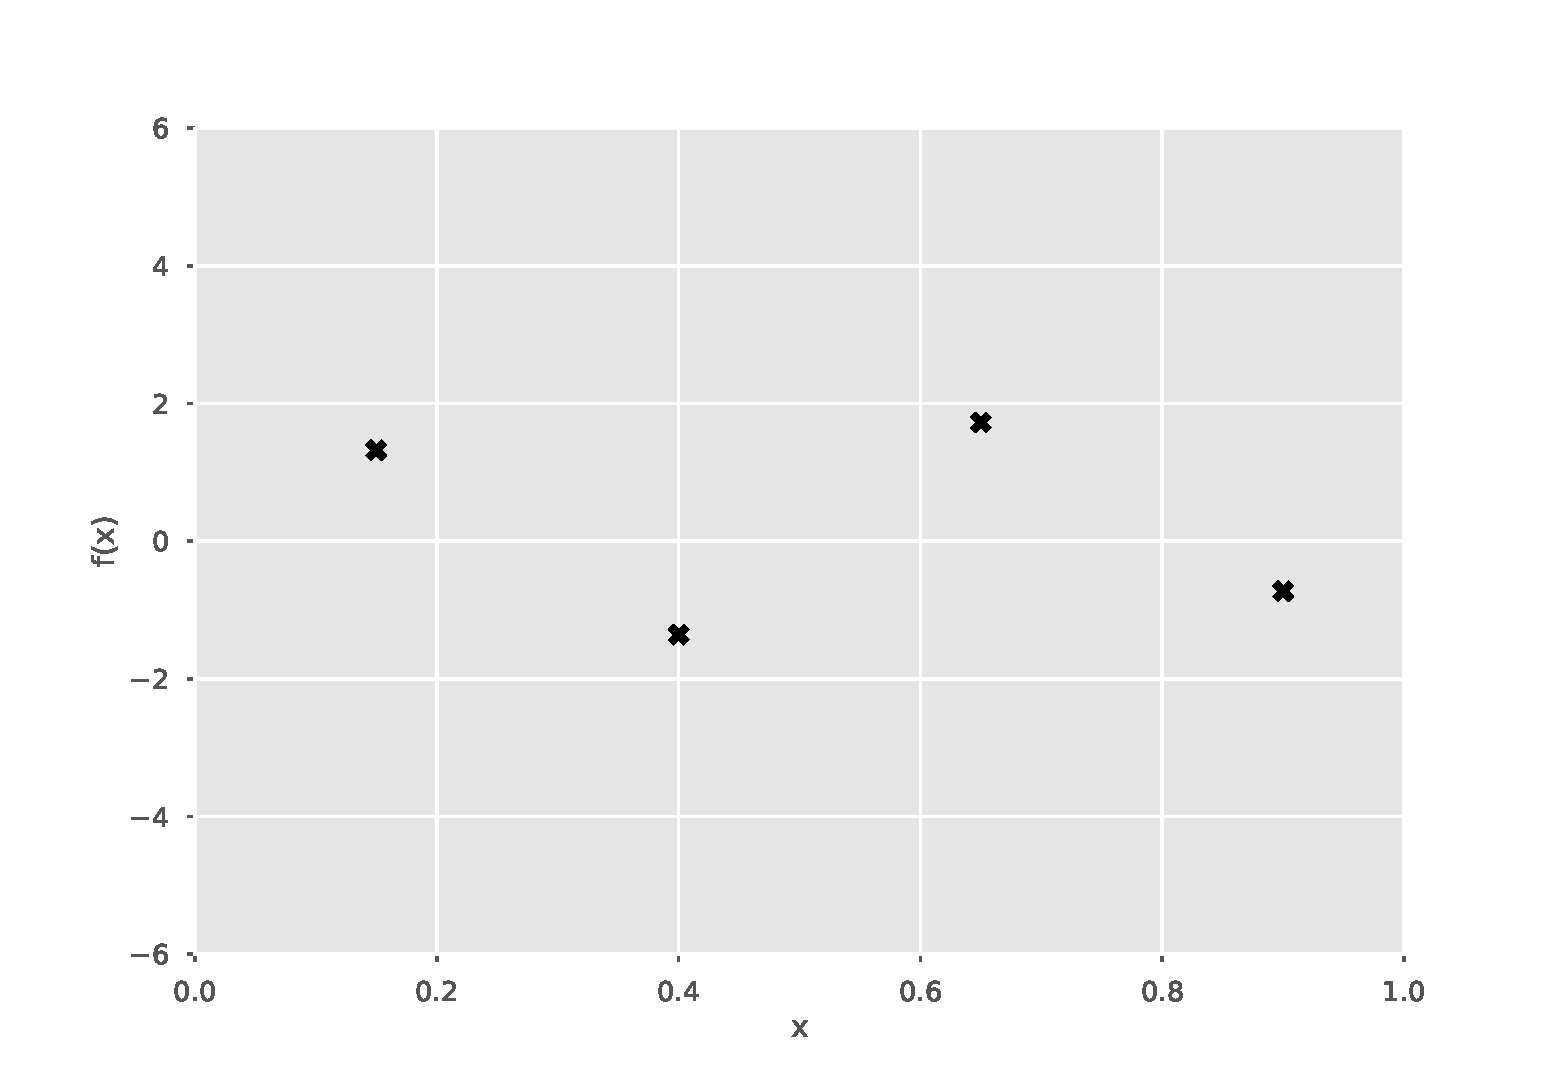
\includegraphics[width=0.8\textwidth, %height=0.38\textwidth]{images/intro_images/plot_datapoints.p%df}
%    \label{fig:my_label}
%\end{figure}
%\begin{center}
%  Where is the minimum of function $f$?  
%\end{center}
%\source{Plots are based on Javier Gonz\'alez's BO lecture %(bo\_intro.py)}



%\end{frame}

%-----------------------------------------------------------------------
%----------------------------------------------------------------------
%\begin{frame}[c]{Problem description}
%\framesubtitle{One possible curve}
%\begin{figure}
%    \centering
%    \includegraphics[width=0.7\textwidth, %height=0.4\textwidth]{images/intro_images/plot_posterior_1_s%ample.pdf}
%    \label{fig:my_label}
%\end{figure}
%\source{Plots are based on Javier Gonz\'alez's BO lecture %(bo\_intro.py)}



%\end{frame}

%-----------------------------------------------------------------------
%----------------------------------------------------------------------
%\begin{frame}[c]{Problem description}
%\framesubtitle{Three possible curves}
%\begin{figure}
%    \centering
%    \includegraphics[width=0.7\textwidth, %height=0.4\textwidth]{images/intro_images/plot_posterior_3_s%ample.pdf}
%    \label{fig:my_label}
%\end{figure}
%\source{Plots are based on Javier Gonz\'alez's BO lecture %(bo\_intro.py)}



%\end{frame}

%-----------------------------------------------------------------------
%----------------------------------------------------------------------
%\begin{frame}[c]{Problem description}
%\framesubtitle{Ten possible curves}
%\begin{figure}
%    \centering
%    \includegraphics[width=0.7\textwidth, %height=0.4\textwidth]{images/intro_images/plot_posterior_10_%sample.pdf}
%    \label{fig:my_label}
%\end{figure}
%\source{Plots are based on Javier Gonz\'alez's BO lecture %(bo\_intro.py)}



%\end{frame}

%-----------------------------------------------------------------------
%----------------------------------------------------------------------
%\begin{frame}[c]{Problem description}
%\framesubtitle{One hundred possible curves}
%\begin{figure}
%    \centering
%    \includegraphics[width=0.7\textwidth, %height=0.4\textwidth]{images/intro_images/plot_posterior_100%_sample.pdf}
%    \label{fig:my_label}
%\end{figure}
%\source{Plots are based on Javier Gonz\'alez's BO lecture %(bo\_intro.py)}



%\end{frame}

%-----------------------------------------------------------------------%----------------------------------------------------------------------
%\begin{frame}[c]{Problem description}
%\framesubtitle{One thousand possible curves}
%\begin{figure}
%    \centering
%    \includegraphics[width=0.7\textwidth, %height=0.4\textwidth]{images/intro_images/plot_posterior_100%0_sample.pdf}
%    \label{fig:my_label}
%\end{figure}
%\source{Plots are based on Javier Gonz\'alez's BO lecture (bo\_intro.py)}



%\end{frame}

%-----------------------------------------------------------------------
%----------------------------------------------------------------------
%\begin{frame}[c]{Problem description}
%\framesubtitle{Infinitely many curves}
%\begin{figure}
%    \centering
%    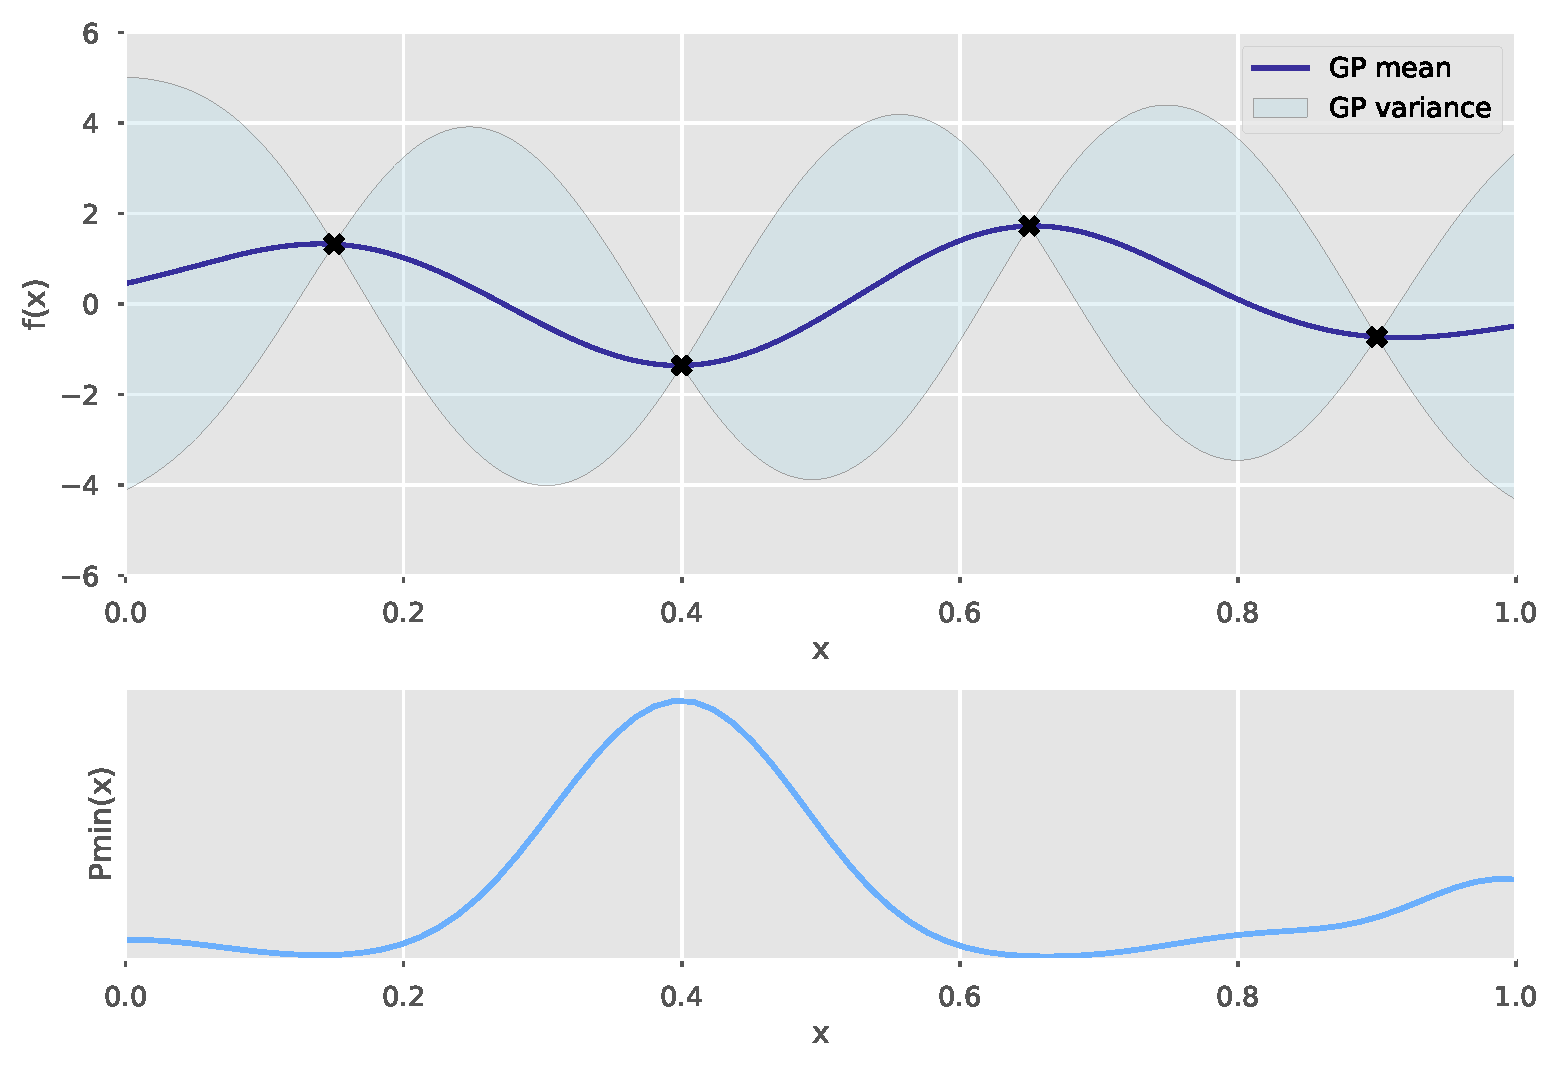
\includegraphics[width=0.7\textwidth, %height=0.4\textwidth]{images/intro_images/plot_posterior.pdf%}
%    \label{fig:my_label}
%\end{figure}
%\source{Plots are based on Javier Gonz\'alez's BO lecture (bo\_intro.py)}


%\end{frame}
%----------------------------------------------------------------------
\myframetop{Bayesian Optimization of a blackbox function in a nutshell}{

\bigskip
\bigskip
\bigskip

    \onslide<1->
    \begin{figure}
        \vspace{-1em}
        \centering
        \only<1>{
            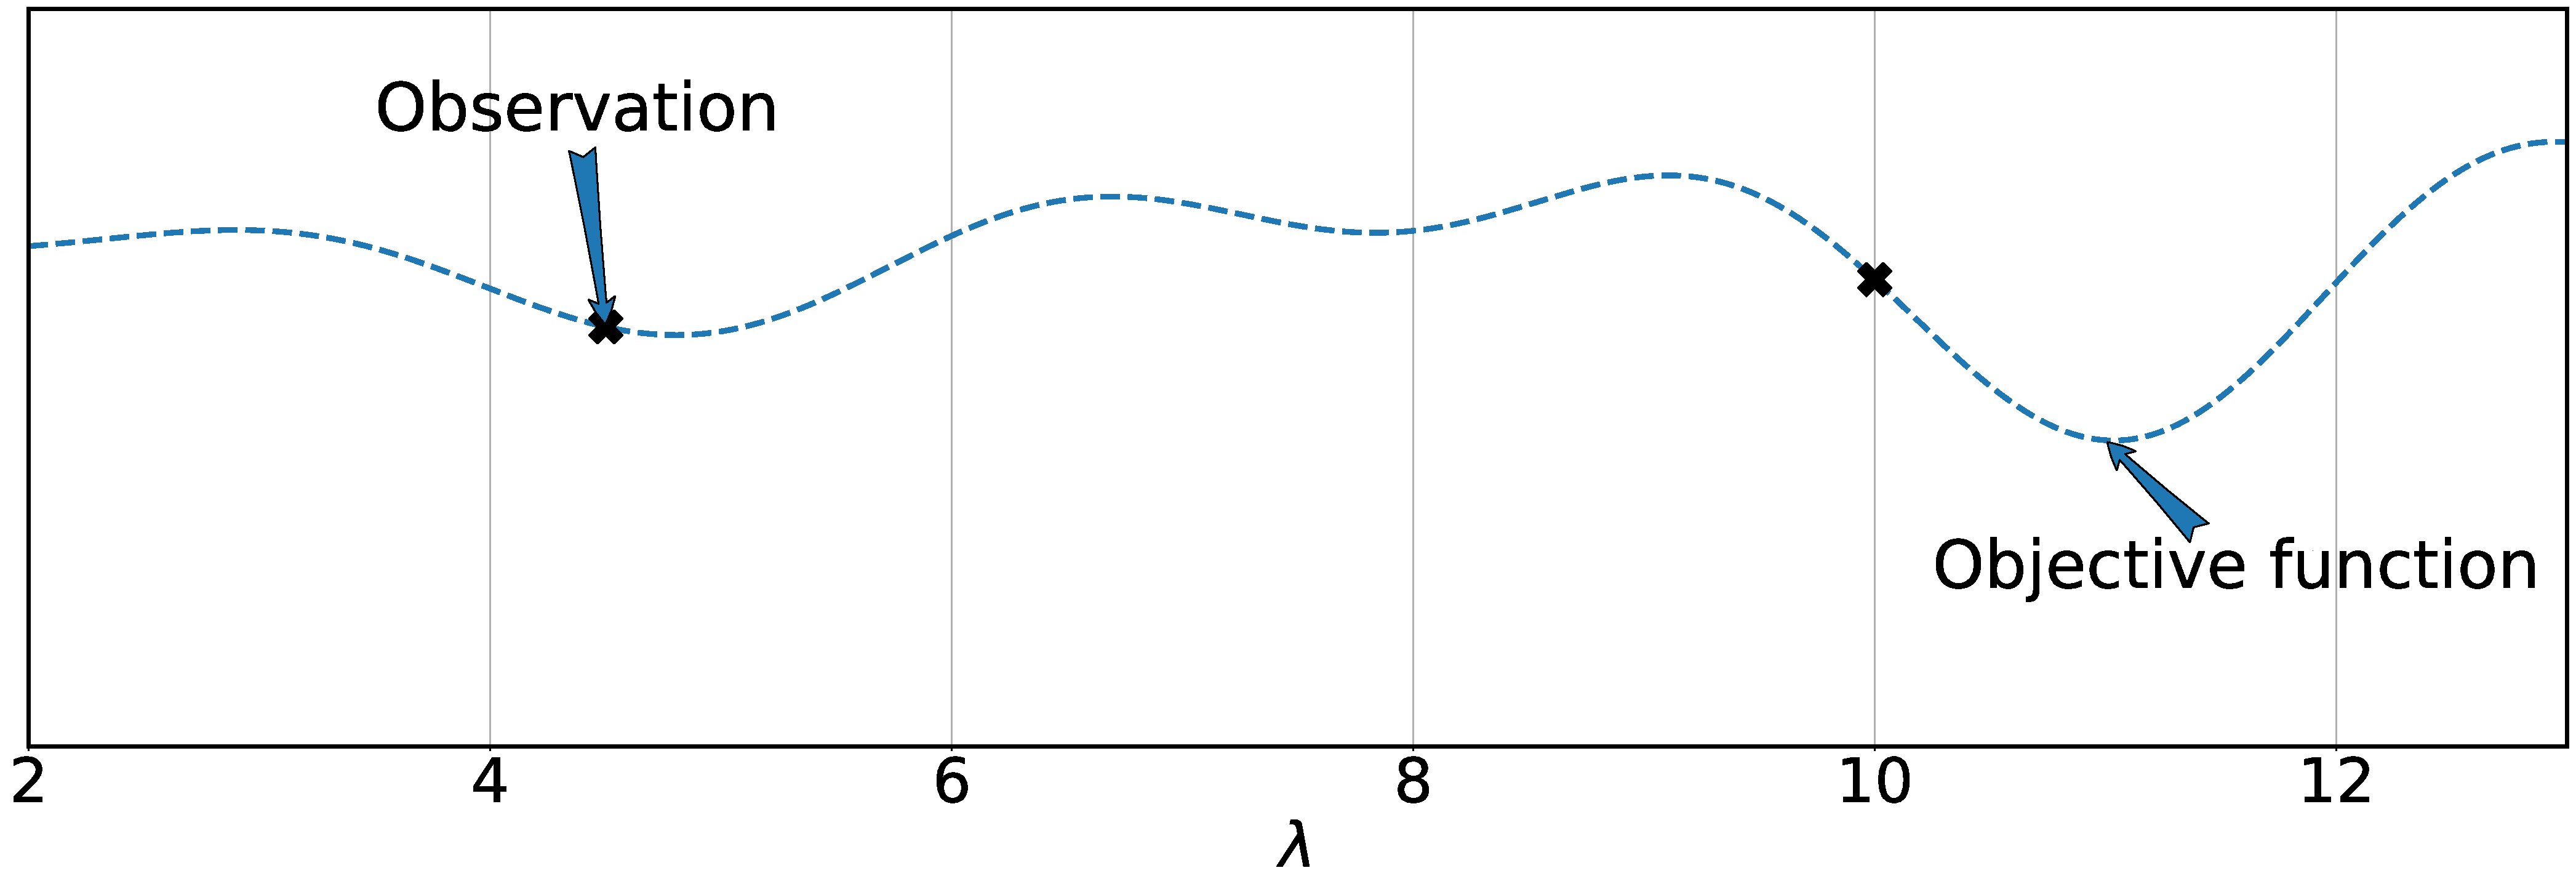
\includegraphics[width=0.95\textwidth]{images/intro_images/IntroPlots_Obs.pdf}
        }\only<2>{
            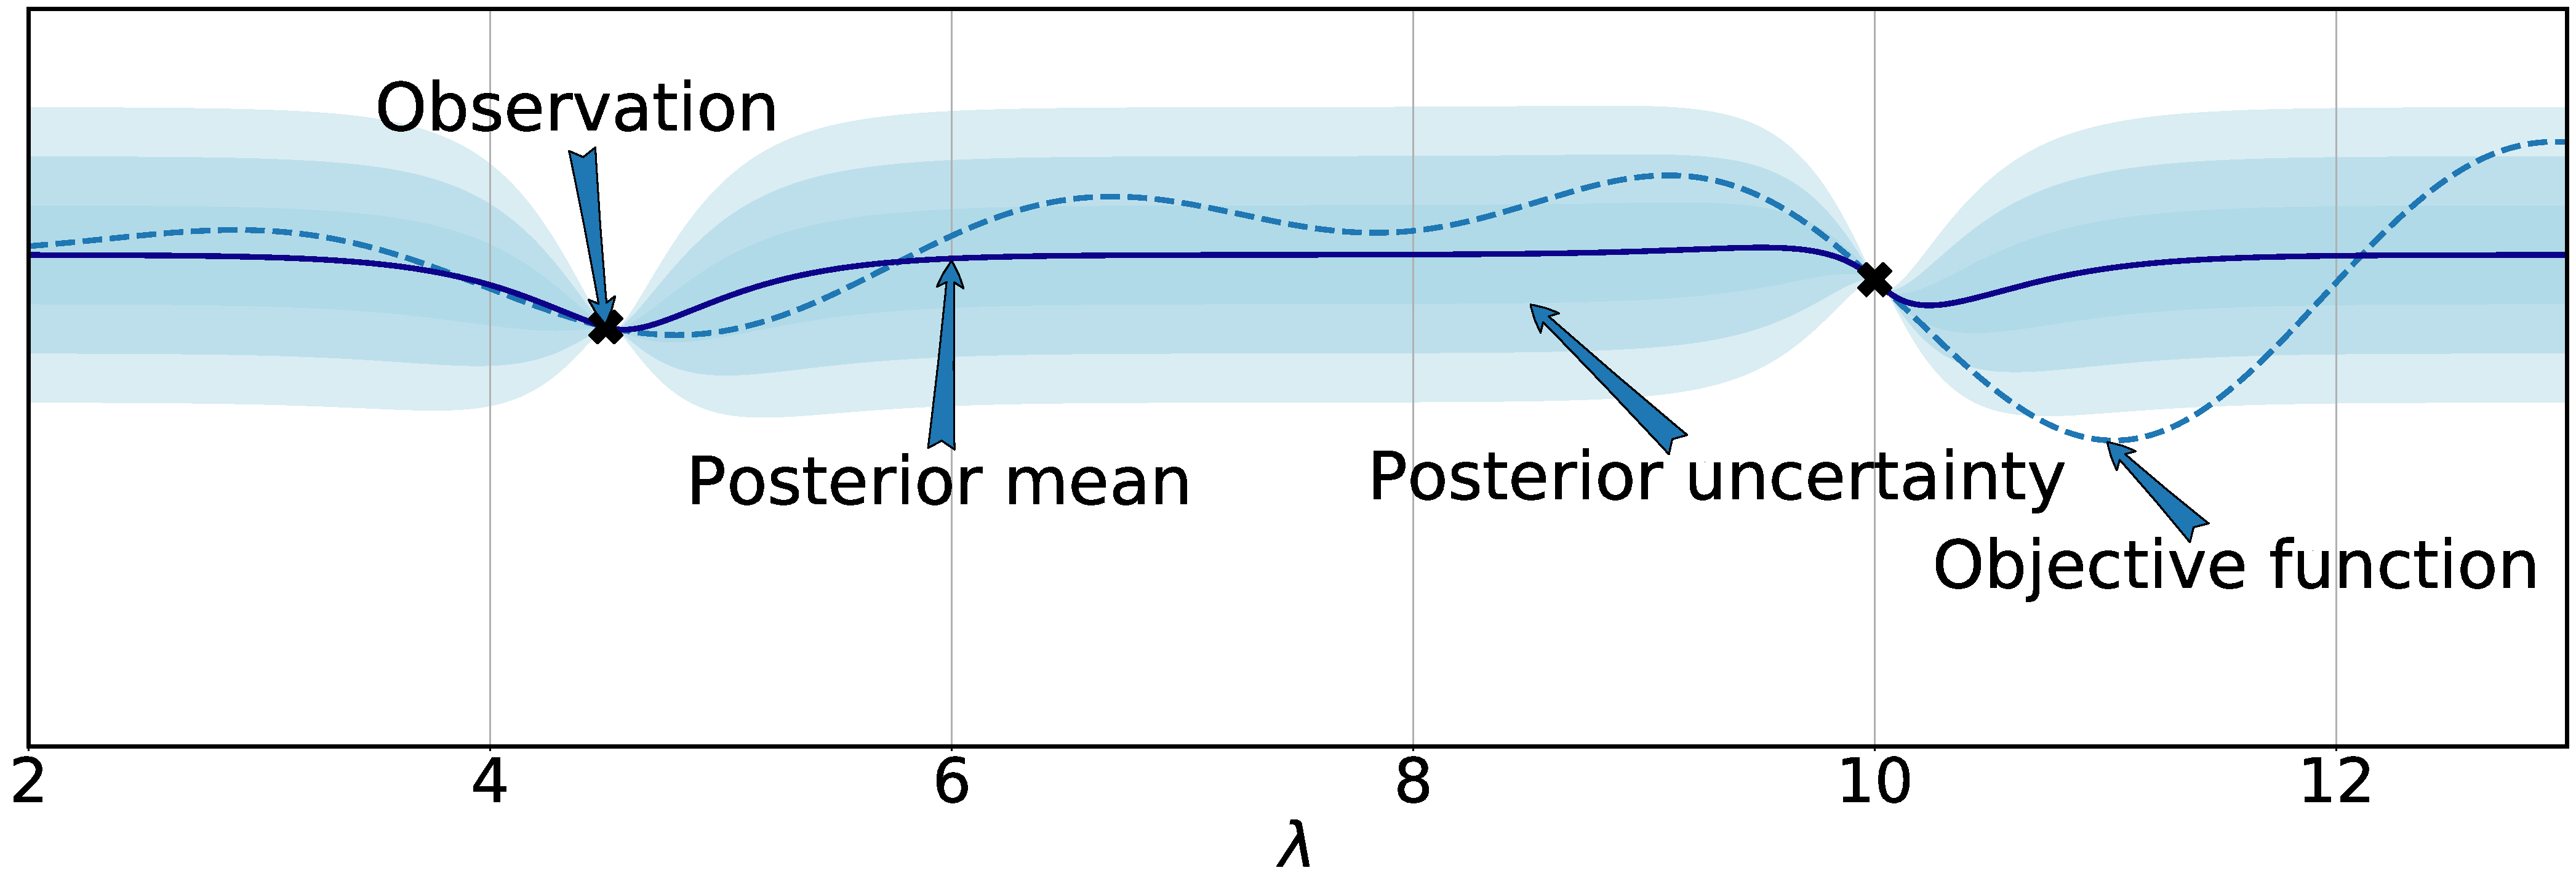
\includegraphics[width=0.95\textwidth]{images/intro_images/IntroPlots_GP.pdf}
        }\only<3>{
            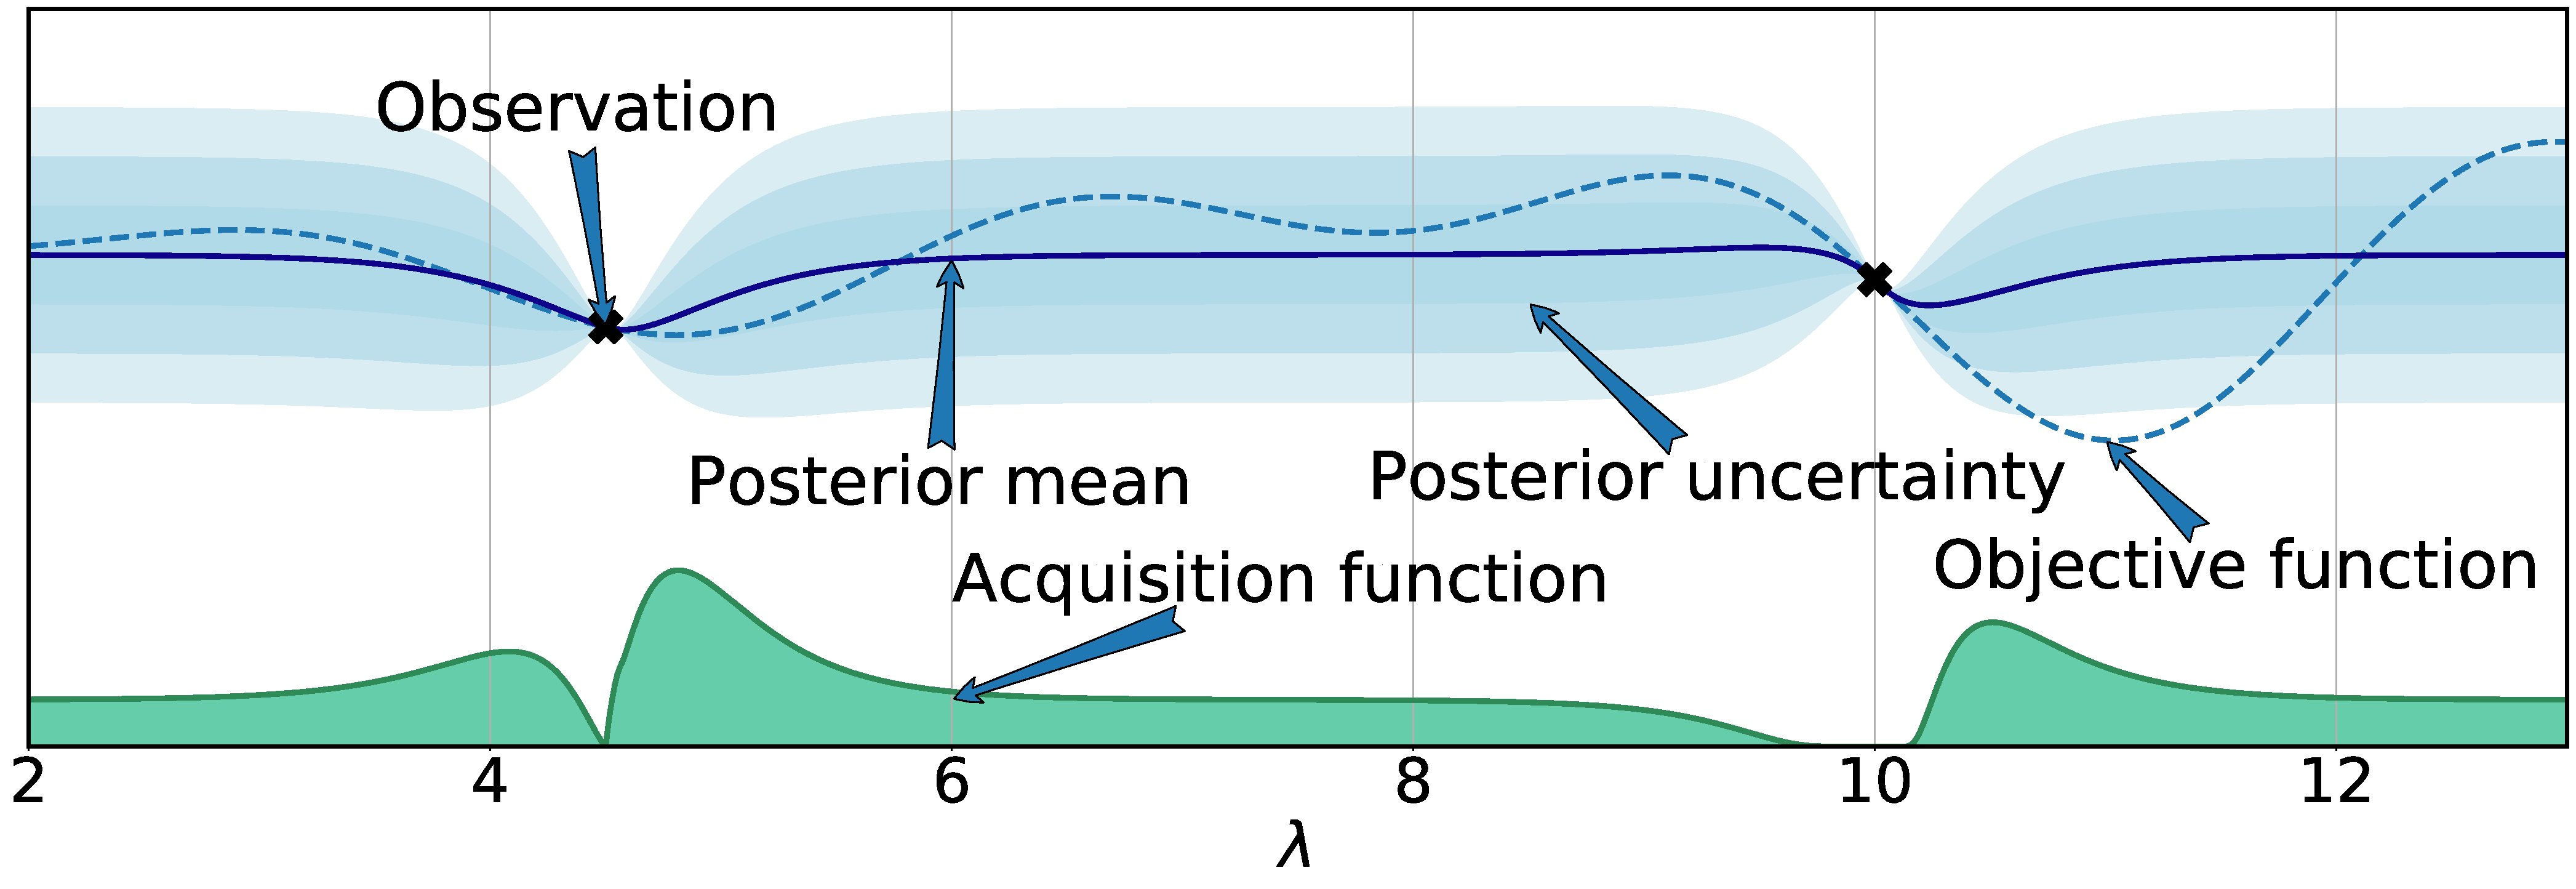
\includegraphics[width=0.95\textwidth]{images/intro_images/IntroPlots_Acqui.pdf}
        }\only<4->{
            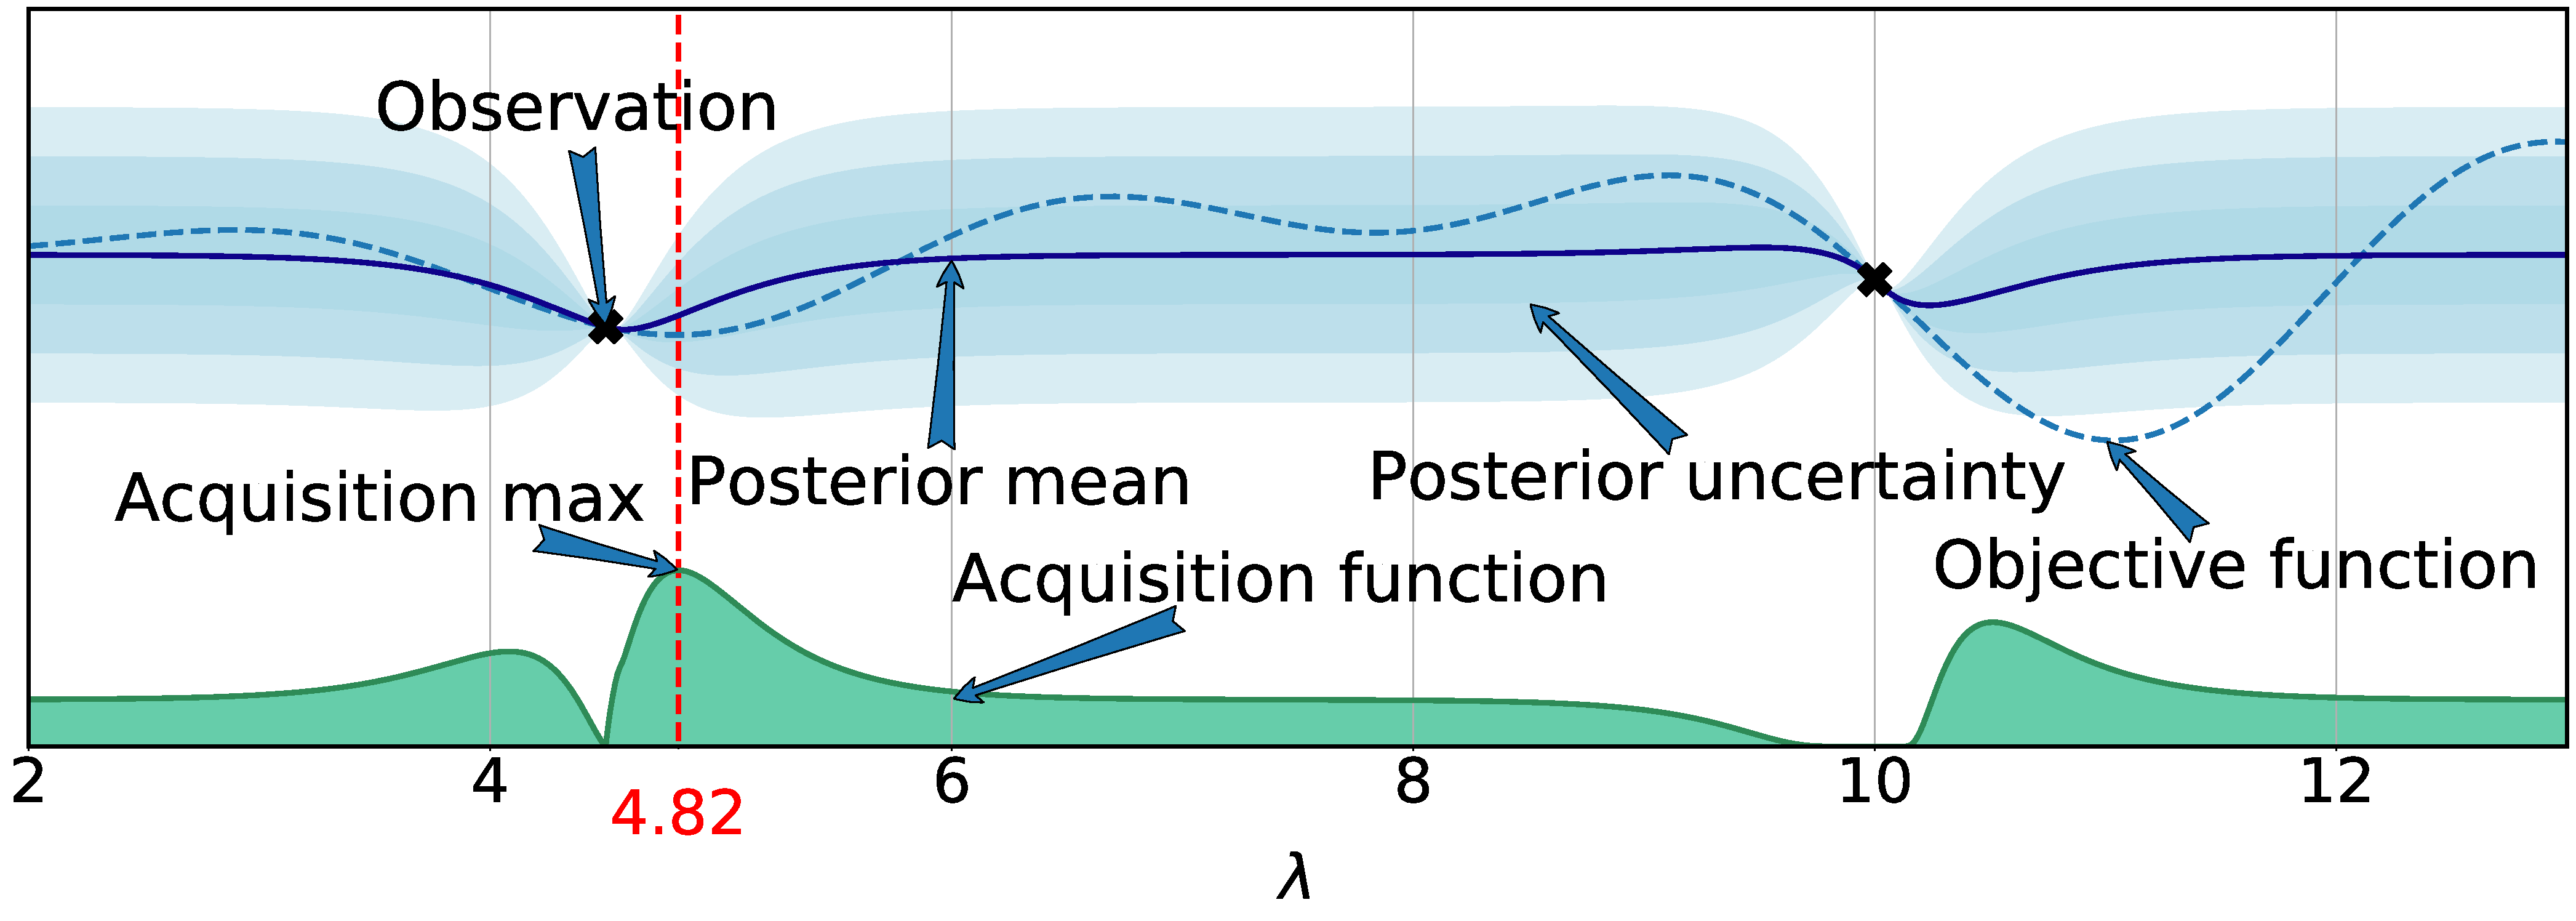
\includegraphics[width=0.95\textwidth]{images/intro_images/IntroPlots_Complete.pdf}
        }
    \end{figure}
    
% \vspace*{-0.5cm}\notefh{Can you please increase the plotted values of the acquisition function, so that it is more clearly visible? Also on the next slide. You could, e.g., normalize it to have a certain maximum (a bit larger than that of the third plot on the next slide). Also, on the next slide, can you please plot the new observation red, not green?}
}

%----------------------------------------------------------------------
\begin{frame}[c]{Bayesian Optimization of a blackbox function in a nutshell}

\begin{columns}[T]
\column{0.45\textwidth}
General approach
\begin{itemize}
    \item Fit a \alert{probabilistic model} to the collected function samples $\langle{}\conf, \cost(\conf)\rangle{}$
    \item Use the model to guide optimization, trading off \alert{exploration \vs{} exploitation}
%    \item Acquisition function for exploration-exploitation tradeoff
%    \item Optimize on acquisition function\\ to get next $x$ $\conf$ ($x$)
\end{itemize}

\bigskip

\onslide<4->{
    \alert{Popular approach in the statistics literature} since
    \href{http://link.springer.com/chapter/10.1007\%2F3-540-07165-2_55}{\footnotesize\color{black!70} Mockus et al. [1978]}
    \begin{itemize}
        \item Efficient in \#function evaluations
        \item Works when objective is \alert{nonconvex, noisy, has unknown derivatives, etc.}
        \item Recent \alert{convergence} results\\ \lit{\href{https://arxiv.org/abs/0912.3995}{Srinivas et al. 2009}; \href{http://www.jmlr.org/papers/v12/bull11a.html}{Bull et al. 2011}; \href{https://www.cs.ubc.ca/~nando/papers/BayesBandits.pdf}{de Freitas et al. 2012}; \href{http://papers.nips.cc/paper/5715-bayesian-optimization-with-exponential-convergence}{Kawaguchi et al. 2015}}
    %    \item Popular \alert{Bayesian optimization workshop} at NIPS (the premiere machine learning conference)
    \end{itemize}
}

\column{0.55\textwidth}
\onslide<1->
\begin{figure}
    \vspace{-1em}
    \centering
    \onslide<1->{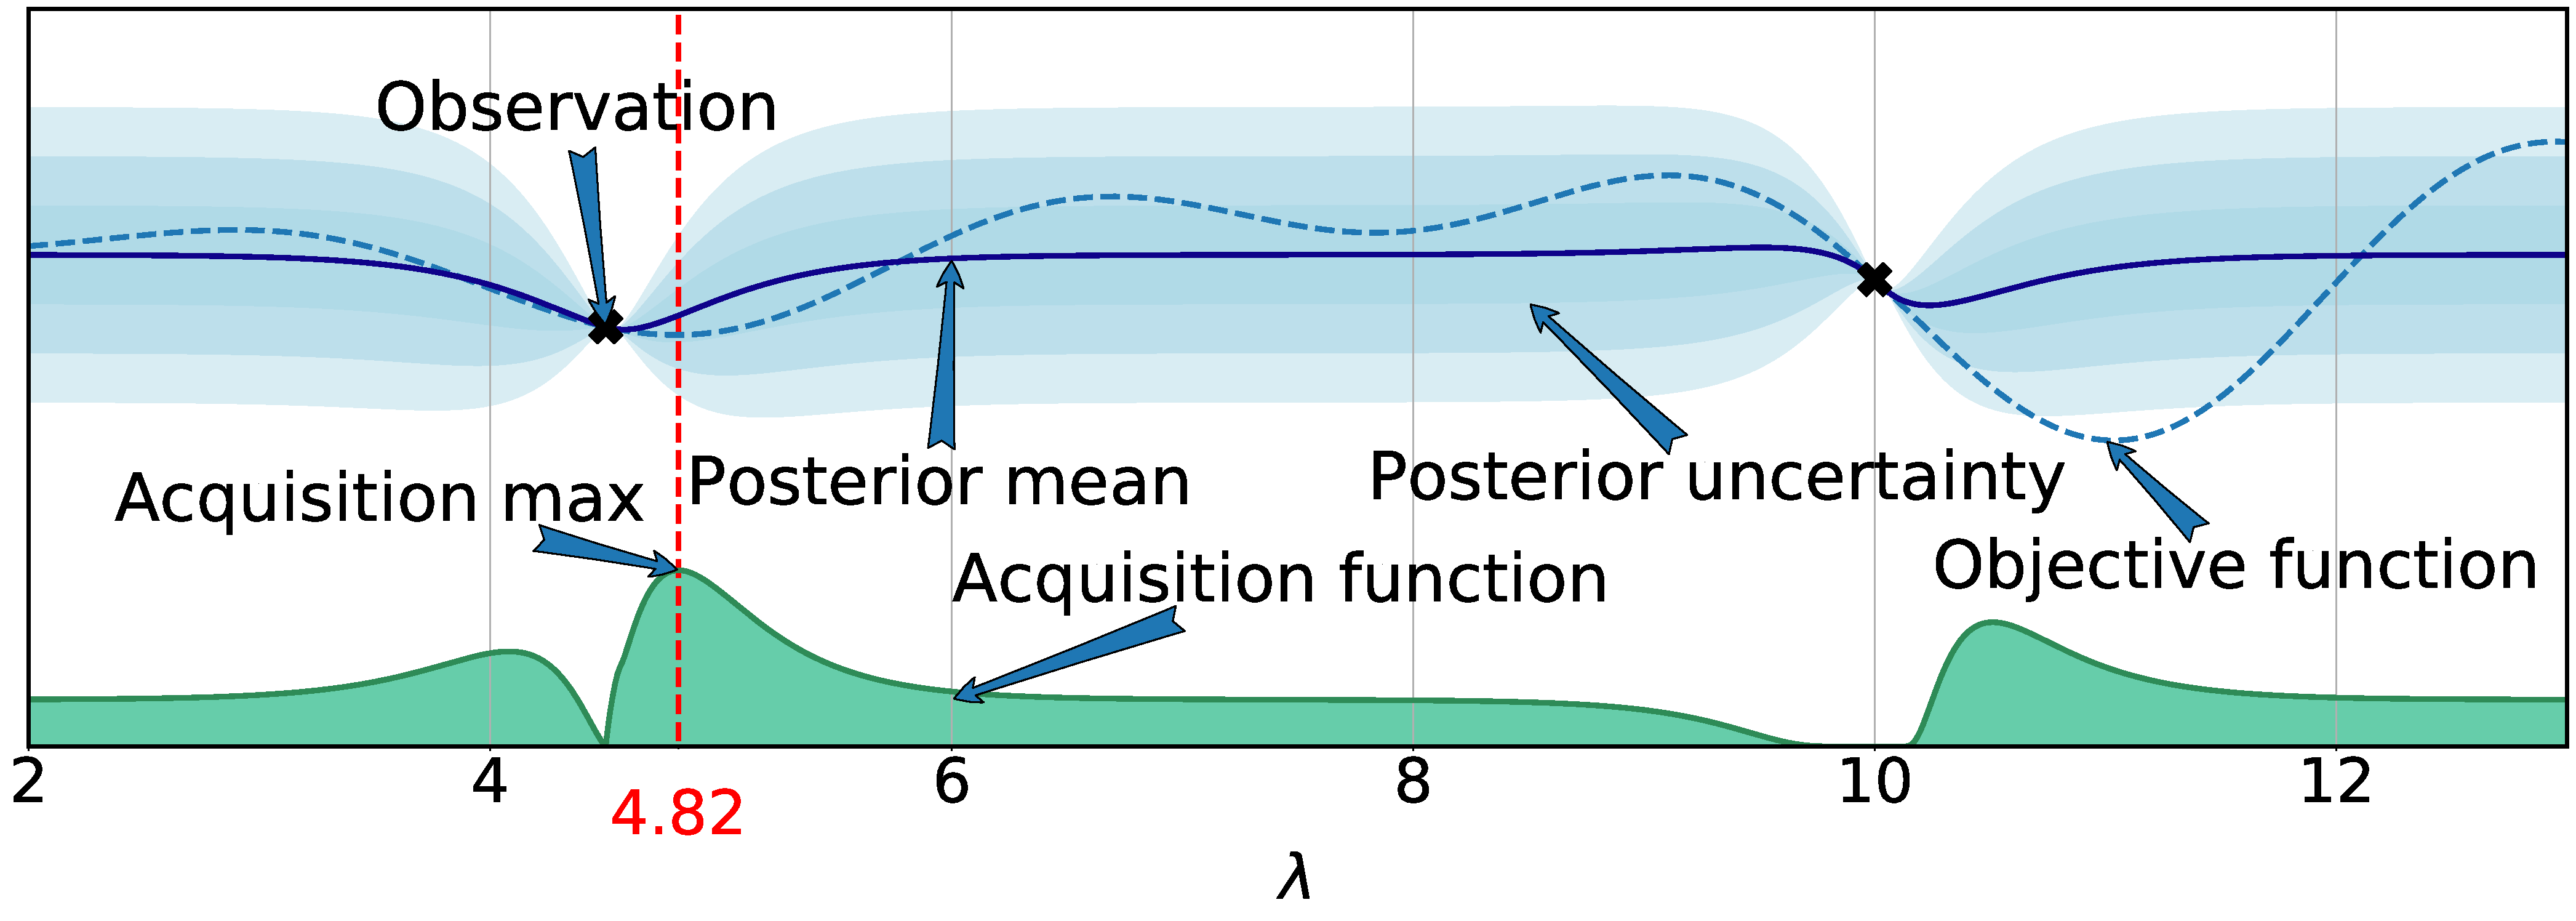
\includegraphics[width=0.8\textwidth]{images/intro_images/IntroPlots_Iter2.pdf}}
    \onslide<2->{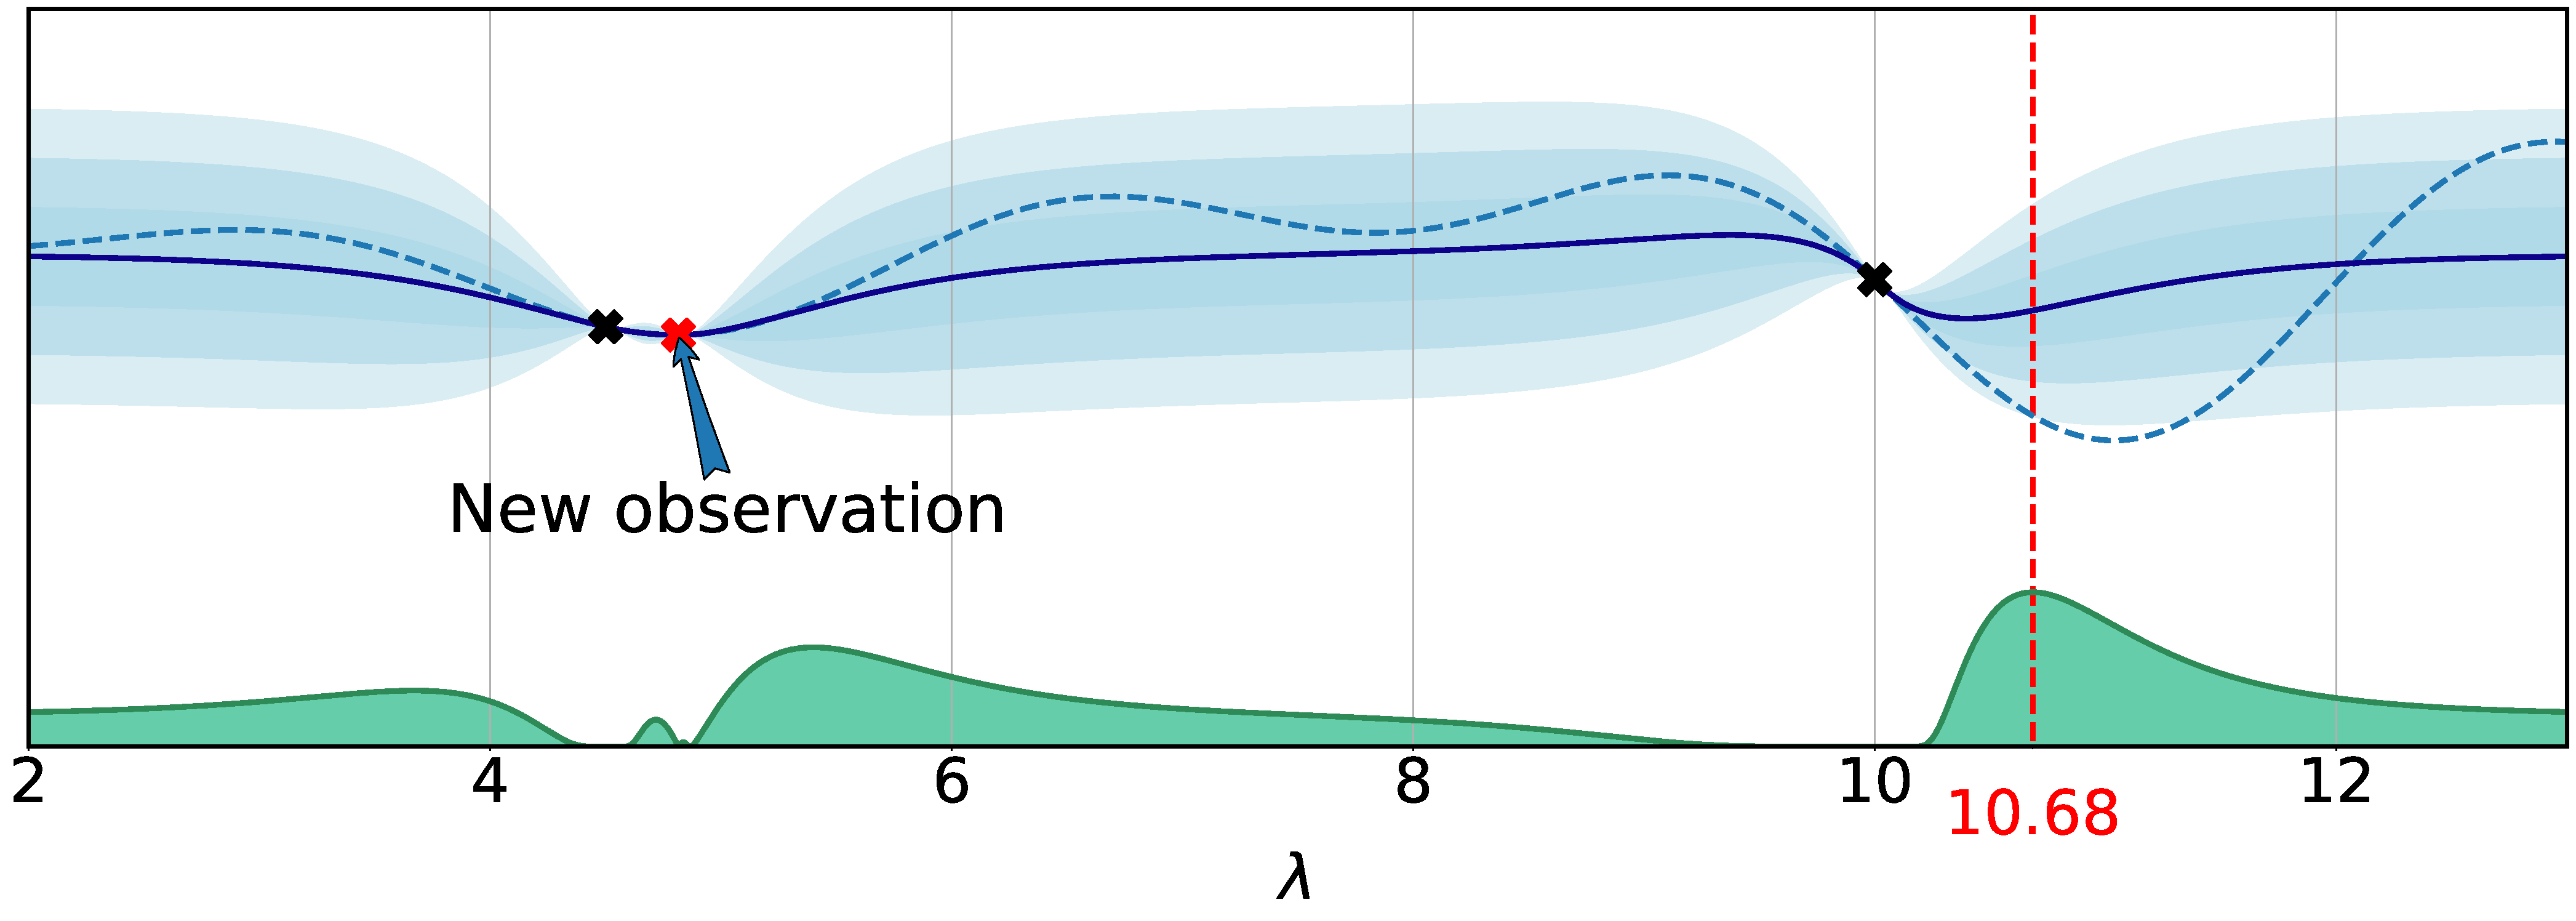
\includegraphics[width=0.8\textwidth]{images/intro_images/IntroPlots_Iter3.pdf}}
    \onslide<3->{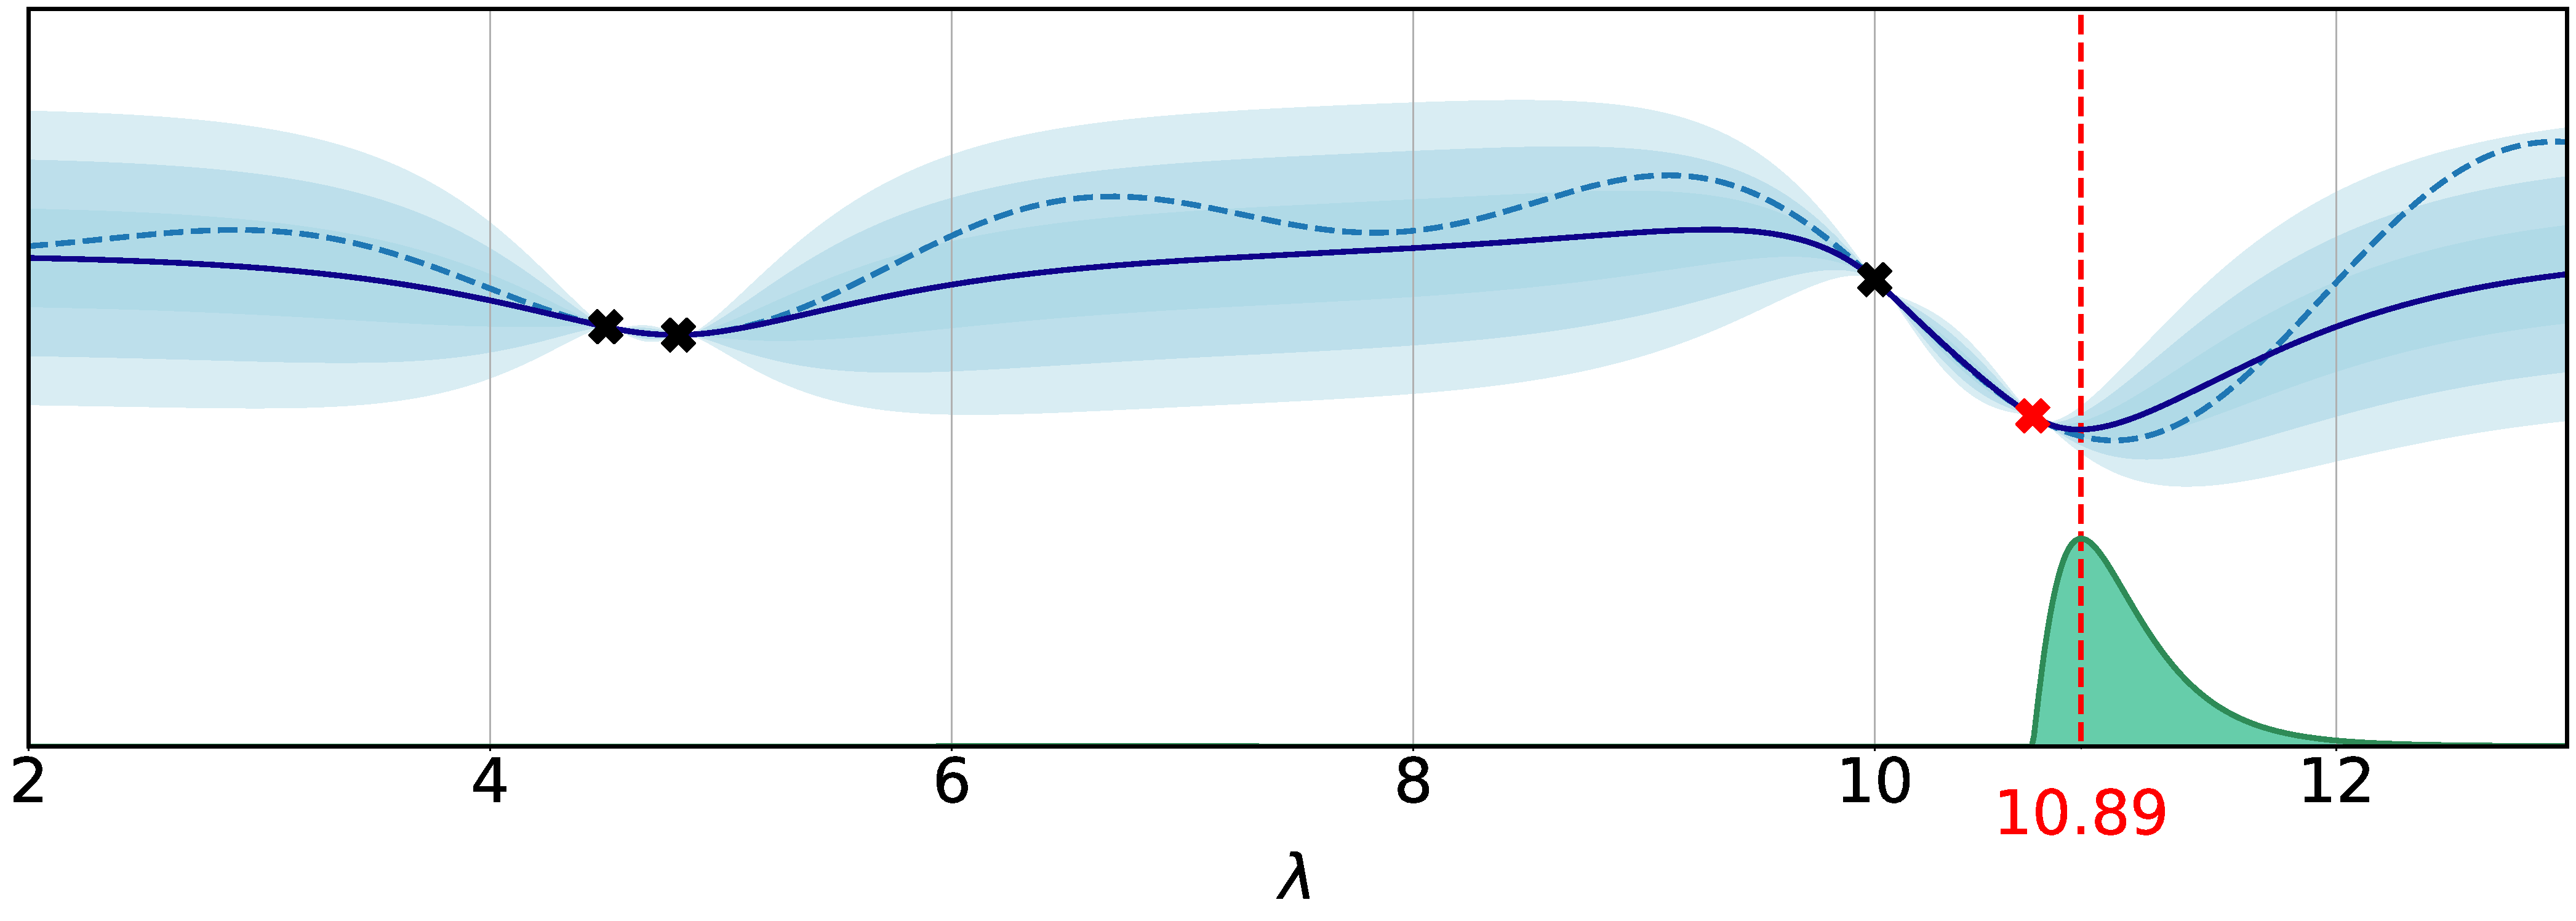
\includegraphics[width=0.8\textwidth]{images/intro_images/IntroPlots_Iter4.pdf}}
    %\only<4>{\includegraphics[width=\textwidth]{images/intro_images/plot_2.pdf}}
    %\only<5>{\includegraphics[width=\textwidth]{images/intro_images/plot_3.pdf}}
    %\only<6>{\includegraphics[width=\textwidth]{images/intro_images/plot_4.pdf}}
    %\only<7>{\includegraphics[width=\textwidth]{images/intro_images/plot_5.pdf}}
    %\only<8>{\includegraphics[width=\textwidth]{images/intro_images/plot_6.pdf}}
    %\only<9->{\includegraphics[width=\textwidth]{images/intro_images/plot_7.pdf}}
\end{figure}
\end{columns}

\end{frame}
%-----------------------------------------------------------------------
%\myframe{Bayesian Optimization in a Nutshell}{
%  
%\vspace*{-0.5cm}
%\begin{columns}[T]
%
%\column{0.6\textwidth}
%
%\myblock{General approach}{
%	\myit{
%	  \item Fit a probabilistic model to the collected function samples
%	  $\langle{}\conf, \cost(\conf)\rangle{}$
%	  \item Use the model to guide optimization, trading off
%	  exploration \vs{} exploitation
%	%  \item Acquisition function for exploration-exploitation tradeoff
%	%  \item Optimize on acquisition function\\ to get next $x$
%	  %$\conf$ ($x$)
%	}
%}
%
%\smallskip
%\onslide<5->{
%	\myblock{Popular approach in the statistics literature since \litw{\href{http://link.springer.com/chapter/10.1007\%2F3-540-07165-2_55}{Mockus,
%	1978}}}{ \myit{
%		  	\item Efficient in \# function evaluations 
%		  	\item Works when objective is nonconvex, noisy, has unknown derivatives, etc
%			\pause
%			\item Recent convergence results\\ \lit{Srinivas et al, 2010; Bull 2011;
%			de Freitas et al, 2012; Kawaguchi et al, 2015}
%			%TODO: sorry, I don't know these papers
%		%	\item Popular \alert{Bayesian optimization workshop} at NIPS (the premiere machine learning conference)
%		}
%	}
%}
%%\begin{enumerate}
%%  \item Fit an empirical performance model (EPM) 
%%  \item Acquisition function for exploration-exploitation tradeoff
%%  \item Optimize on acquisition function\\ to get next $\conf$ ($x$)
%%\end{enumerate}
%
%\column{0.4\textwidth}
%\vspace*{0.5cm}
%\onslide<2->{
%	%\includegraphics[width=1\textwidth]{../images/bo.png}
%	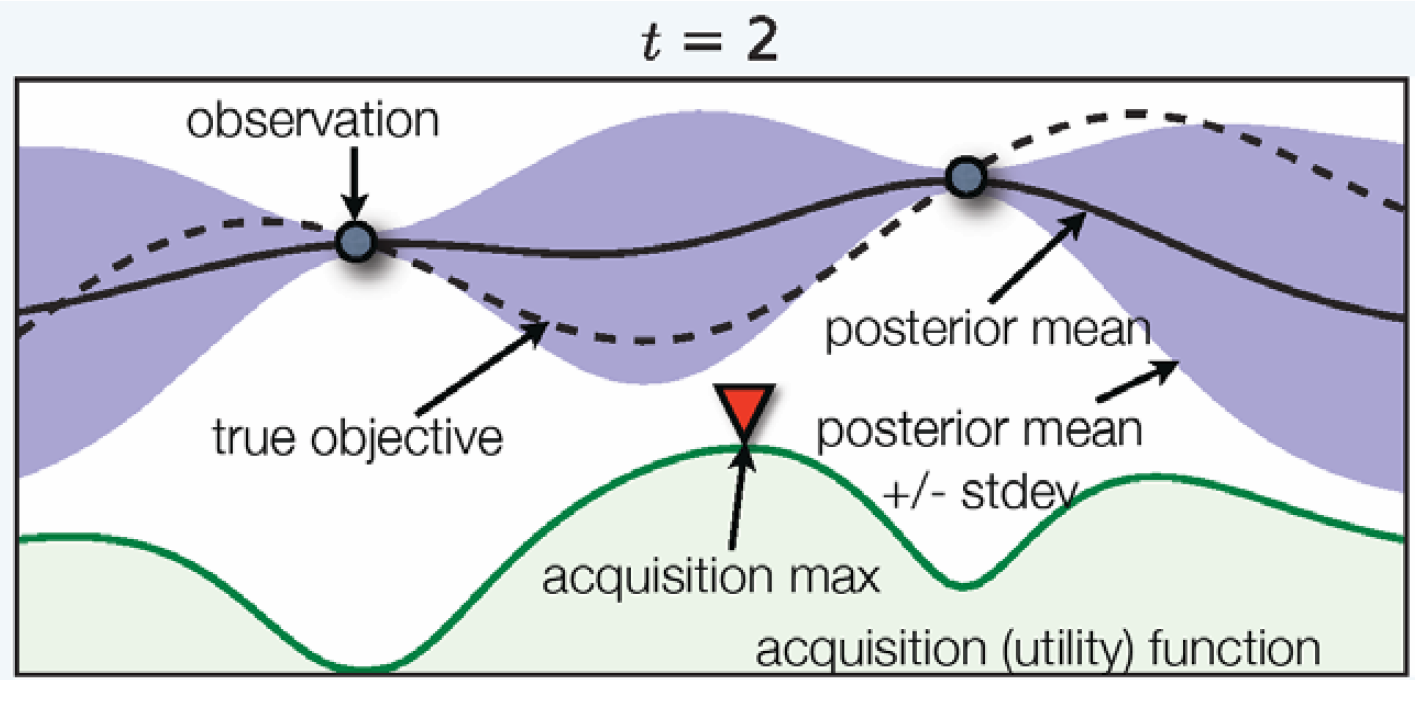
\includegraphics[width=0.9\textwidth]{plots_and_scripts/plots/bo_pic1.png}\\
%	\pause
%	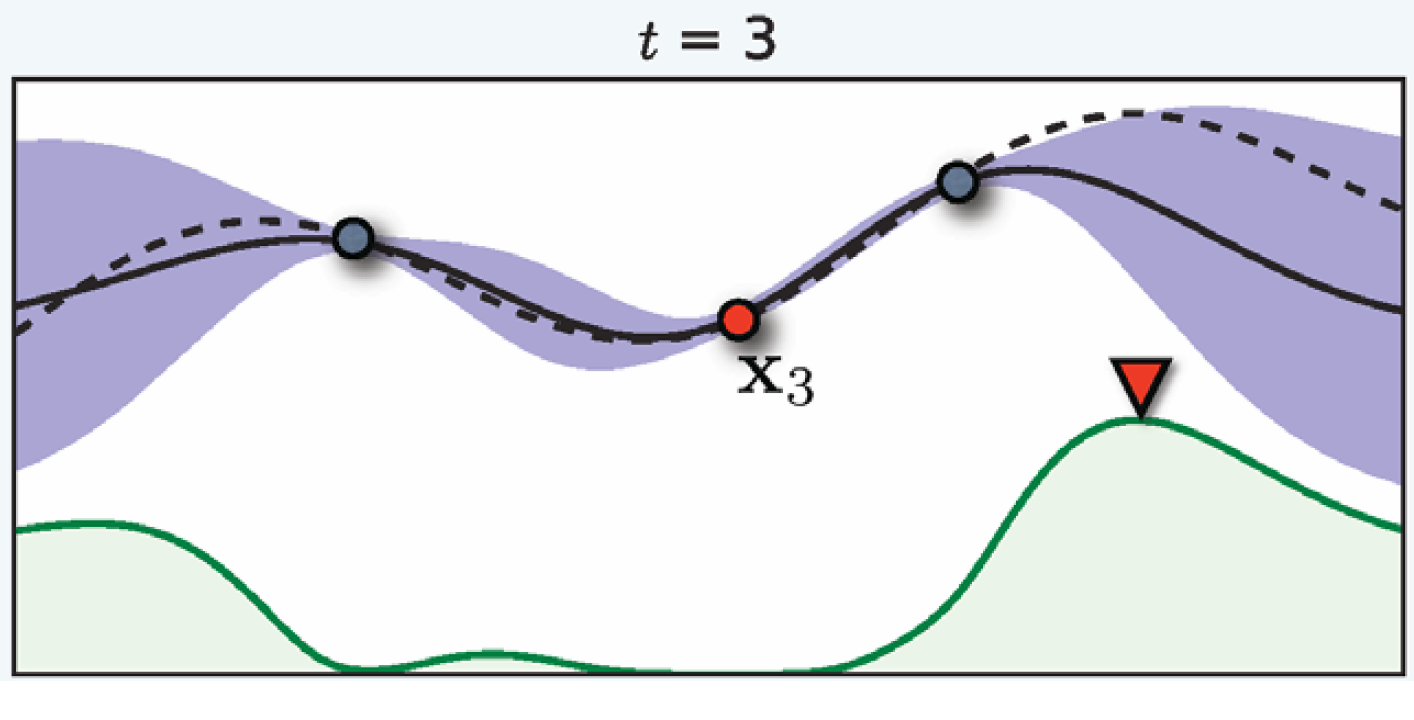
\includegraphics[width=0.9\textwidth]{plots_and_scripts/plots//bo_pic2.png}\\
%	\pause
%	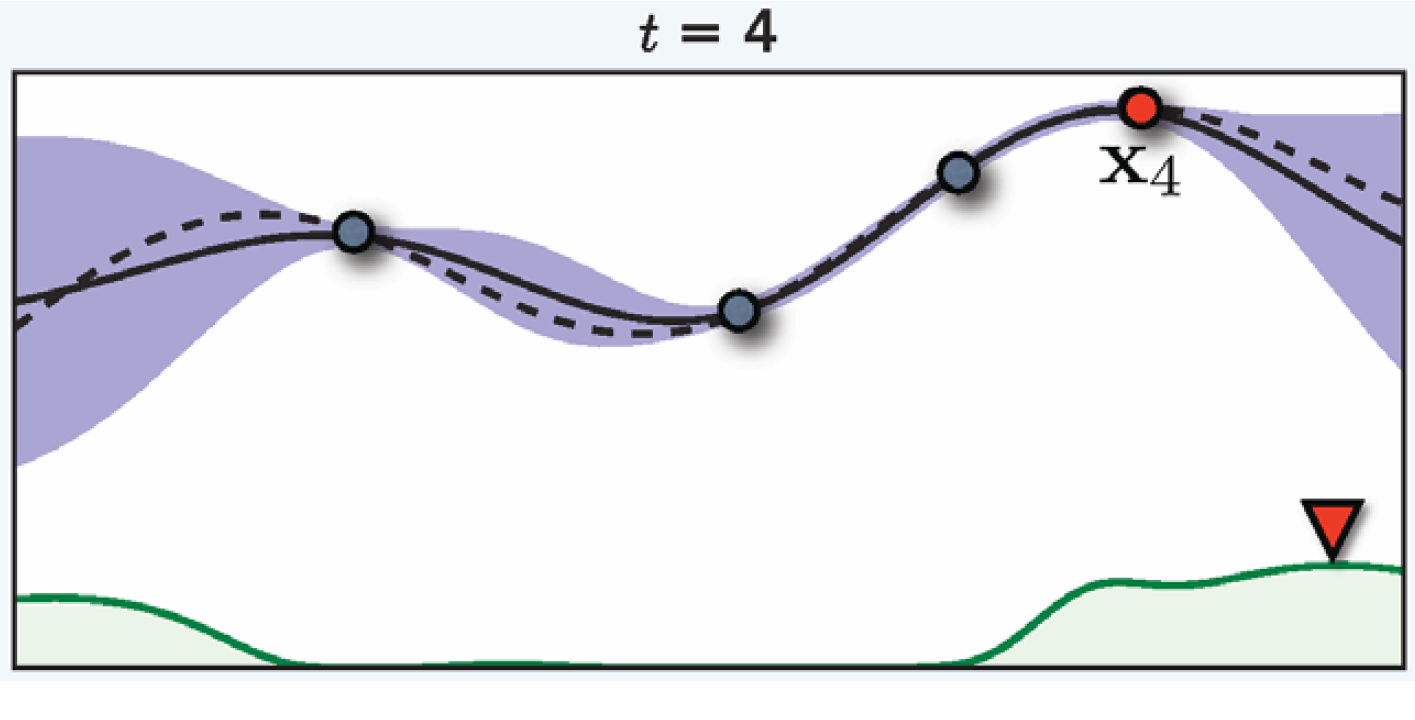
\includegraphics[width=0.9\textwidth]{plots_and_scripts/plots//bo_pic3.png}\\
%	\footnotesize{Image source: \lit{\href{https://arxiv.org/abs/1012.2599}{Brochu et al, 2010}}}
%}
%\end{columns}
%}
%----------------------------------------------------------------------
%5\begin{frame}[c]{Bayesian Optimization: Visualization of Many Steps}
%\begin{figure}
%    \centering
%    \only<1>{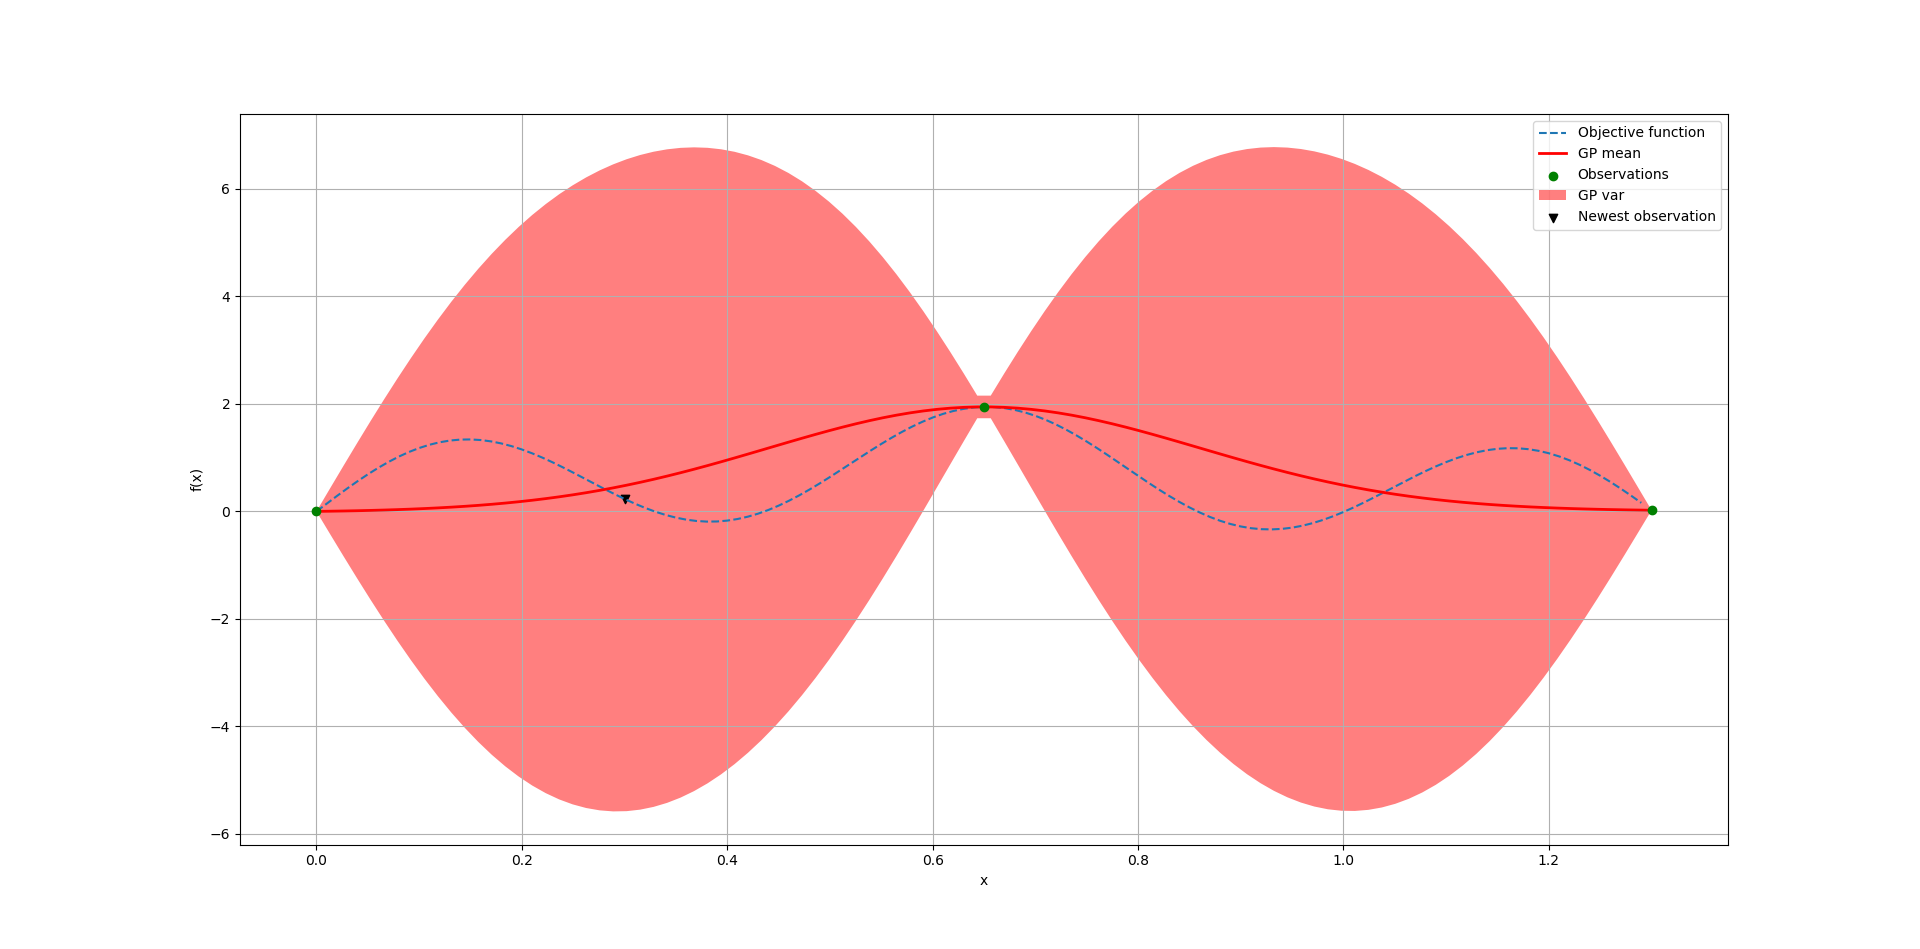
\includegraphics[width=\linewidth]{images/intro_images/BOLoop_1.png}}
%    \only<2>{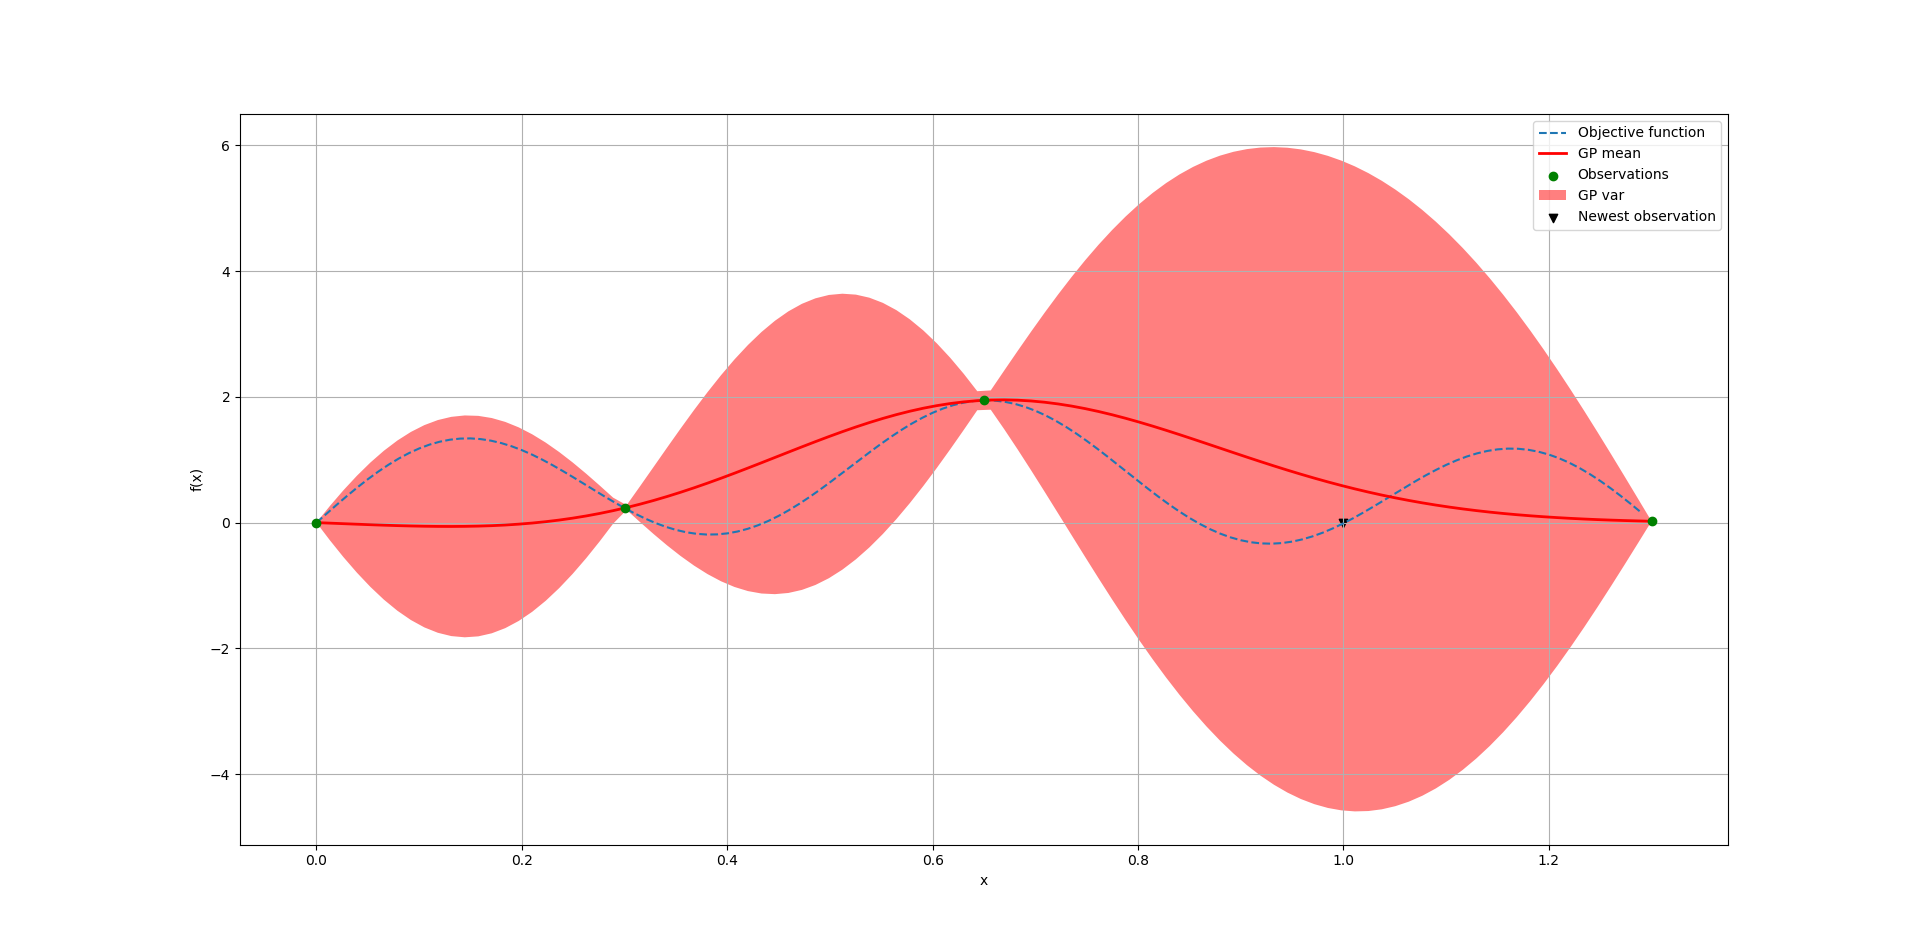
\includegraphics[width=\linewidth]{images/intro_images/BOLoop_2.png}}
%    \only<3>{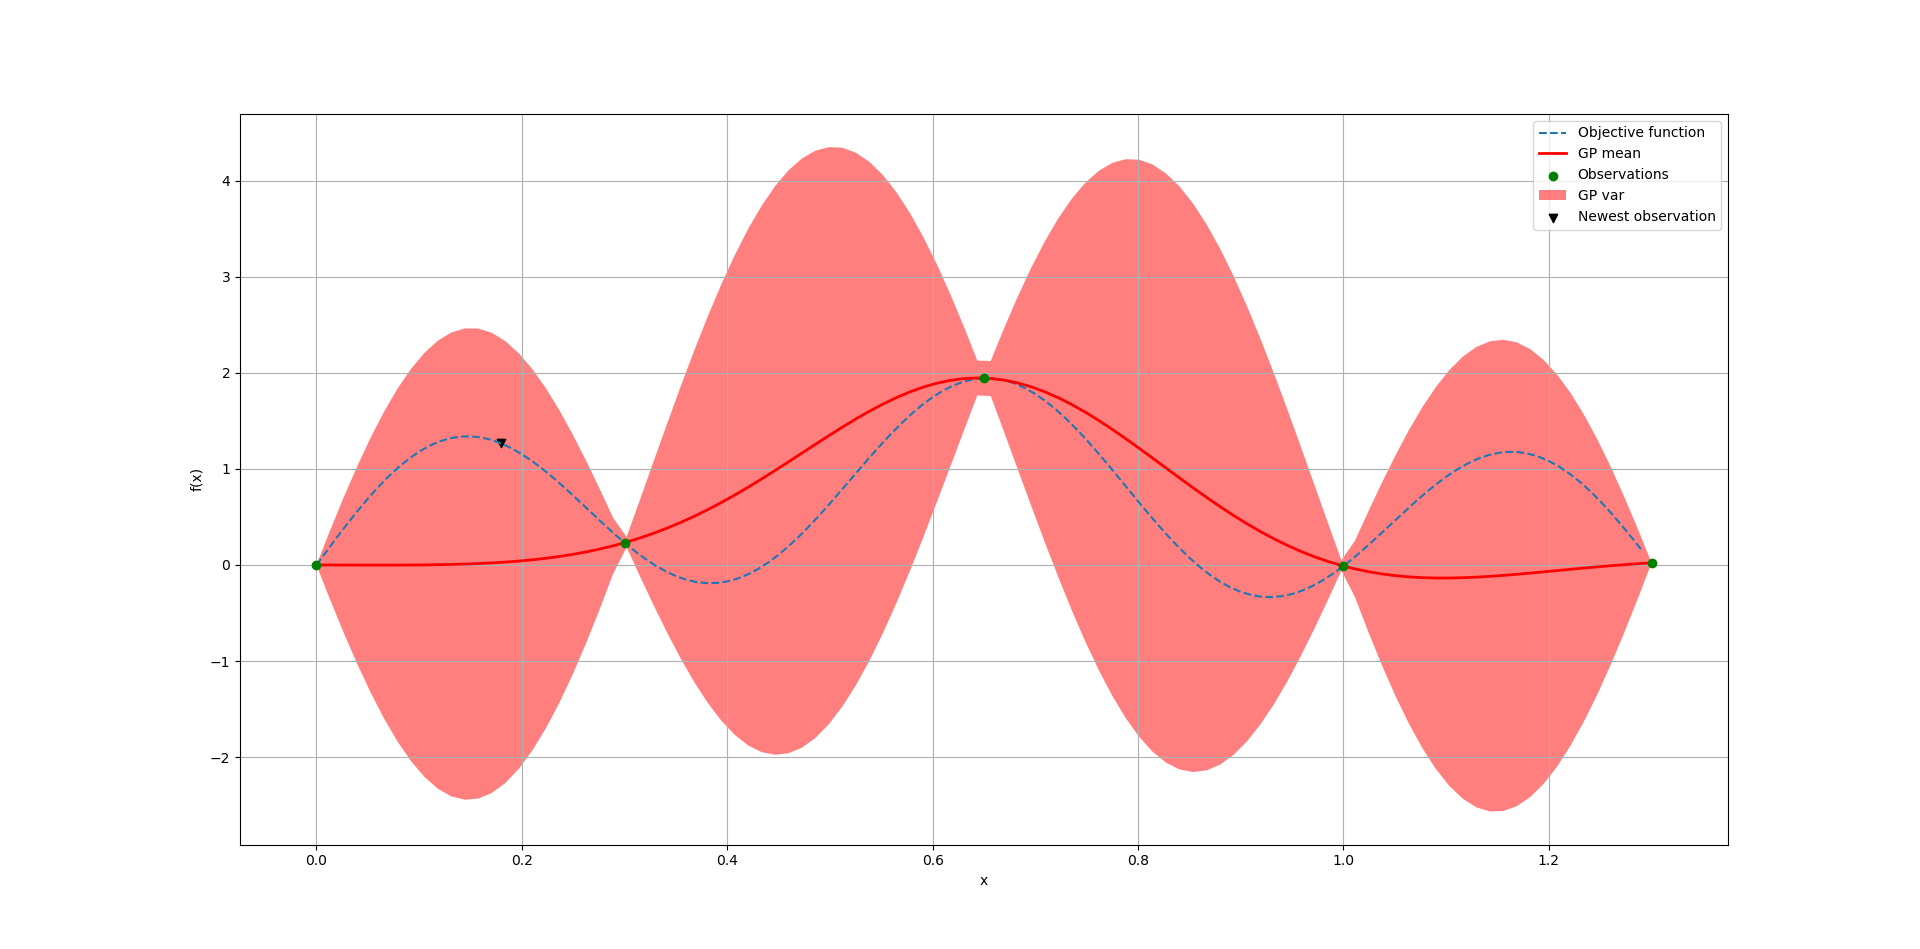
\includegraphics[width=\linewidth]{images/intro_images/BOLoop_3.png}}
%    \only<4>{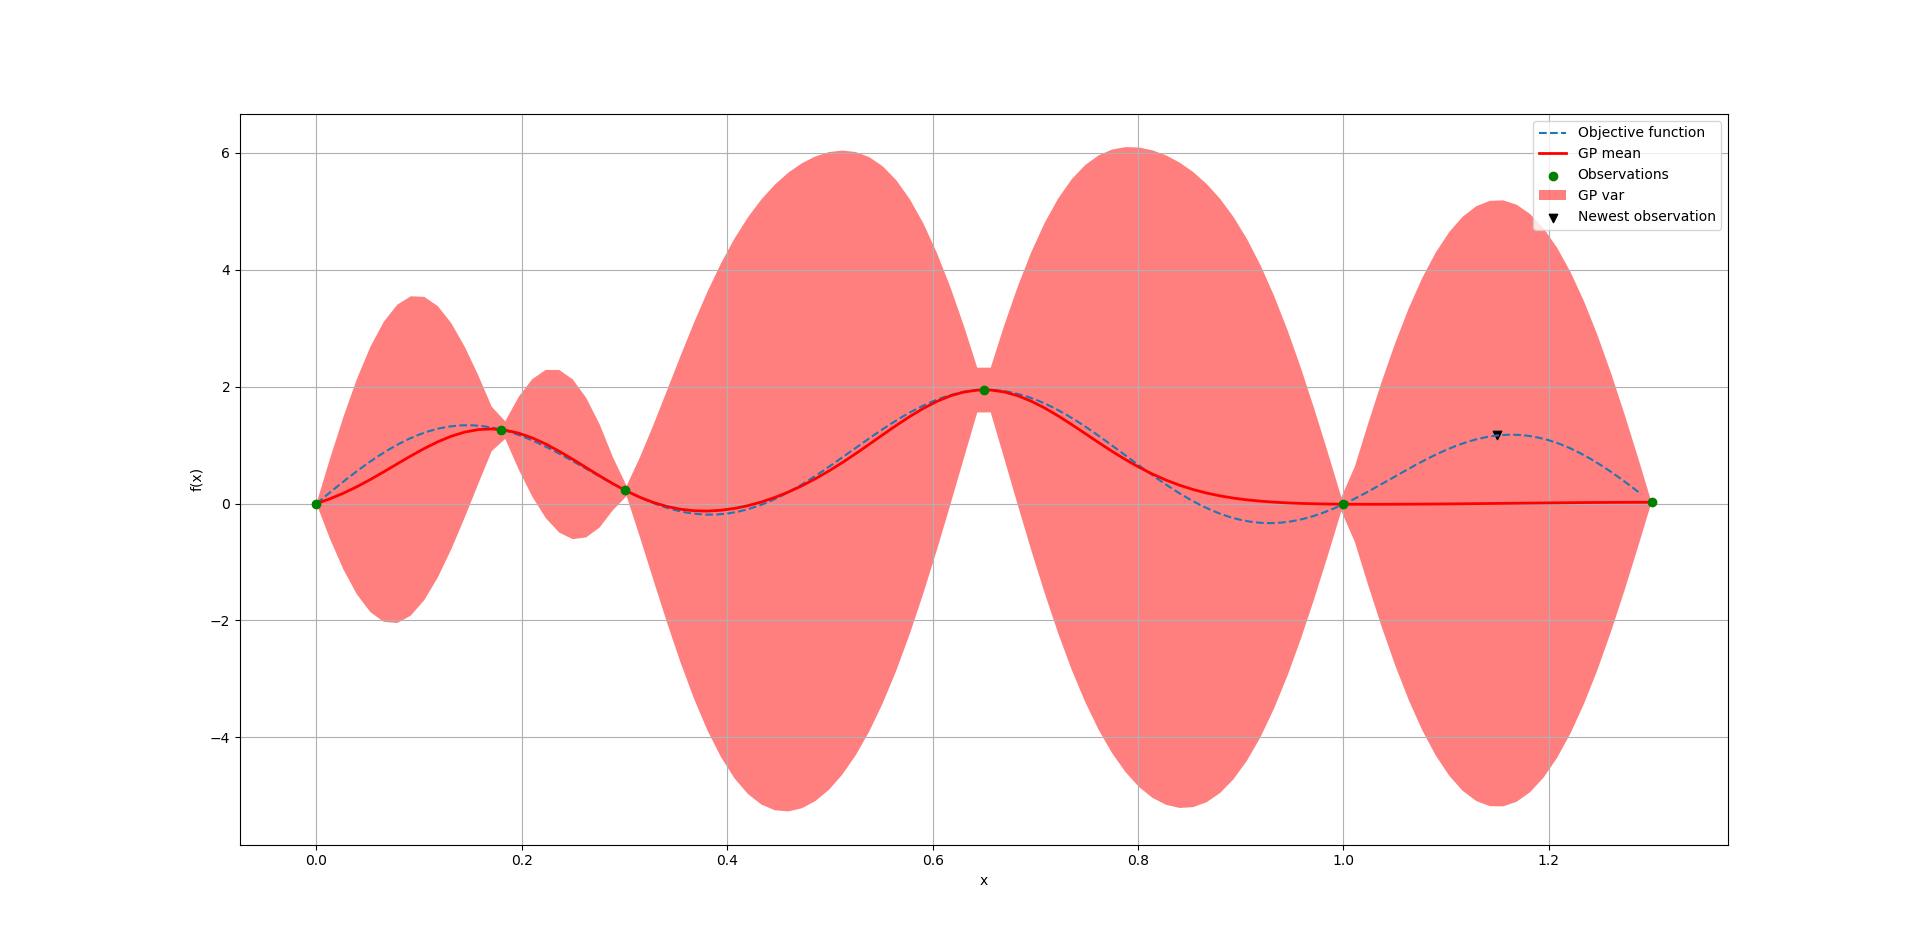
\includegraphics[width=\linewidth]{images/intro_images/BOLoop_4.png}}
%    \only<5>{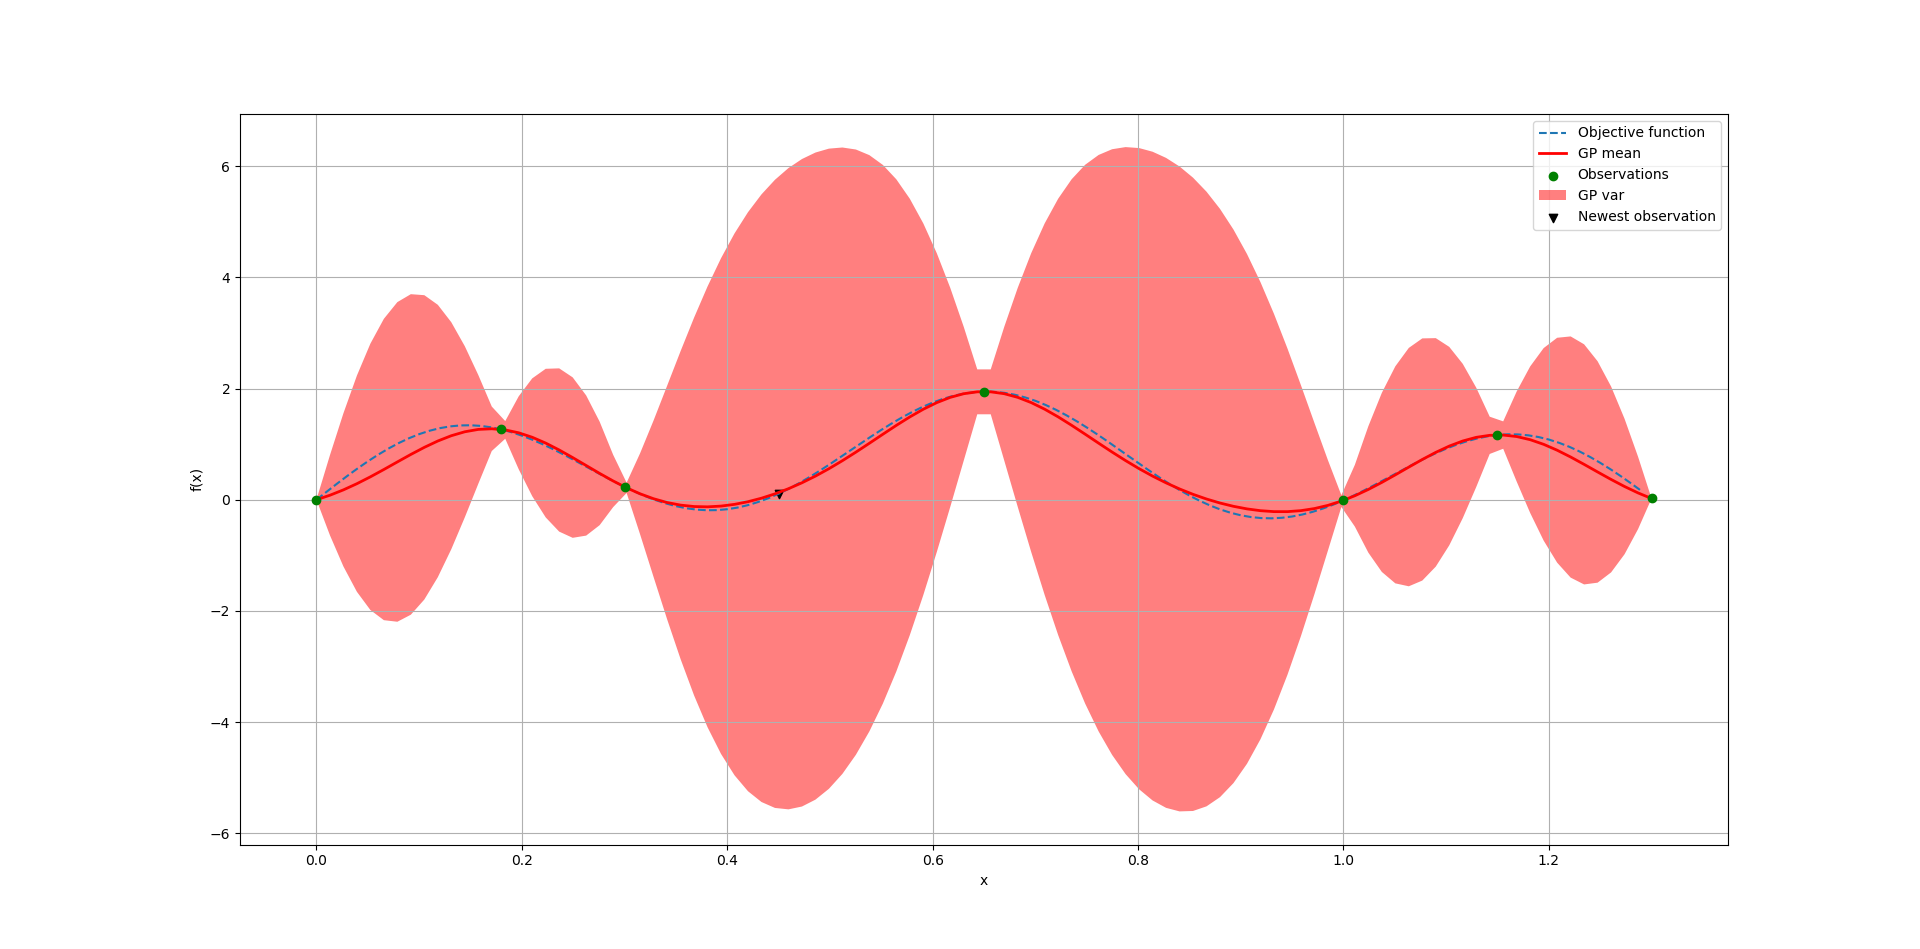
\includegraphics[width=\linewidth]{images/intro_images/BOLoop_5.png}}
%    \only<6>{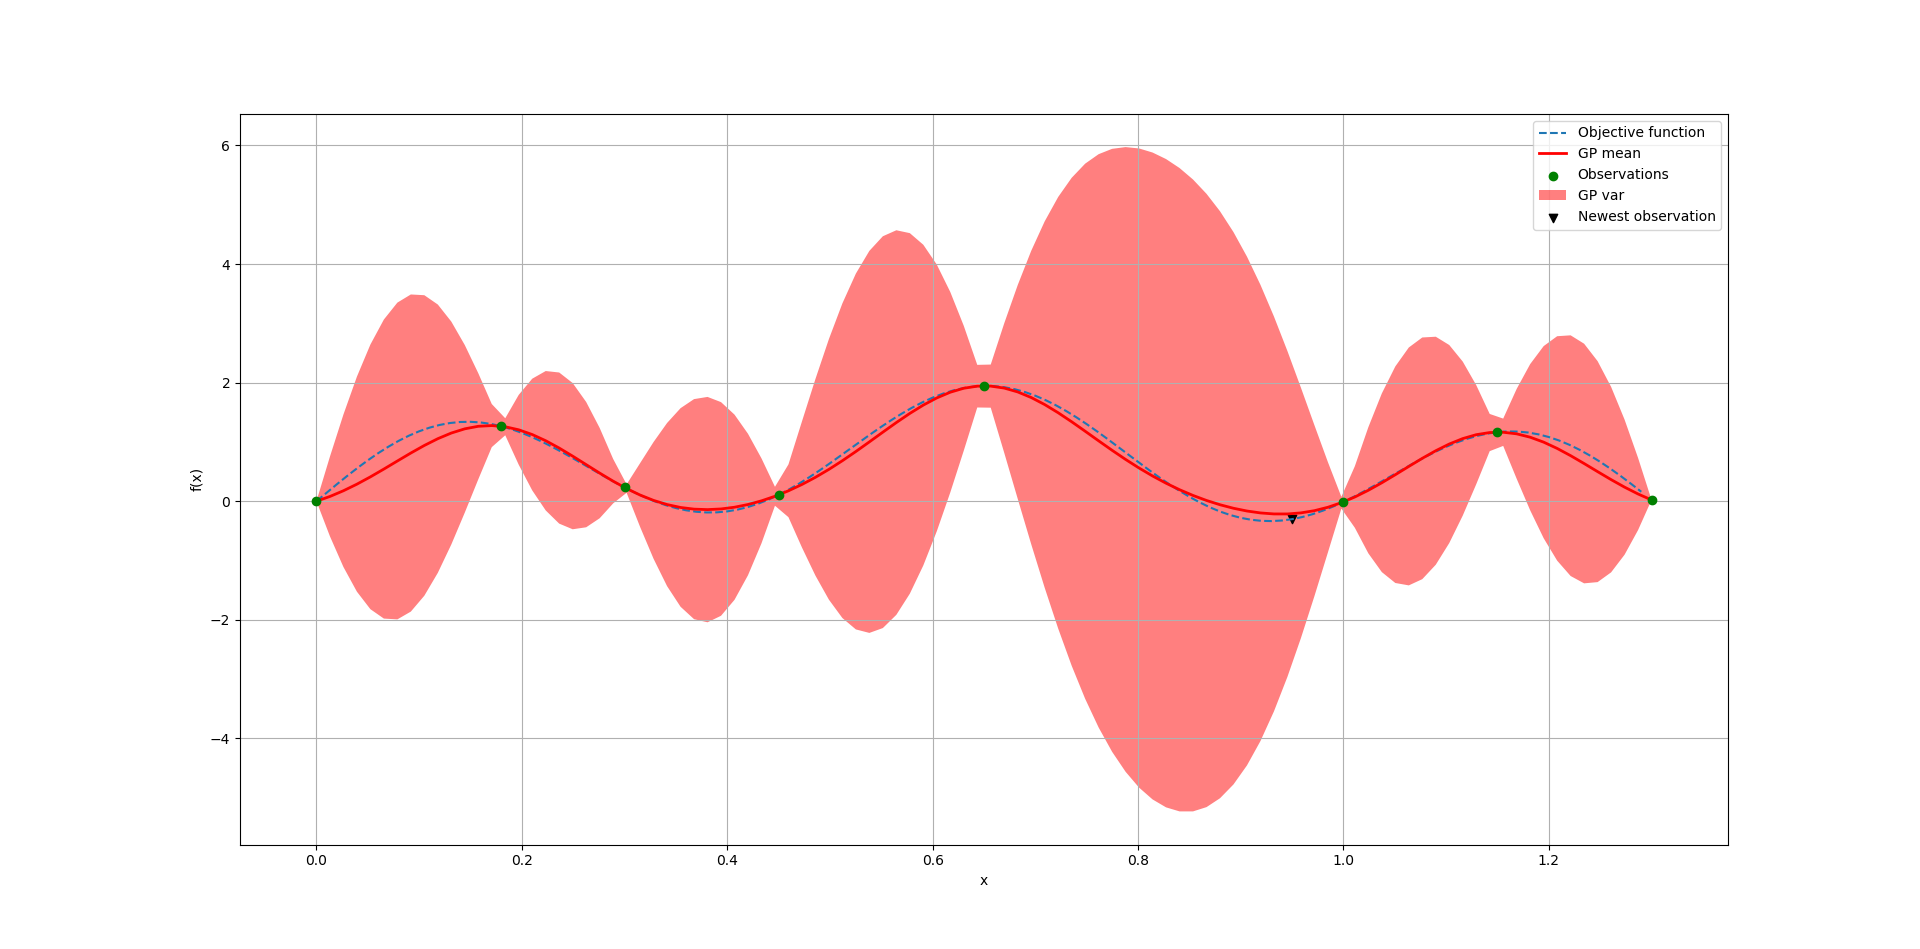
\includegraphics[width=\linewidth]{images/intro_images/BOLoop_6.png}}
%    \only<7>{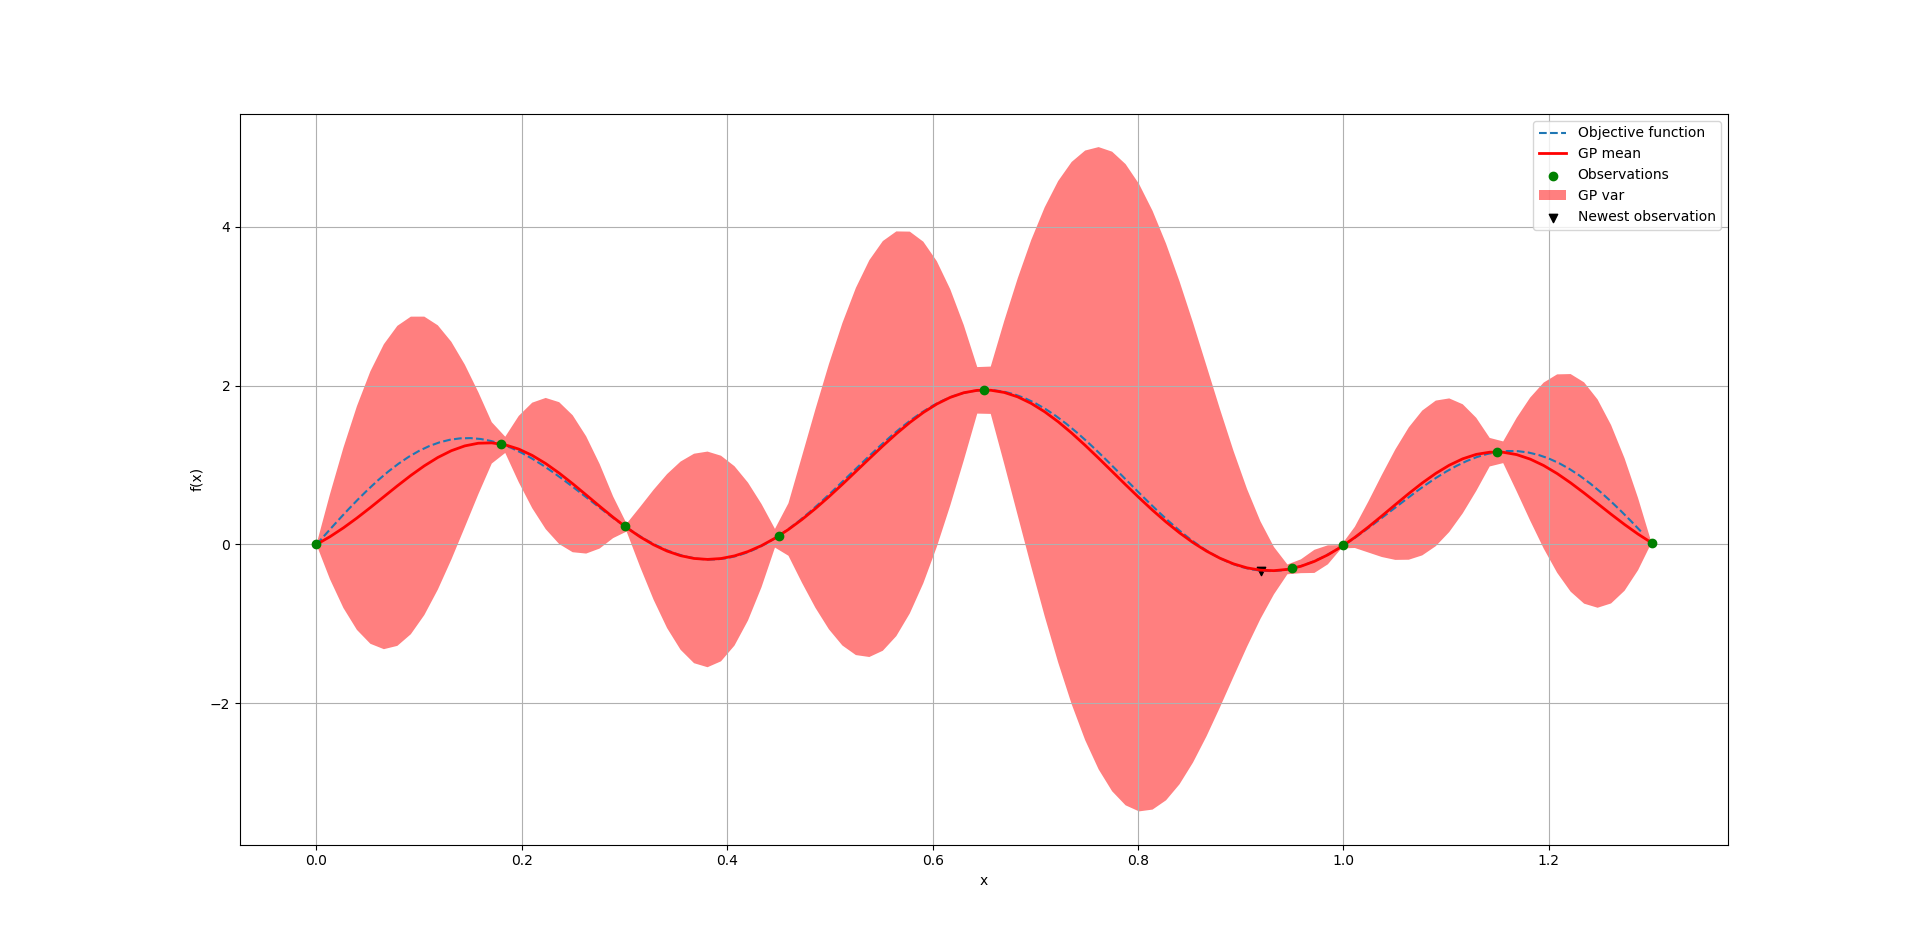
\includegraphics[width=\linewidth]{images/intro_images/BOLoop_7.png}}
%    \only<8>{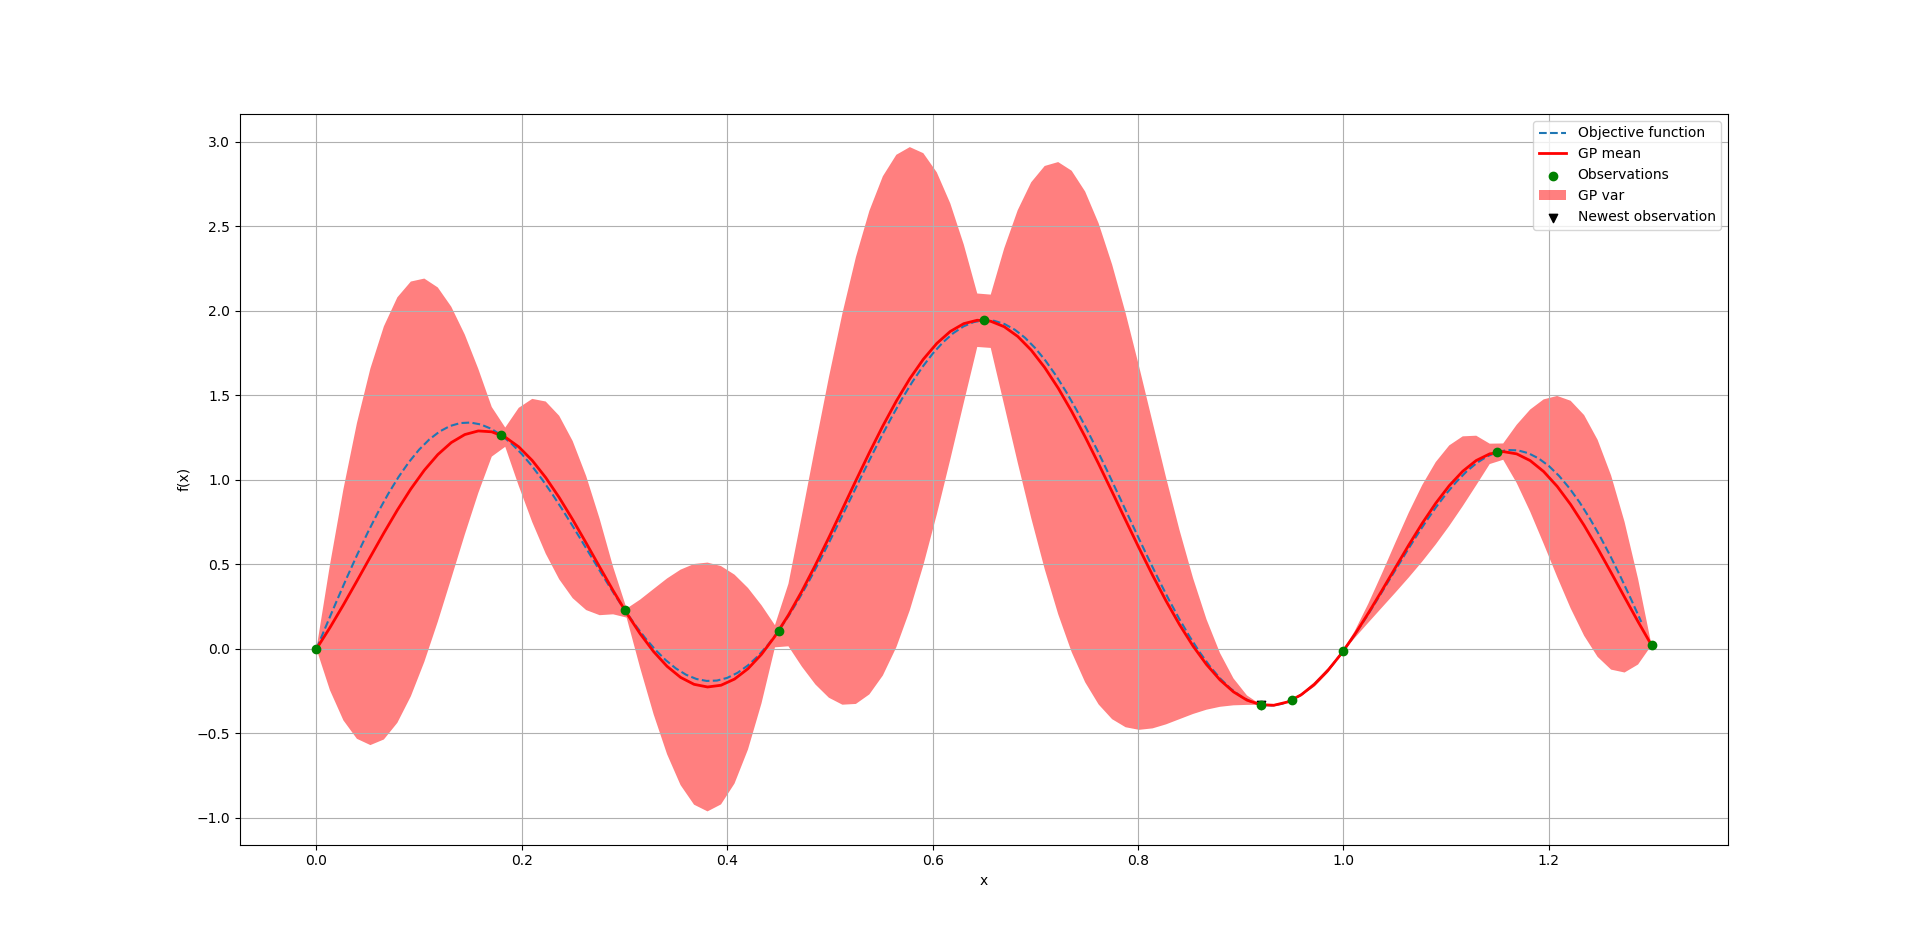
\includegraphics[width=\linewidth]{images/intro_images/BOLoop_8.png}}
%\end{figure}
%\end{frame}
%----------------------------------------------------------------------

\begin{frame}[c]{Bayesian Optimization: Pseudocode}

\begin{center}
\begin{minipage}{0.75\textwidth}
\begin{algorithm}[H]
    %\DontPrintSemicolon
%    \SetAlgoLined
    \setcounter{AlgoLine}{0}
    \SetKwInOut{Require}{Require}
    \SetKwInOut{Result}{Result}
    
    \Require{Search space $\pcs$, 
    		cost function $\cost$, 
    		acquisition function $\acq$, predictive model $\surro$,
    		maximal number of function evaluations $\bobudget$}
    \Result{Best configuration $\finconf$
    (according to $\dataset$ or 
    $\surro$)}
    
	Initialize data $\iter[0]{\dataset}$ with initial observations\;% \leftarrow \varnothing$\; 
	 
    \For{$\bocount=1$ \KwTo $\bobudget$}{
		%\While{$B$ not exhausted} {
		Fit predictive model $\iter[\bocount]{\surro}$ on $\iter[\bocount-1]{\dataset}$\;
		
		Select next query point: $\bonextsample \in \argmax_{\conf \in \pcs} \acq(\conf; \iter[\bocount-1]{\dataset}, \iter[\bocount]{\surro})$\;
		
		Query $\bonextobs$\;
		
		Update data: $\iter[\bocount]{\dataset} \leftarrow \iter[\bocount-1]{\dataset} \cup \{\langle \bonextsample, \bonextobs \rangle \}$\;
	}
	\caption*{BO loop}
\end{algorithm}
\end{minipage}
\end{center}
\end{frame}
%-----------------------------------------------------------------------
\begin{frame}[c]{Bayesian Optimization: Origin of the Name}

\begin{itemize}
    \item Bayesian optimization uses \alert{Bayes' theorem}: 
    	\begin{equation*}
    	    P(A \vert B) = \frac{P(B \vert A) \times  P(A)}{P(B)}
    	    \propto P(B \vert A) \times  P(A)
    	\end{equation*} 
    \item Bayesian optimization uses this to compute a posterior over functions: 
        \begin{equation*}
            P(\func \vert \dataset_{1:\bocount}) \propto P(\dataset_{1:\bocount} \vert \func) \times P(\func), \text{~~~~ where } \dataset_{1:\bocount} = \left \{ \conf_{1:\bocount}, \cost(\conf_{1:\bocount}) \right\}
        \end{equation*} 
\pause
\vspace*{-0.5cm}
    \item Meaning of the individual terms:
        \begin{itemize}
            \item $P(f)$ is the \alert{prior} over functions, which represents our belief about the space of possible objective functions \alert{before} we see any data
            \item $\dataset_{1:\bocount}$ is the \alert{data} (or observations, evidence)
            \item $P(\dataset_{1:\bocount} \vert \func)$ is the likelihood of the data given a function
            \item $P(\func \vert \dataset_{1:\bocount})$ is the \alert{posterior} probability over functions given the data
        \end{itemize}
    \end{itemize}
\end{frame}
%-----------------------------------------------------------------------
\begin{frame}[c]{Bayesian Optimization: Advantages and Disadvantages}

\begin{columns}[T] % align columns
\begin{column}{.48\textwidth}


\begin{block}{Advantages}
\begin{itemize}
  \item Sample efficient 
  \item Can handle noise
  \item Native incorporation of priors 
  \item Does not require gradients 
  \item Theoretical guarantees
\end{itemize}
\end{block}

\end{column}%

\hfill%
\pause 
\begin{column}{.48\textwidth}

\begin{block}{Disadvantages}
\begin{itemize}
  \item Overhead because of model training in each iteration 
  \item Crucially relies on robust surrogate model
  \item Inherently sequential (in its basic form)
\end{itemize}
\end{block}

\end{column}
\end{columns}

\end{frame}
%-----------------------------------------------------------------------
\begin{frame}[c]{Learning Goals of this Lecture}
\framesubtitle{After this lecture, students can ...}

\begin{itemize}
    \item Explain the basics of Bayesian optimization
    \item Derive \alert{simple acquisition functions}
    \item Describe \alert{advanced acquisition functions}
    \item Describe possible \alert{surrogate models} and their pros and cons 
    \item Discuss the \alert{limits of Bayesian optimization} and extensions to tackle these
%    \item Describe the \alert{alternative Bayesian optimization approach of TPE}
    \item Discuss \alert{success stories} of Bayesian optimization
\end{itemize}

\end{frame}

%-----------------------------------------------------------------------
%----------------------------------------------------------------------
%\begin{frame}[c]{Surrogate modelling}
%\framesubtitle{General idea}
%\begin{itemize}
%    \item Use a surrogate model of the expensive function $\cost$ as a cheap-to-evaluate proxy.
%    \begin{itemize}
%        \item Use a probabilistic model with well-calibrated uncertainty predictions.
%    \end{itemize}
%    \pause
%    \item Define a utility function to guide the search for new data points.
%    \pause
%    \item Use the optimization of the utility function as a decision procedure to provide inference on where to evaluate next.
%
%\end{itemize}
%\end{frame}

%-----------------------------------------------------------------------

%\end{document}
    \section{Bayesian Optimization}
%----------------------------------------------------------------------
%----------------------------------------------------------------------
\begin{frame}[c]{Bayesian Optimization: Bayes rule}

\begin{itemize}
    \item Let $A$ and $B$ be two events with $P(B) \neq 0$ \pause
    \item The conditional probability of $A$ given $B$ is defined to be:
	\begin{equation*}
	    P(A \vert B) = \frac{P(A \cap B)}{P(B)}
    \label{eq:cond_prob}  
	\end{equation*} \pause
	\item One can rearrange the terms to show:
        \begin{equation*}
            P(A \cap B) = P(A \vert B) * P(B)
        \end{equation*} \pause
\end{itemize}

\begin{center}
\begin{minipage}{0.75\textwidth}
\begin{block}{Bayes rule (theorem)}
Since $A \cap B = B \cap A$, one can rewrite above relation as:
	\begin{equation*}
	    P(A \vert B) = \frac{P(B \vert A) * P(A)}{P(B)}
        \label{eq:bayes_rule}  
	\end{equation*}
\end{block}
\end{minipage}
\end{center}

\end{frame}
%-----------------------------------------------------------------------

%----------------------------------------------------------------------
%----------------------------------------------------------------------
\begin{frame}[c]{Bayesian Optimization: Bayes rule - example}

\begin{block}{Bayes rule - example}
    You are planning a picnic today, but the morning is cloudy: \pause
    \begin{itemize}
        \item 50\% of all rainy days start off cloudy, \pause
        \item cloudy mornings are common (about 40\% of days start cloudy), \pause
        \item it is a dry month (only 3 of 30 days tend to be rainy, or 10\%). \pause
    \end{itemize}
    
    \emph{What is the chance of rain during the day?}
\end{block}

 \pause

\begin{block}{Bayes rule - solution}
	\begin{equation*}
	\begin{aligned}
	    P(RainyDay \vert CloudyMorning) = \frac{P(CloudyMorning \vert RainyDay) * P(RainyDay)}{P(CloudyMorning)} \\  \pause
	    P(RainyDay \vert CloudyMorning) = \frac{0.5 * 0.1}{0.4} = 0.125
	\end{aligned}
	\end{equation*}
\end{block}

\note[item]{source: https://www.mathsisfun.com/data/bayes-theorem.html}
\note[item]{https://www.countbayesie.com/blog/2015/2/18/bayes-theorem-with-lego}
        
\end{frame}
%-----------------------------------------------------------------------

%----------------------------------------------------------------------
%----------------------------------------------------------------------
\begin{frame}[c]{Bayesian Optimization: Where does the name come from?}

\begin{itemize}
    \item Bayesian optimization uses Bayes' theorem in a form: 
    	\begin{equation*}
    	    P(A \vert B) \propto P(B \vert A) * P(A)
    	\end{equation*} \pause
    \item We refer to:
        \begin{itemize}
            \item $A$ as a model (or hypothesis, theory), \pause
            \item $B$ as a data (or observations, evidence),\pause
            \item $P(A \vert B)$ as a \emph{posterior} probability of a model given a data,\pause
            \item $P(B \vert A)$ as a \emph{likelihood} of a data given a model, \pause
            \item $P(A)$ as a \emph{prior} probability of a model, which represents our belief about the space of possible objective functions. \pause
        \end{itemize}
    \item In our application:
        \begin{equation*}
            P(\func \vert \dataset_{1:\bocount}) \propto P(\dataset_{1:\bocount} \vert \func) * P(\func)
        \end{equation*} \pause
        where $\dataset_{1:\bocount} = \left \{ \conf_{1:\bocount}, \func(\conf_{1:\bocount}) \right \}$.

\end{itemize}

        
\end{frame}
%-----------------------------------------------------------------------

%----------------------------------------------------------------------
%----------------------------------------------------------------------
\begin{frame}[c]{Bayesian Optimization: Pseudocode}
\begin{center}
\begin{minipage}{0.75\textwidth}
\begin{algorithm}[H]
    \Input{Search Space $\pcs$, 
    		black box function $\func$, 
    		acquisition function $\acq$, \\
    		maximal number of function evaluations $\bobudget$.
    	}
	\BlankLine
	$\dataset_0$ $\leftarrow$ initial\_design($\pcs$); 
	
	\For{\bocount = $1, 2, \ldots \bobudget - |\dataset_0|$}{
		%\While{$B$ not exhausted} {
		$\surro$ $\leftarrow$ fit predictive model on $\dataset_{\bocount-1}$;
		
		select $\bonextsample$ by optimizing $\bonextsample \in \argmax_{\conf \in \pcs} \acq(\conf; \dataset_{\bocount-1}, \surro)$;
		
		Query $\bonextobs := \func(\bonextsample)$;
		
		Add observation to data $\dataset_{\bocount} := \dataset_{\bocount-1} \cup \{\langle \bonextsample, \bonextobs \rangle \}$;\\
	}
	\Return{Best $\conf$ according to $\dataset_\bocount$ or $\surro$}
	\caption{BO loop}
\end{algorithm}
\end{minipage}
\end{center}
\note[item]{how to end lines?}
\end{frame}
%-----------------------------------------------------------------------

%-----------------------------------------------------------------------
%-----------------------------------------------------------------------
\begin{frame}[c]{Bayesian Optimization: Summary}

\begin{columns}[T] % align columns
\begin{column}{.48\textwidth}

\only<1-9>{
    \begin{block}{Advantages}
    \begin{itemize}
      \item Sample efficient \pause
      \item Native incorporation of priors \pause
      \item Does not require local gradients nor Hessian approximations \pause
      \item ...
    \end{itemize}
    \end{block}
}
\end{column}%

\pause
\hfill%

\begin{column}{.48\textwidth}
\only<4-9>{
    \begin{block}{Disadvantages}
    \begin{itemize}
      \item Overhead because of model training in each iteration \pause
      \item Inherently sequential algorithm \pause
      \item Requires good choice of surrogate model \pause
      \item Requires good choice of acquisition function \pause
      \item Has hyperparameter on its own
    \end{itemize}
\end{block}
}
\end{column}
\end{columns}


\end{frame}
%-----------------------------------------------------------------------
    \section{Acquisition Functions}
%----------------------------------------------------------------------
%----------------------------------------------------------------------
\begin{frame}[c]{Acquisition Functions}
\framesubtitle{Description}
\comment{Refine, maybe consult a tutorial.}
\begin{itemize}
    \item \cemph{red}{Problem:} Given the surrogate function $\iter{\surro}(\conf)$ at the $\bocount\,$th iteration of BO, choose the "best" candidate $\iter{\conf}\in \pcs$ to evaluate $\cost(\conf)$ at next.
    \pause
    \item \cemph{violet}{Solution(?):} Evaluate at a global optimum of $\iter{\surro}(\conf)$ (in our discussion, minimum) - in the case of GPs, say, a global optimum of the mean function.
    \pause
    \item \cemph{red}{Issues:}
    \begin{itemize}
        \pause
        \item The surrogate function is inaccurate. The global optimum of $\iter{\surro}(\conf)$ is not necessarily the "best" candidate for evaluating $\cost(\conf)$ at. This is exactly why every candidate $\conf$ has an assosciated variance $\variance(\conf)$.
        \pause
        \item When the actual underlying distribution is unknown, we also need to consider the exploration-exploitation trade-off.
    \end{itemize}
    \pause
    \item \cemph{blue}{Real Solution}: Generate a heuristic estimate $\acq(\cdot)$ aka Acquisition Function!
\end{itemize}

\end{frame}
%-----------------------------------------------------------------------
\begin{frame}[c]{Acquisition Functions}
\framesubtitle{Types}
\begin{itemize}
    \item Basic Acquisition Functions
    \begin{itemize}
        \item Probability of Improvement - PI
        \item Expected Improvement - EI
        \item Lower/Upper Confidence Bounds - LCB/UCB
        \item Thompson Sampling - TS
    \end{itemize}
    \item Advanced Acquisition Functions
    \begin{itemize}
        \item Knowledge Gradient
        \item Entropy Search
    \end{itemize}
\end{itemize}

\end{frame}
%-----------------------------------------------------------------------
\subsection{Basic Acquisition Functions}
\begin{frame}[c]{Basic Acquisition Functions - PI}
\framesubtitle{Probability of Improvement - Concept}
\pause
\begin{figure}
  \centering
  \begin{tikzpicture}
    \node<+> (img1) {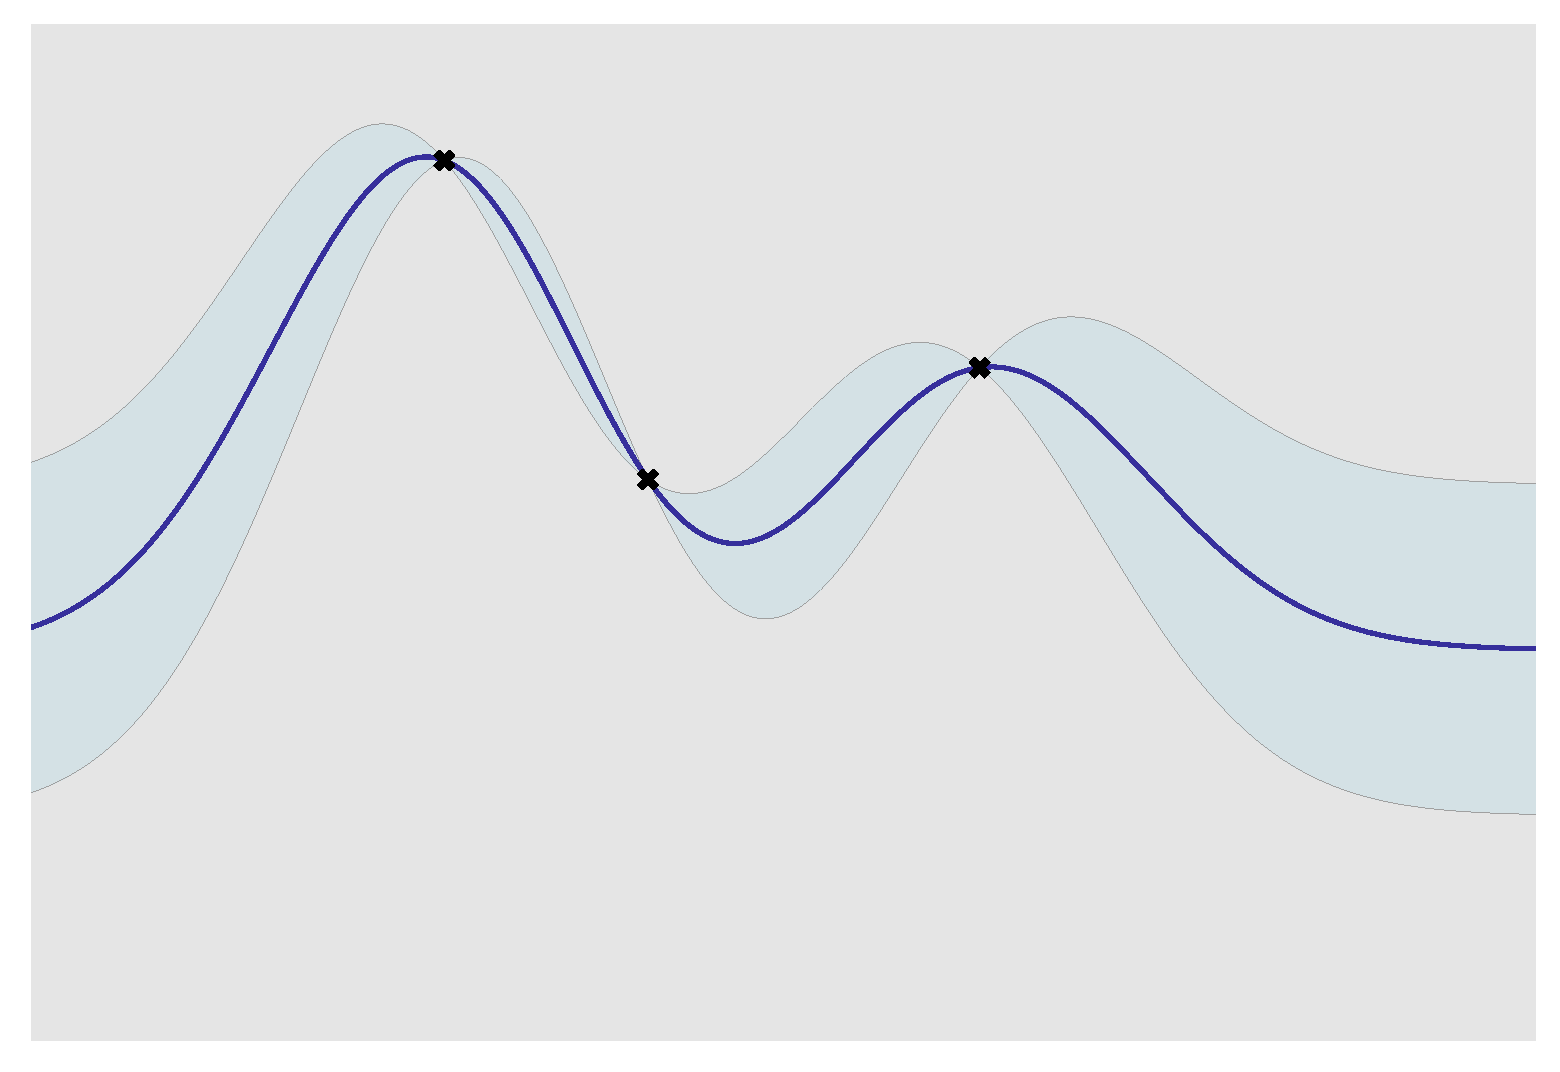
\includegraphics[width=.7\linewidth, height=0.7\textheight, keepaspectratio=true]{w06_hpo_bo/images/acq_func_images/pi_1.pdf}};
    \node<.> [below=0.01\belowcaptionskip of img1, align=center]{GP fit on 3 observations};

    \node<+> (img2) {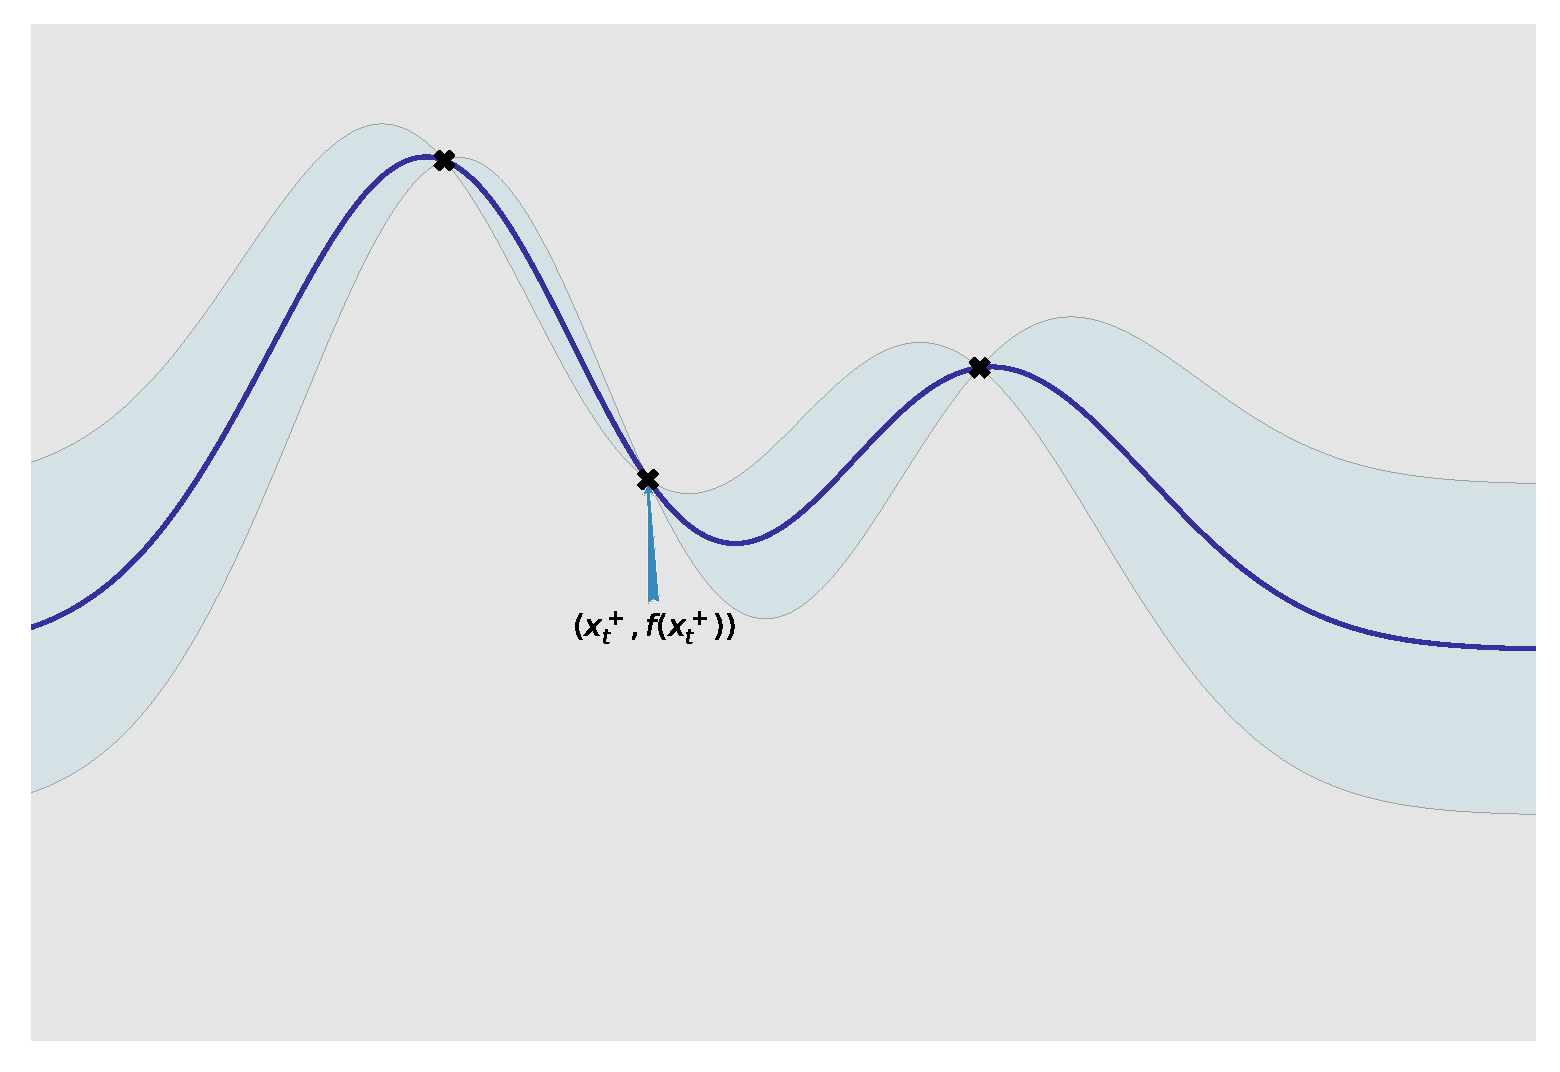
\includegraphics[width=.7\linewidth, height=0.7\textheight, keepaspectratio=true]{w06_hpo_bo/images/acq_func_images/pi_2.pdf}};
    \node<.> [below=0.01\belowcaptionskip of img2, align=center]{Current incumbent $\incumbent[\bocount-1]$ and it's observed value $\cost(\incumbent[\bocount-1])$};

    \node<+> (img3) {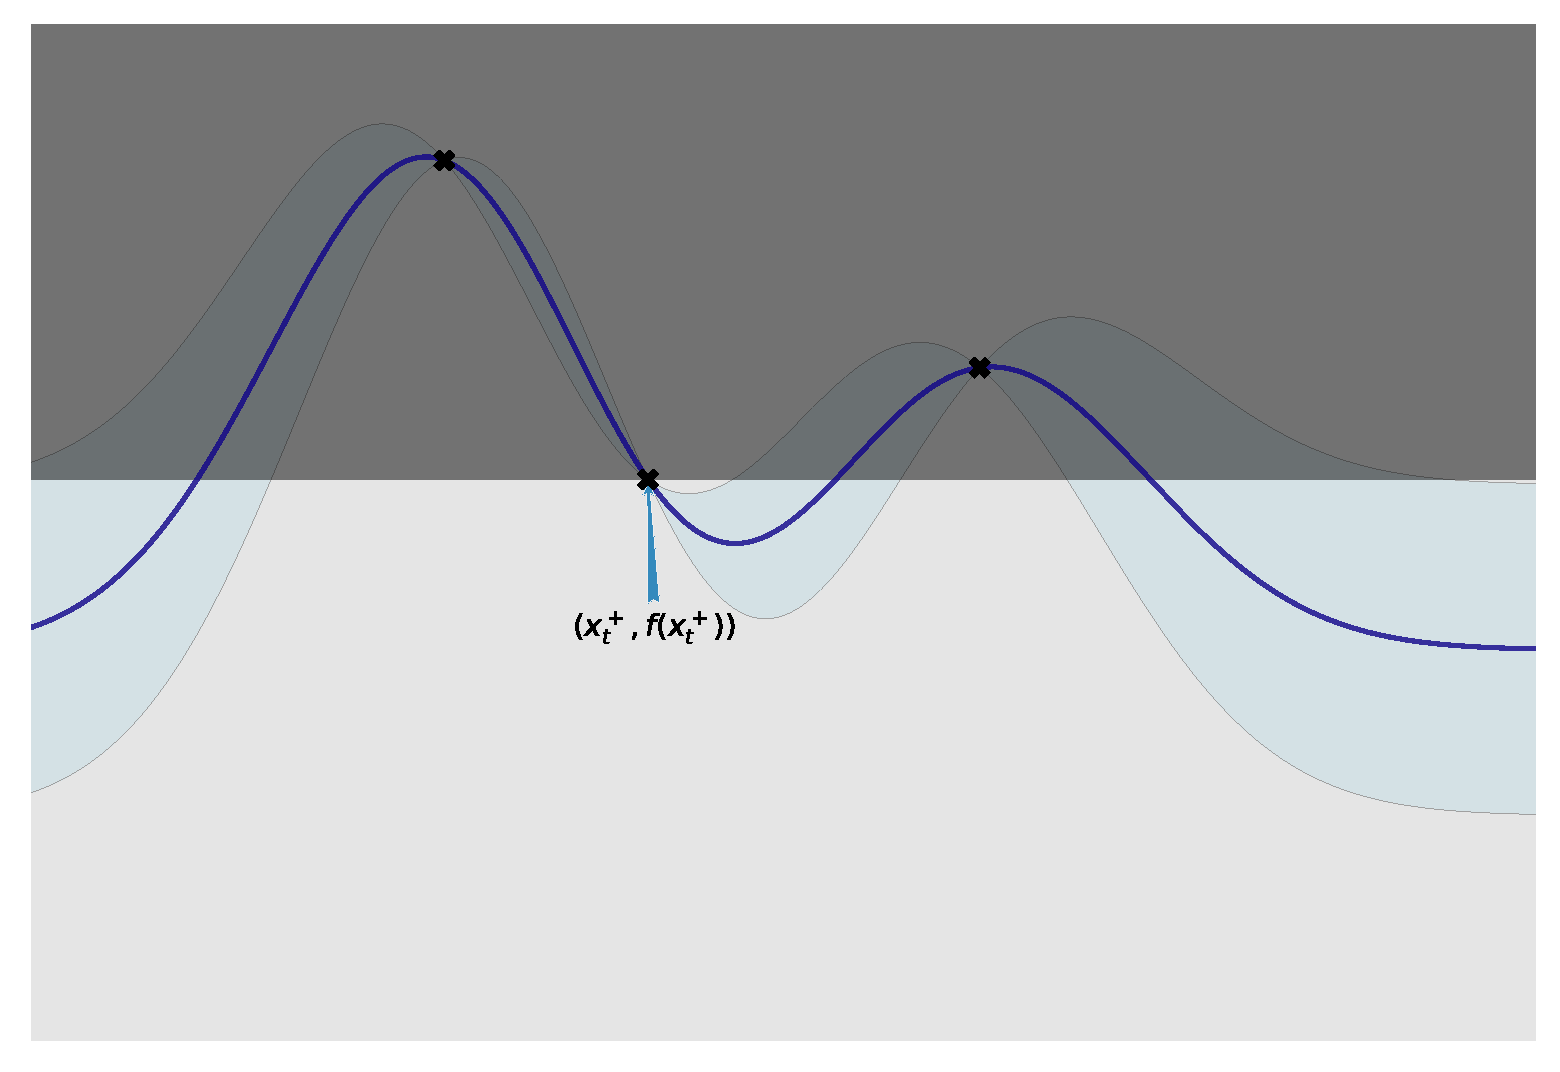
\includegraphics[width=.7\linewidth, height=0.7\textheight, keepaspectratio=true]{w06_hpo_bo/images/acq_func_images/pi_3.pdf}};
    \node<.> [below=0.01\belowcaptionskip of img3, align=center]{Region of probable improvement};

    \node<+> (img4) {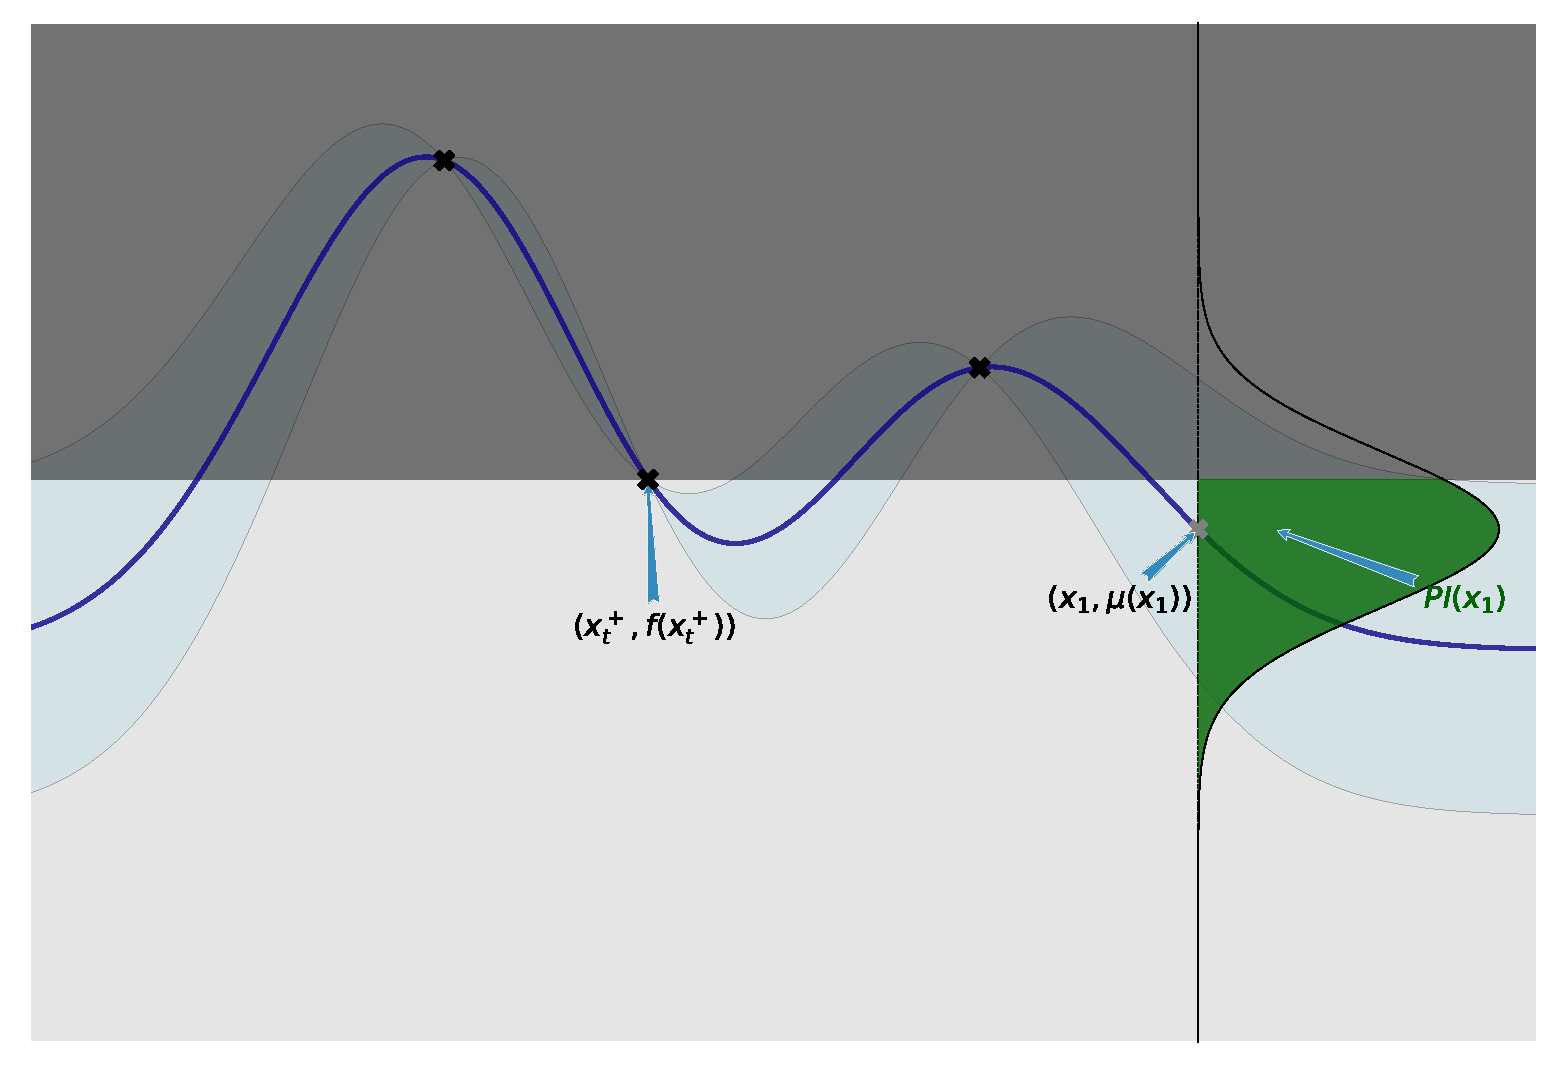
\includegraphics[width=.7\linewidth, height=0.7\textheight, keepaspectratio=true]{w06_hpo_bo/images/acq_func_images/pi_4.pdf}};
    \node<.> [below=0.01\belowcaptionskip of img4, align=center]{PDF of a good candidate parameter value};

    \node<+> (img5) {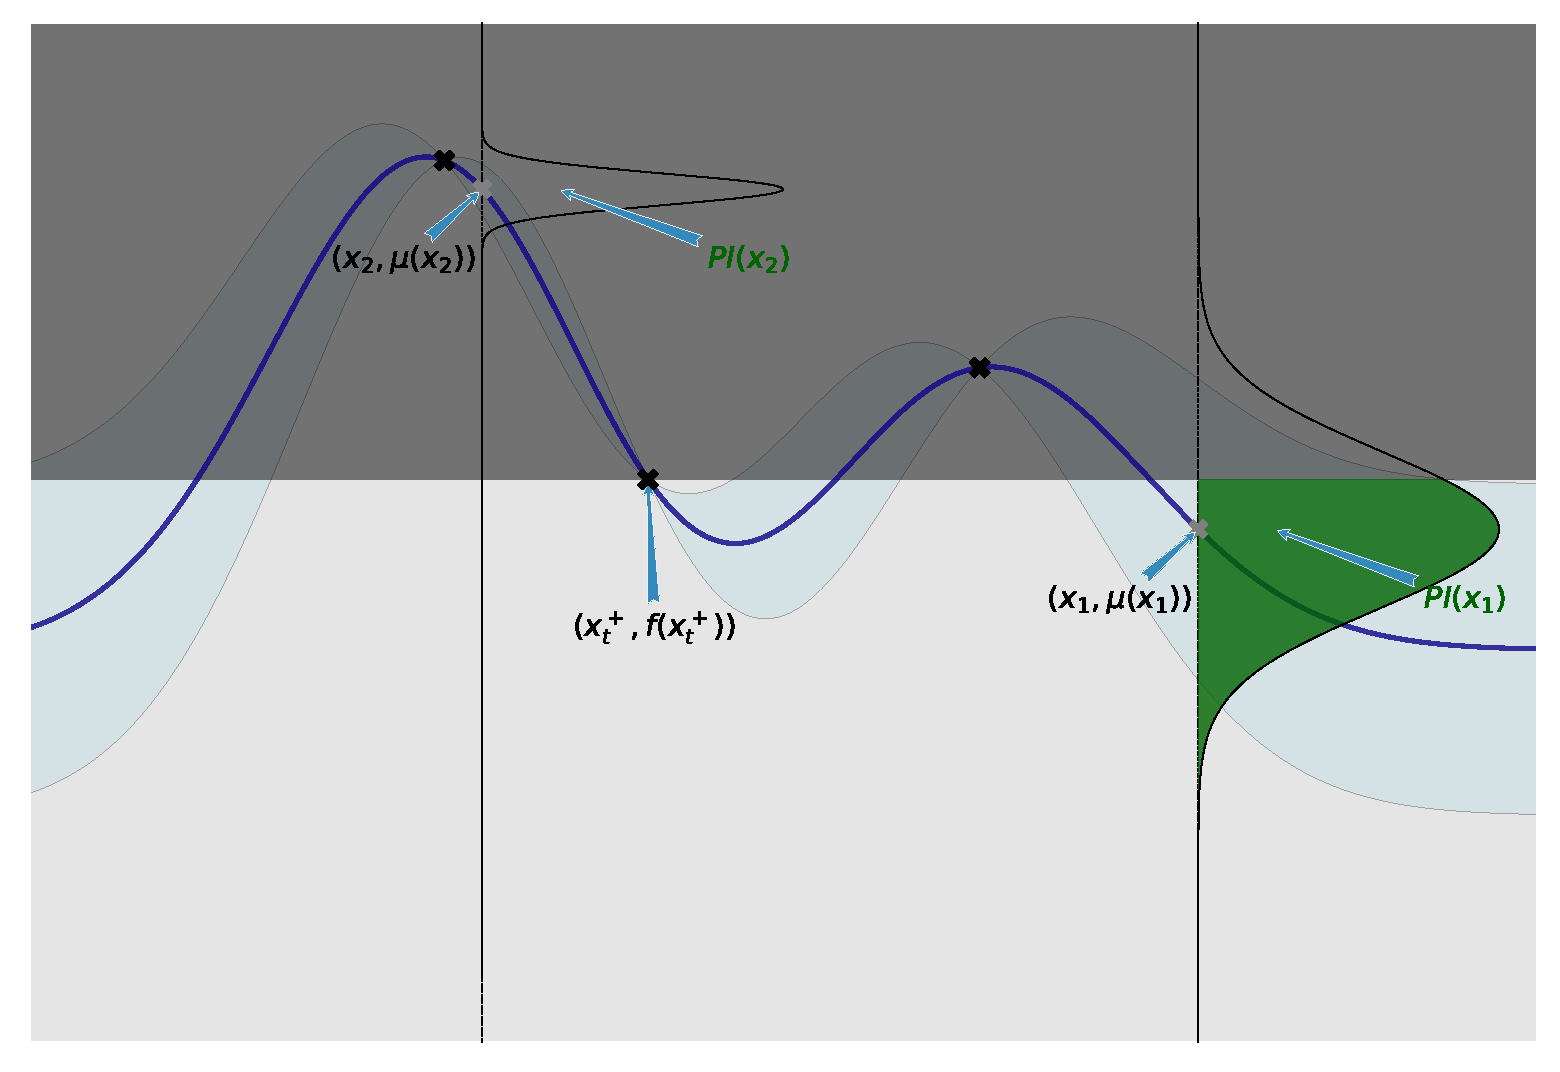
\includegraphics[width=.7\linewidth, height=0.7\textheight, keepaspectratio=true]{w06_hpo_bo/images/acq_func_images/pi_5.pdf}};
    \node<.> [below=0.01\belowcaptionskip of img5, align=center]{PDF of a bad candidate parameter value};
  \end{tikzpicture}
\end{figure}

\end{frame}
%-----------------------------------------------------------------------
\begin{frame}[c]{Basic Acquisition Functions - PI}
\framesubtitle{Probability of Improvement - Choosing a candidate}
\pause \comment{Verify if definitions suit minimization!}
\begin{itemize}
    \item[]
        \[
            \iter{PI}(\conf) = P(\cost(\conf) \leq \cost(\incumbent[\bocount-1])), \quad\incumbent[\bocount-1]\in\argmin_{\conf'\in\iter[\bocount-1]{\dataset}}\boobs\in\iter[\bocount-1]{\dataset}
        \]
    \newline
    where $P(\cdot)$ is the probability of an event.
    \pause
    \item[]
    \begin{align*}
        \iter{PI}(\conf) &= \cdf[Z] \\
        Z &= \dfrac{\cost(\incumbent[\bocount-1]) - \iter[\bocount-1]{\mean}(\conf) - \xi}{\iter[\bocount-1]{\stddev}(\conf)}
    \end{align*}
    \newline
    where $\cdf(\cdot)$ is the CDF of the standard normal distribution and $\xi$ is an exploration parameter.
    \pause
    \item[] \[\boxed{\bonextsample \in \argmax_{\conf\in\pcs}(\iter{PI}(\conf))}\]
%    \comment{Source: Tutorial by Brochu et al.: https://arxiv.org/pdf/1012.2599.pdf }
\end{itemize}
\end{frame}
%-----------------------------------------------------------------------
% \begin{frame}[c]{Basic Acquisition Functions - PI}
% \framesubtitle{Probability of Improvement - Features}
% \comment{To be replaced with a table of comparative features.}
% \begin{itemize}
%     \item Pure, greedy exploitation.
%     \item Intuitive.
%     \item Many known modes of failure.
% \end{itemize}
% \end{frame}
%-----------------------------------------------------------------------
\begin{frame}[c]{Basic Acquisition Functions - EI}
\framesubtitle{Expected Improvement - Concept}

\begin{figure}
  \centering
  \begin{tikzpicture}
    \node<+> (img1) {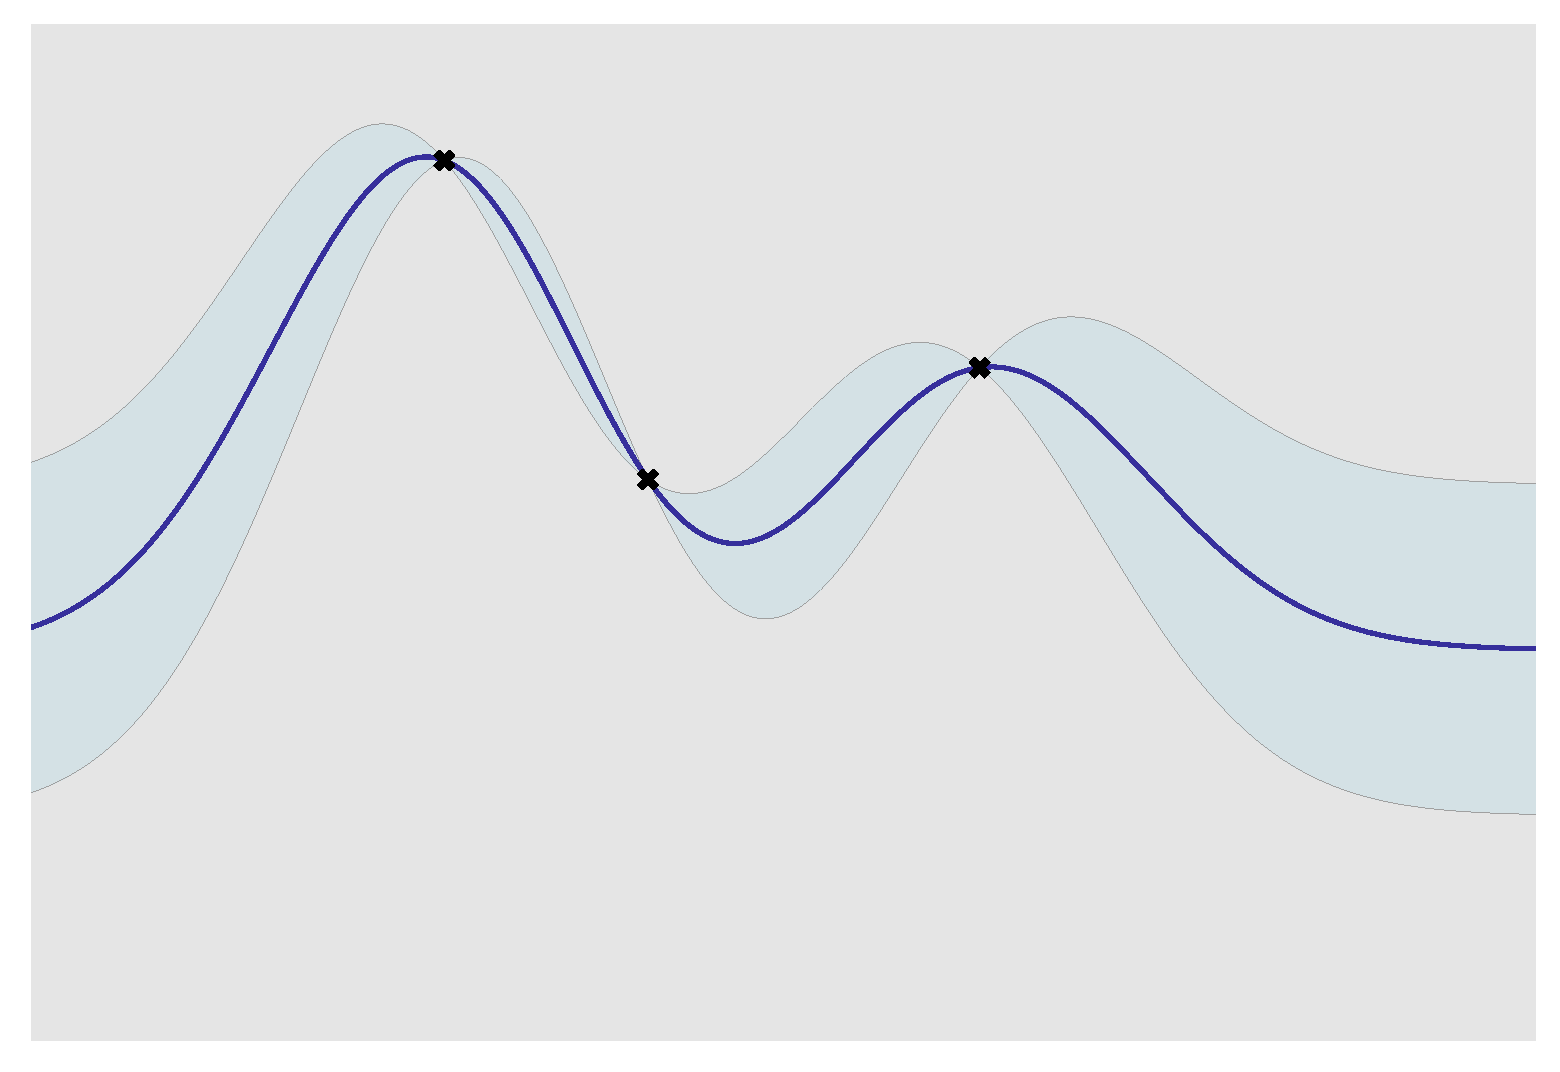
\includegraphics[width=.7\linewidth, height=0.7\textheight, keepaspectratio=true]{w06_hpo_bo/images/acq_func_images/ei_1.pdf}};
    \node<.> [below=0.01\belowcaptionskip of img1, align=center]{GP fit on 3 observations};

    \node<+> (img2) {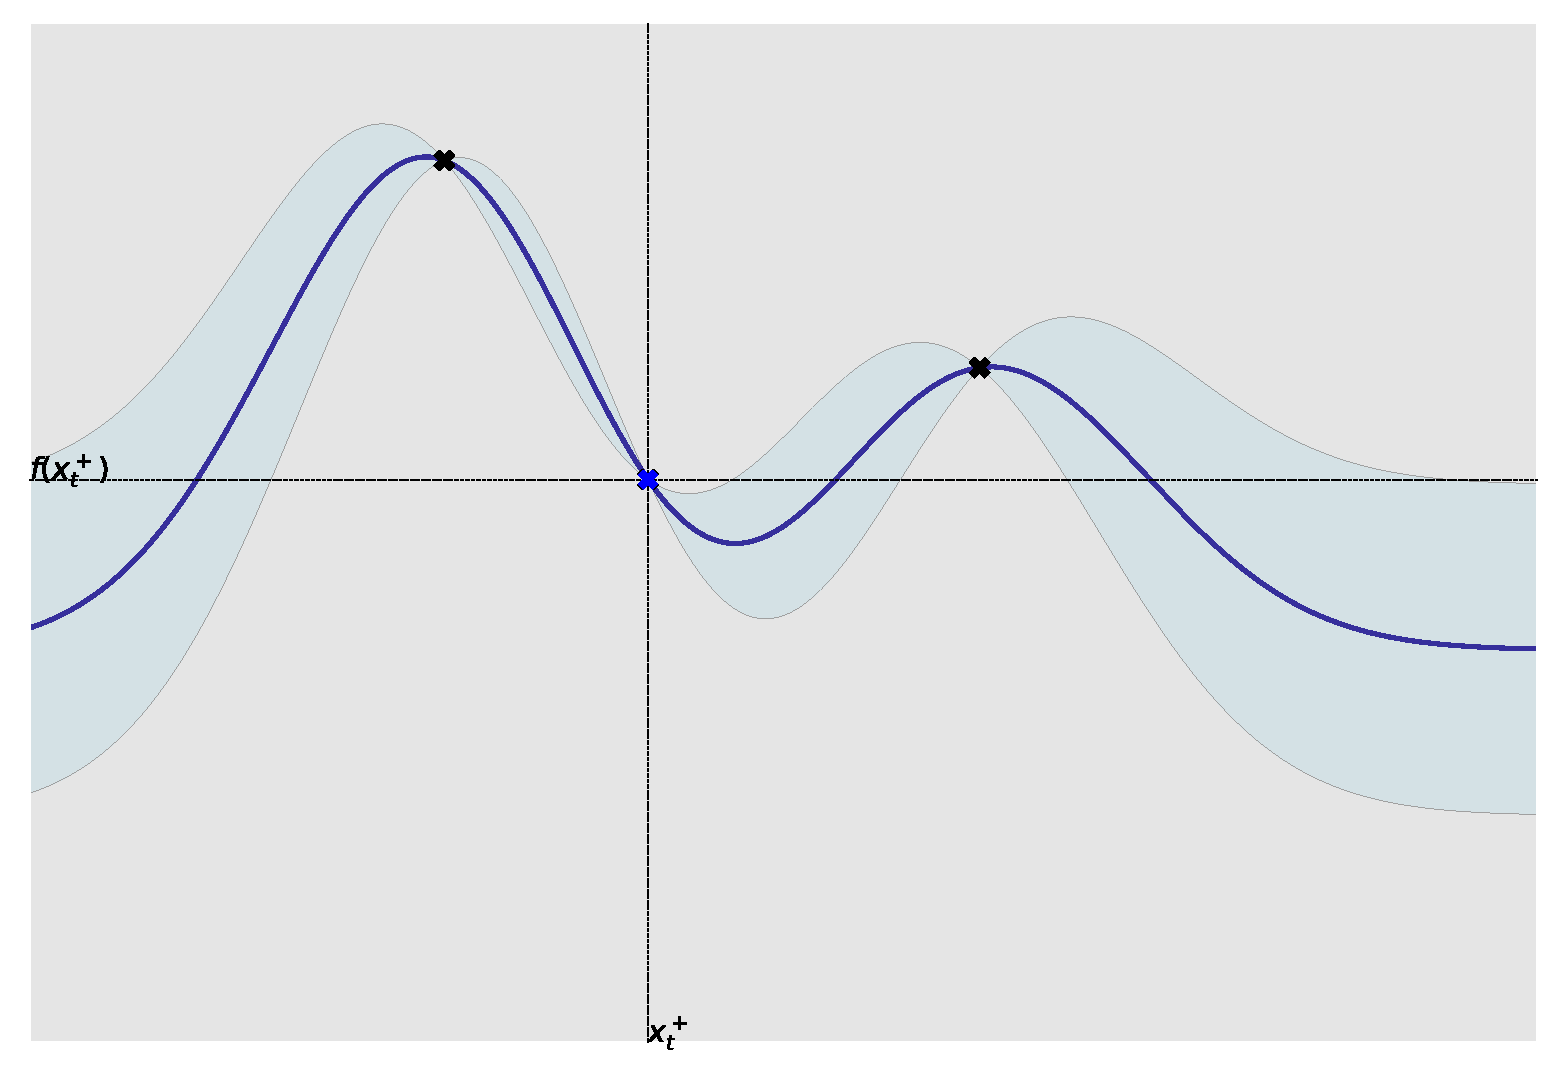
\includegraphics[width=.7\linewidth, height=0.7\textheight, keepaspectratio=true]{w06_hpo_bo/images/acq_func_images/ei_2.pdf}};
    \node<.> [below=0.01\belowcaptionskip of img2, align=center]{Current incumbent $\incumbent[\bocount-1]$ and its observed value $\cost(\incumbent[\bocount-1])$.};

    \node<+> (img3) {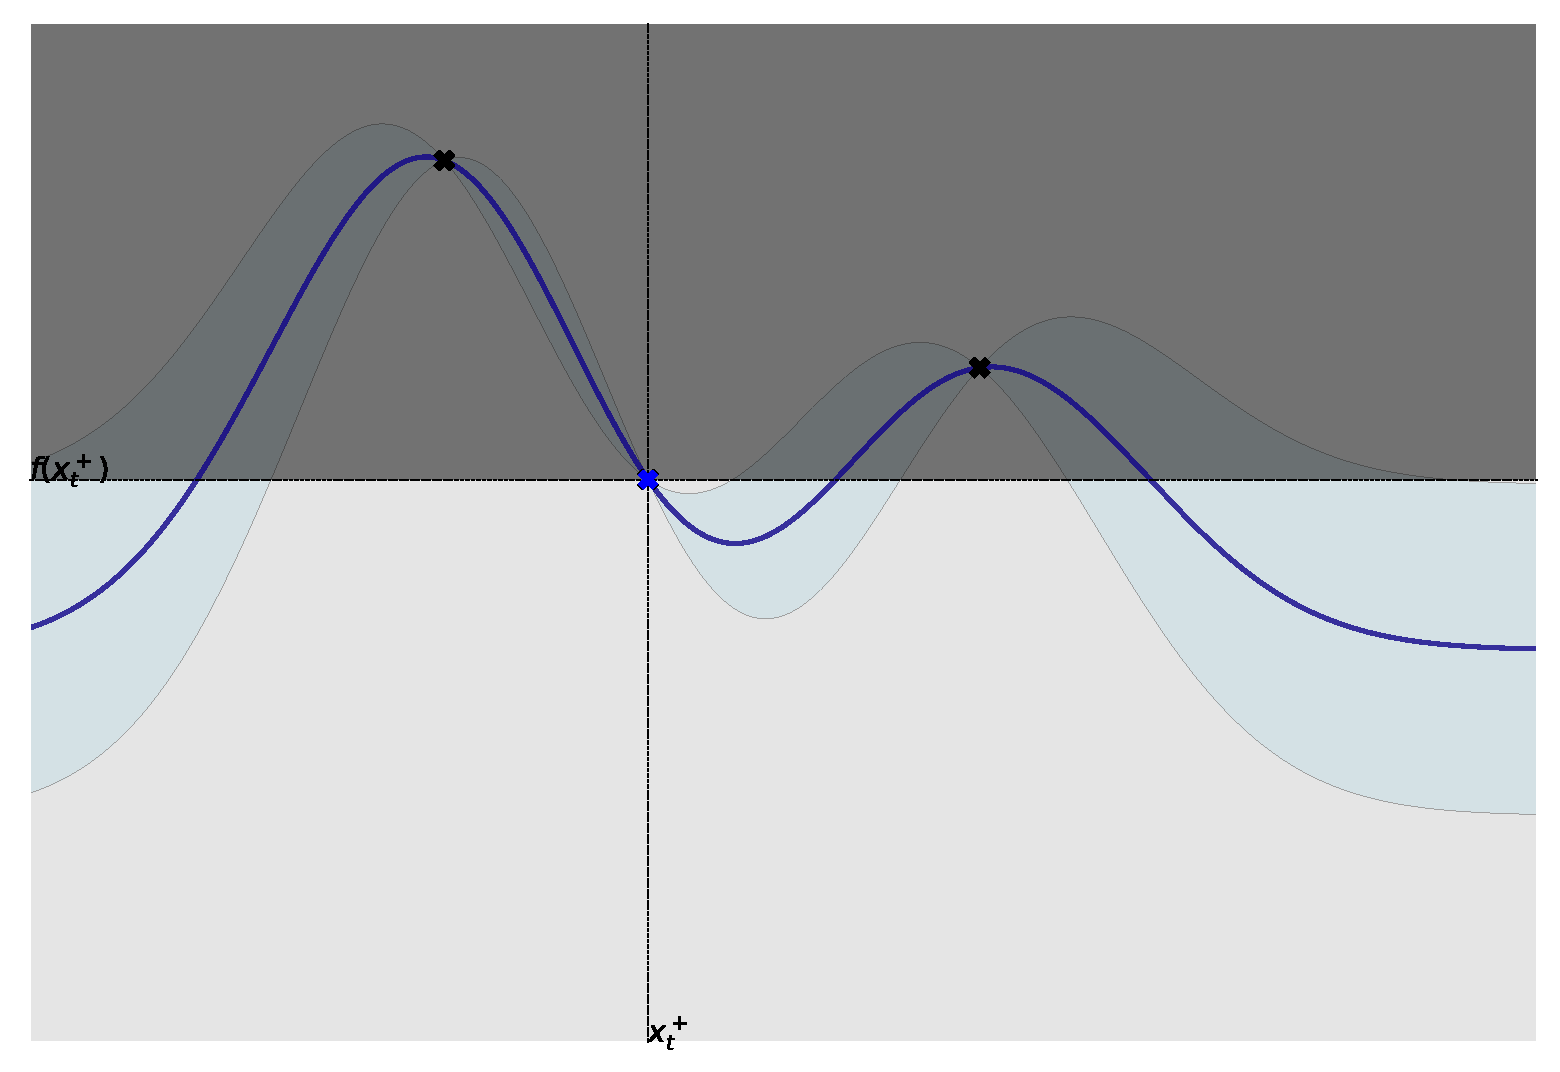
\includegraphics[width=.7\linewidth, height=0.7\textheight, keepaspectratio=true]{w06_hpo_bo/images/acq_func_images/ei_3.pdf}};
    \node<.> [below=0.01\belowcaptionskip of img3, align=center]{Zone of probable improvement};

    \node<+> (img4) {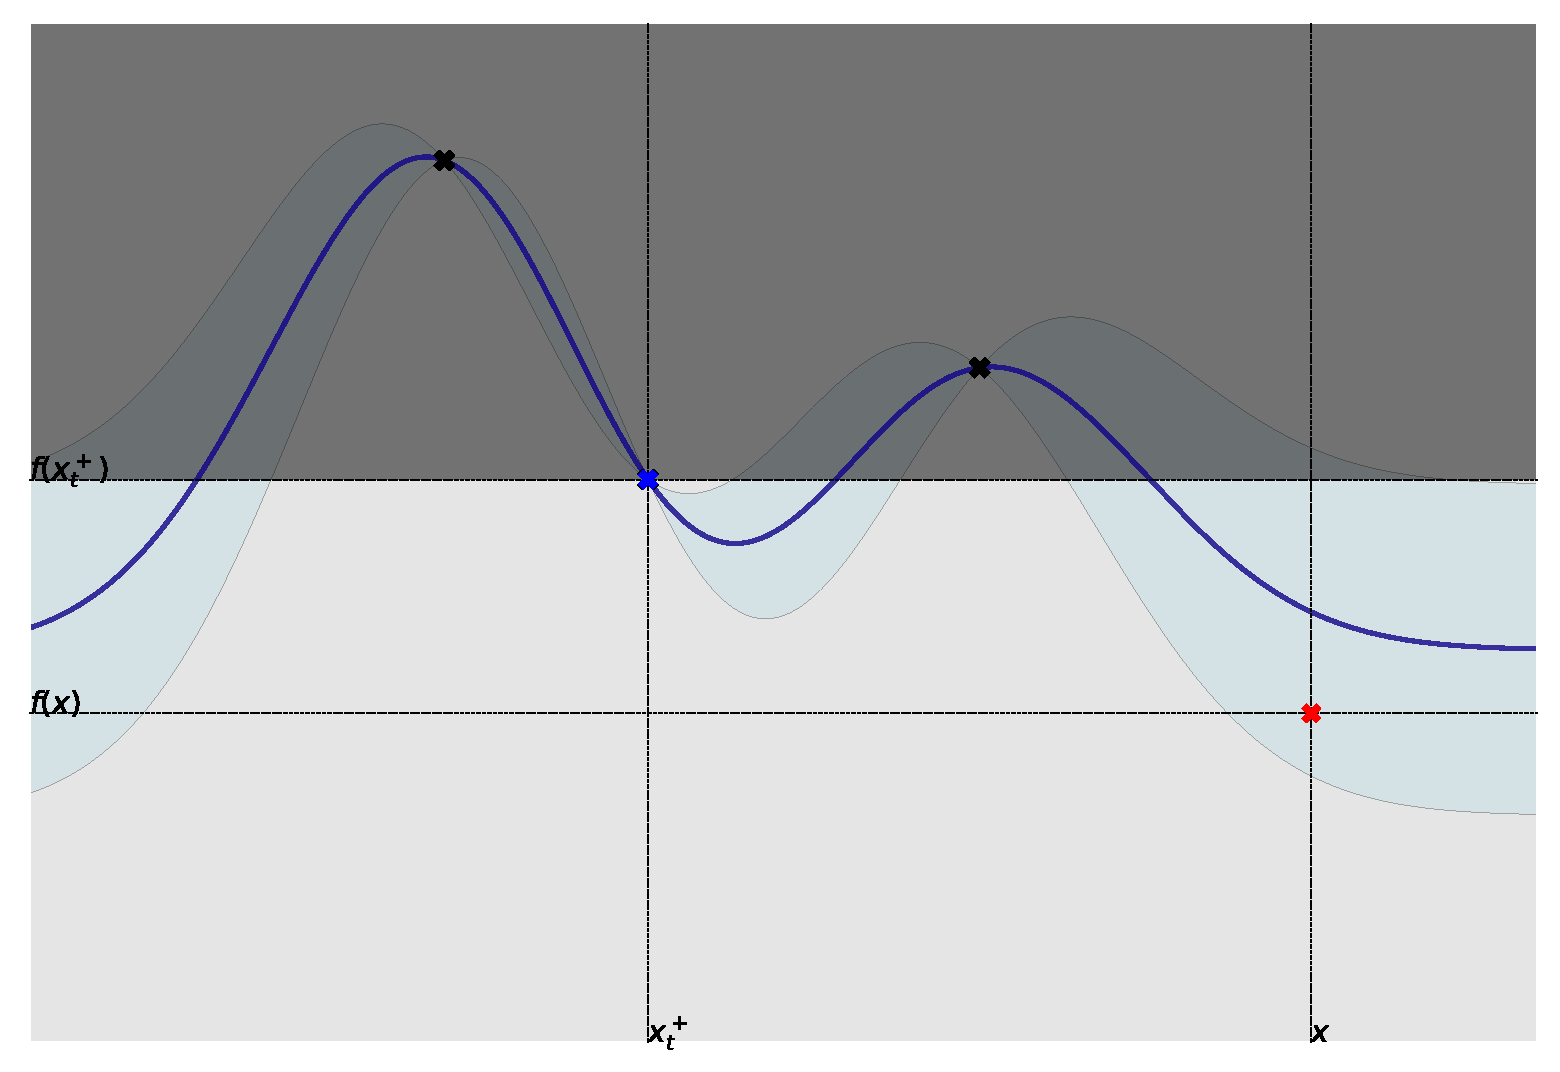
\includegraphics[width=.7\linewidth, height=0.7\textheight, keepaspectratio=true]{w06_hpo_bo/images/acq_func_images/ei_4.pdf}};
    \node<.> [below=0.01\belowcaptionskip of img4, align=center]{Hypothetical \emph{real} cost at a given $\conf$ - unknown in practice};

    \node<+> (img5) {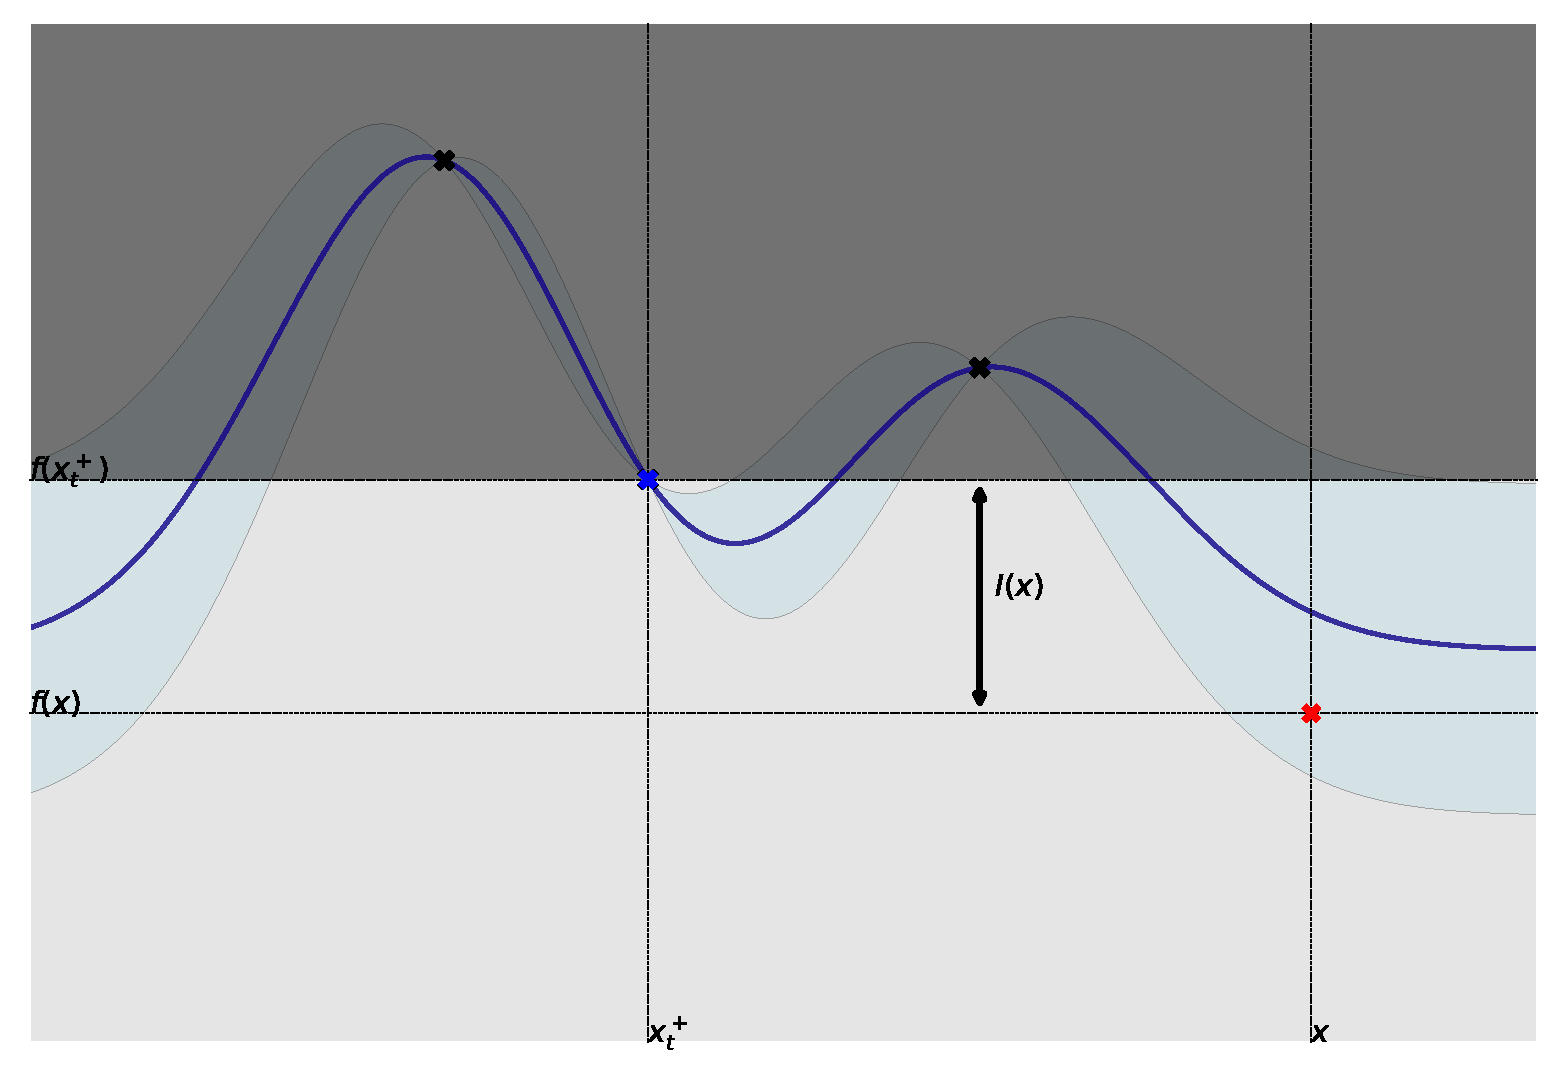
\includegraphics[width=.7\linewidth, height=0.7\textheight, keepaspectratio=true]{w06_hpo_bo/images/acq_func_images/ei_5.pdf}};
    \node<.> [below=0.01\belowcaptionskip of img4, align=center]{Actual improvement $I(\conf)$ - cannot be calculated before an evaluation!};

    \node<+> (img6) {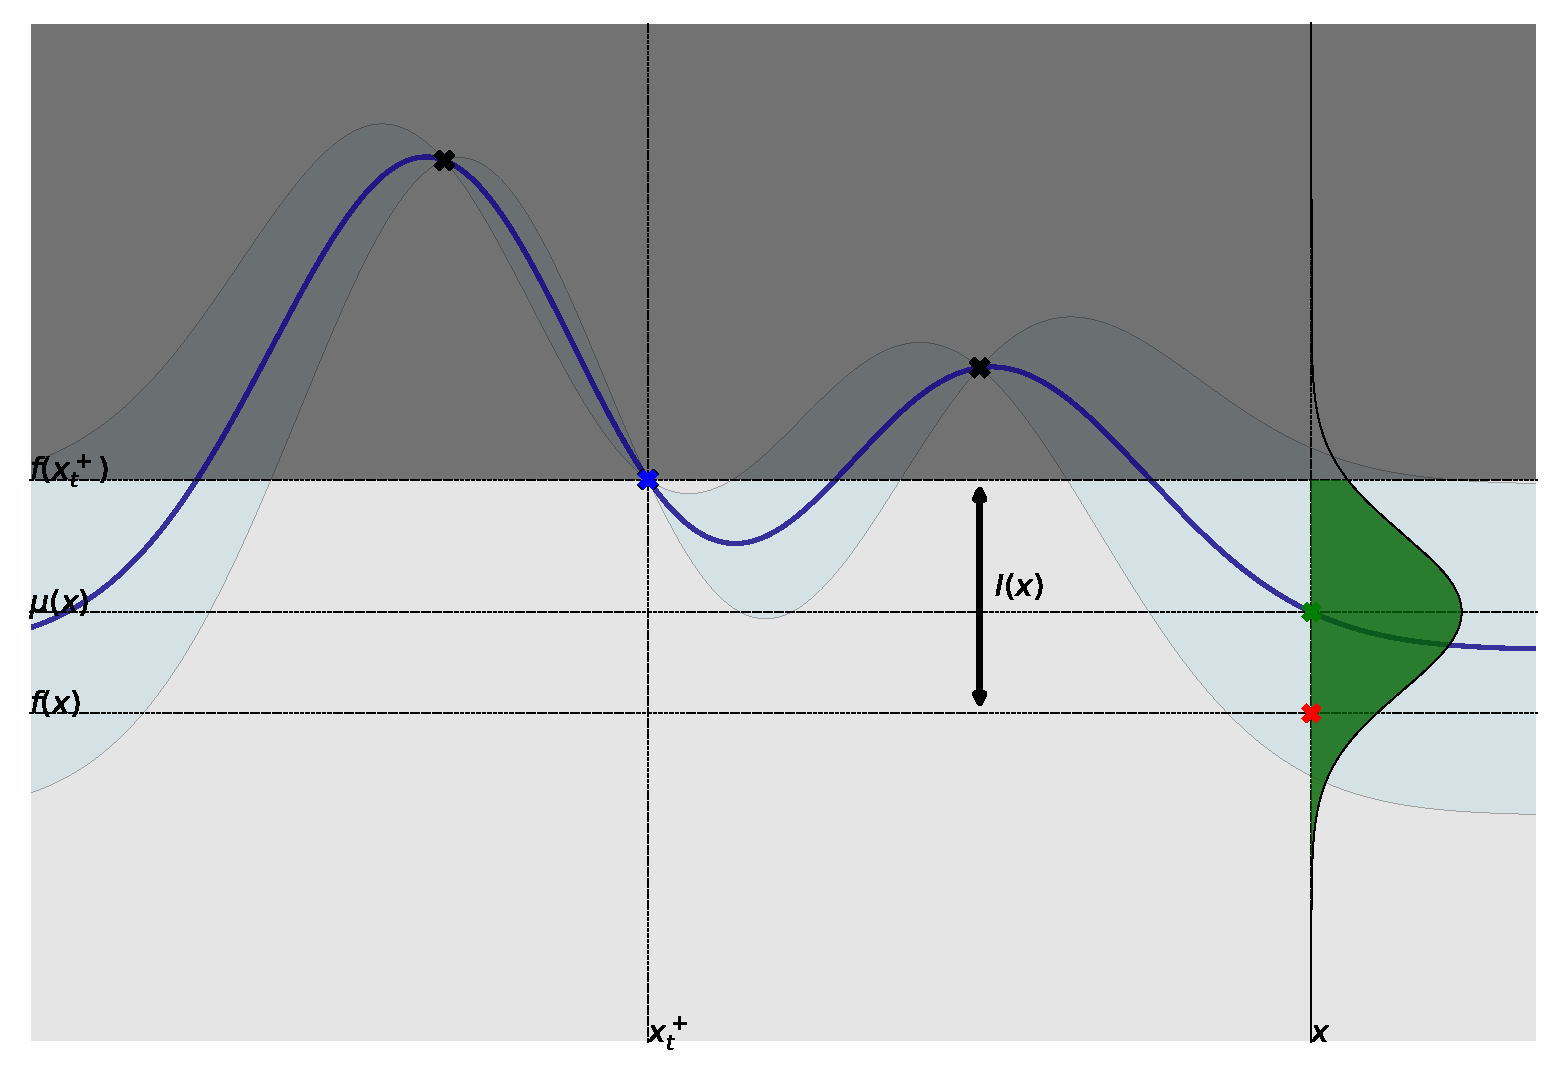
\includegraphics[width=.7\linewidth, height=0.7\textheight, keepaspectratio=true]{w06_hpo_bo/images/acq_func_images/ei_6.pdf}};
    \node<.> [below=-0.01\belowcaptionskip of img6, align=center]{$\E[\iter{\surro}(\conf)]$ - \emph{can} be calculated before an evaluation.};
    % \node<.> [below=-0.01\belowcaptionskip of img6, align=center]{$\E[\normaldist(\iter[\bocount-1]{\mean}(\conf), \iter[\bocount-1]{\left(\variance\right)}(\conf))]$ - \emph{can} be calculated before an evaluation.};

    \node<+> (img7) {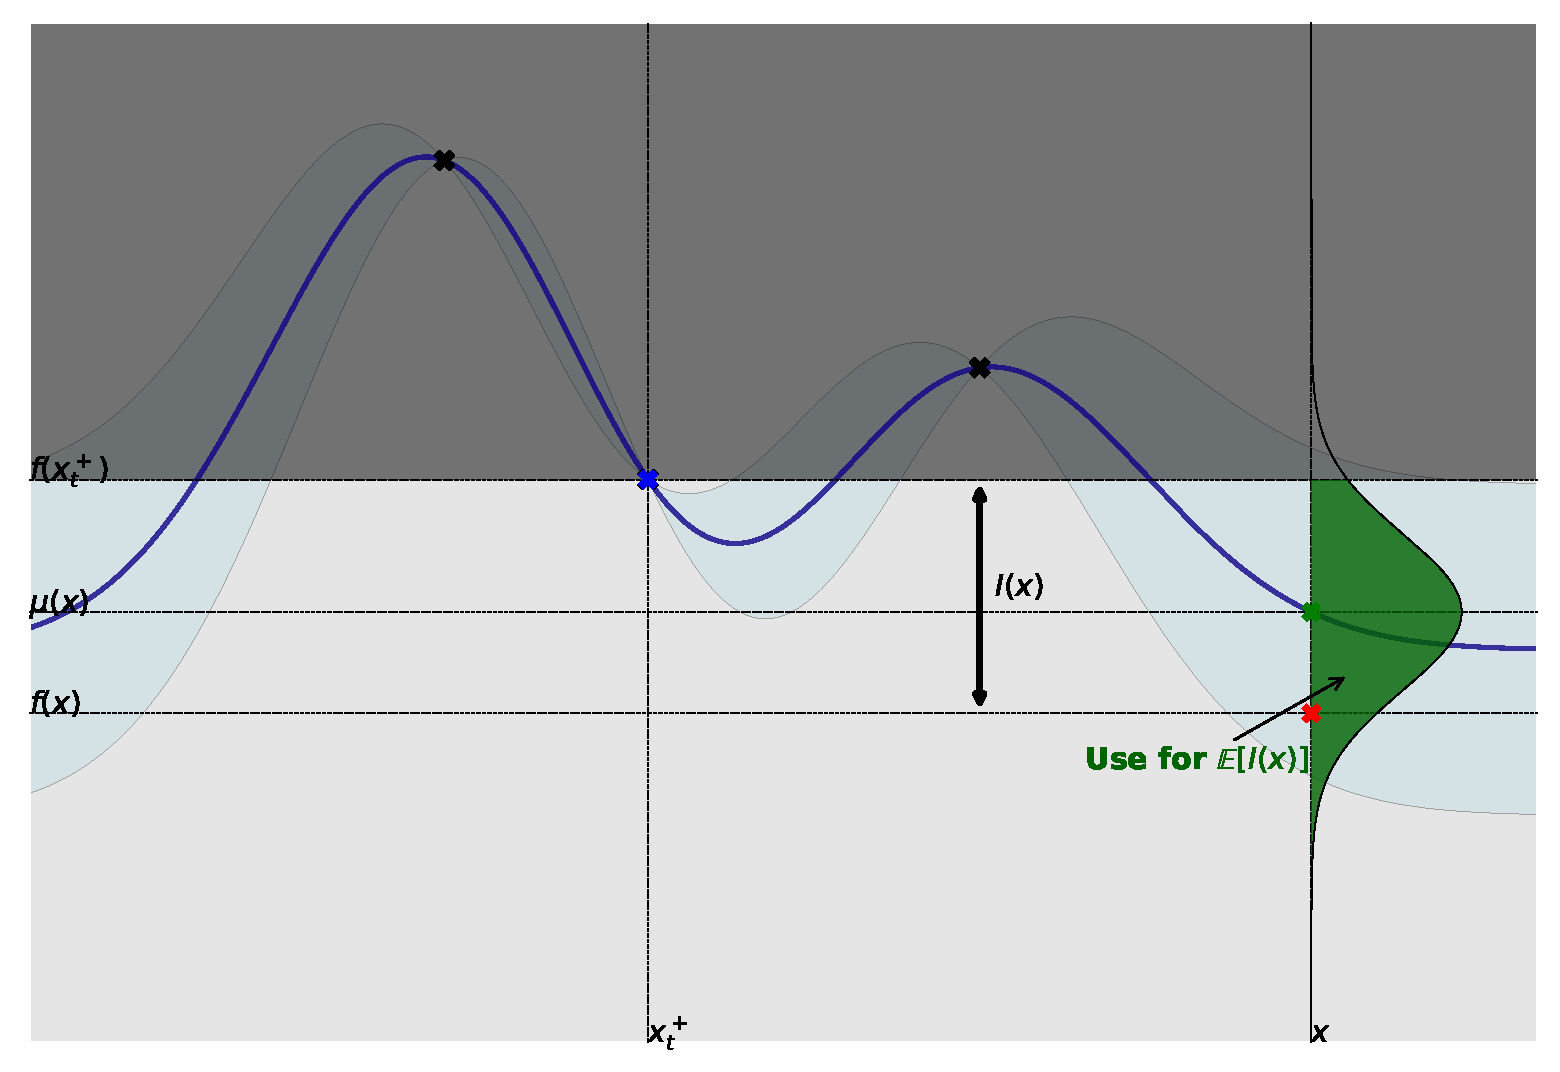
\includegraphics[width=.7\linewidth, height=0.7\textheight, keepaspectratio=true]{w06_hpo_bo/images/acq_func_images/ei_7.pdf}};
    \node<.> [below=0.01\belowcaptionskip of img7, align=center]{Use $\mean(\conf)$ and $\variance(\conf)$ to get $\E[I(\conf)]$};
  \end{tikzpicture}
\end{figure}

\end{frame}
%-----------------------------------------------------------------------
\begin{frame}[c]{Basic Acquisition Functions - EI}
\framesubtitle{Expected Improvement - Choosing a candidate}
\comment{Verify if formulae agree with minimizing the surrogate.}
\pause
\begin{itemize}\abovedisplayskip=0pt\belowdisplayskip=-0.5em
    \action<+->{\item[] We first define one-step improvement over the current incumbent, as}
    \action<+->{\[
        \iter{I}(\conf) = \max(0, \cost(\incumbent[\bocount-1]) - \cost(\conf)), \quad\incumbent[\bocount-1]\in\argmax_{\conf'\in\iter[\bocount-1]{\dataset}}\boobs\in\iter[\bocount-1]{\dataset}
    \]}
    \action<+->{\item[] Expected Improvement is then defined as}
    \begin{align*}
        \action<+->{\iter{EI}(\conf) &= \E[\iter{I}(\conf)]\\}
        \action<+->{&= \int_{\iter{I}=0}^{\iter{I}=\infty}\iter{I} P(\iter{I})d\iter{I}}
    \end{align*}
    \action<+->{\item[]If we use a normal distribution as the prior probability for $\iter{I}$,}
    \[
        \action<+->{P(\iter{I}) =
            \dfrac{1}{\sqrt{2\pi}\iter{\stddev}(\conf)}\exp{-\dfrac{{(\cost(\incumbent[\bocount-1])-\iter{\mean}(\conf)-\iter{I})}^2}{2\iter{\left(\variance\right)}(\conf)}}
        }
    \]
\end{itemize}
\end{frame}
%-----------------------------------------------------------------------
% \begin{frame}[c]{Basic Acquisition Functions - EI}
% \framesubtitle{Expected Improvement - Choosing a candidate}
%     \begin{align*}
%         \action<+->{\iter{EI}(\conf) &= \int_{\iter{I}=0}^{\iter{I}=\infty}\iter{I} \dfrac{1}{\sqrt{2\pi}\iter{\stddev}(\conf)}\exp{-\dfrac{{(\cost(\incumbent[\bocount-1])-\iter{\mean}(\conf)-\iter{I})}^2}{2\iter{\left(\variance\right)}(\conf)}}d\iter{I}\\}
%         \action<+->{&= 
%             \begin{cases}
%                 (\cost(\incumbent) - \iter{\mean}(\conf) - \xi)\cdf(Z) + \iter{\stddev}(\conf) \pdf(Z), & \text{if }\iter{\stddev}(\conf) > 0 \\
%                 0 & \text{if }\iter{\stddev}(\conf) = 0
%             \end{cases}\\}
%         \action<+->{\intertext{where }Z} \action<.->{&=\dfrac{\cost(\incumbent) - \iter{\mean}(\conf) - \xi}{\iter{\stddev}(\conf)}}
%     \action<+->{\Aboxed{\bonextsample \in \argmax_{\conf\in\pcs}(\iter{EI}(\conf))}}
%     \end{align*}
% %    \comment{Source: Tutorial by Brochu et al.: https://arxiv.org/pdf/1012.2599.pdf }
% \end{frame}
%-----------------------------------------------------------------------
\begin{frame}[c]{Basic Acquisition Functions - EI}
\framesubtitle{Expected Improvement - Choosing a candidate}
%     \comment{Consider this alternative formulation of EI for the previous slide.}
    \begin{align*}
        \action<+->{\iter{EI}(\conf) &= \int_{\iter{I}=0}^{\iter{I}=\infty}\iter{I} \dfrac{1}{\sqrt{2\pi}\iter{\stddev}(\conf)}\exp{-\dfrac{{(\cost(\incumbent[\bocount-1])-\iter{\mean}(\conf)-\iter{I})}^2}{2\iter{\left(\variance\right)}(\conf)}}d\iter{I}\\}
        \action<+->{&= 
            \begin{cases}
                \iter{\stddev}(\conf)[Z\cdf(Z) + \pdf(Z)], & \text{if }\iter{\stddev}(\conf) > 0 \\
                0 & \text{if }\iter{\stddev}(\conf) = 0
            \end{cases}\\}
        \action<+->{\intertext{where }Z} \action<.->{&=\dfrac{\cost(\incumbent[\bocount-1]) - \iter{\mean}(\conf) - \xi}{\iter{\stddev}(\conf)}}
    \action<+->{\Aboxed{\bonextsample \in \argmax_{\conf\in\pcs}(\iter{EI}(\conf))}}
    \end{align*}
%    \comment{Source: Tutorial by Brochu et al.: https://arxiv.org/pdf/1012.2599.pdf }
\end{frame}
%-----------------------------------------------------------------------
% \begin{frame}[c]{Basic Acquisition Functions - EI}
% \framesubtitle{Expected Improvement - Features}
% \comment{Replace with table of comparisons}
% \begin{itemize}
%     \item Enables an exploration-exploitation trade-off.
%     \item Analytical solutions for the multi-step setting exist.
%     \item One of the most commonly used acquisition functions.
% \end{itemize}
% \end{frame}
%-----------------------------------------------------------------------
\begin{frame}[c]{Basic Acquisition Functions - LCB/UCB}
\framesubtitle{Confidence Bounds - Concept}

\begin{figure}
  \centering
  \begin{tikzpicture}
    \node<+> (img1) {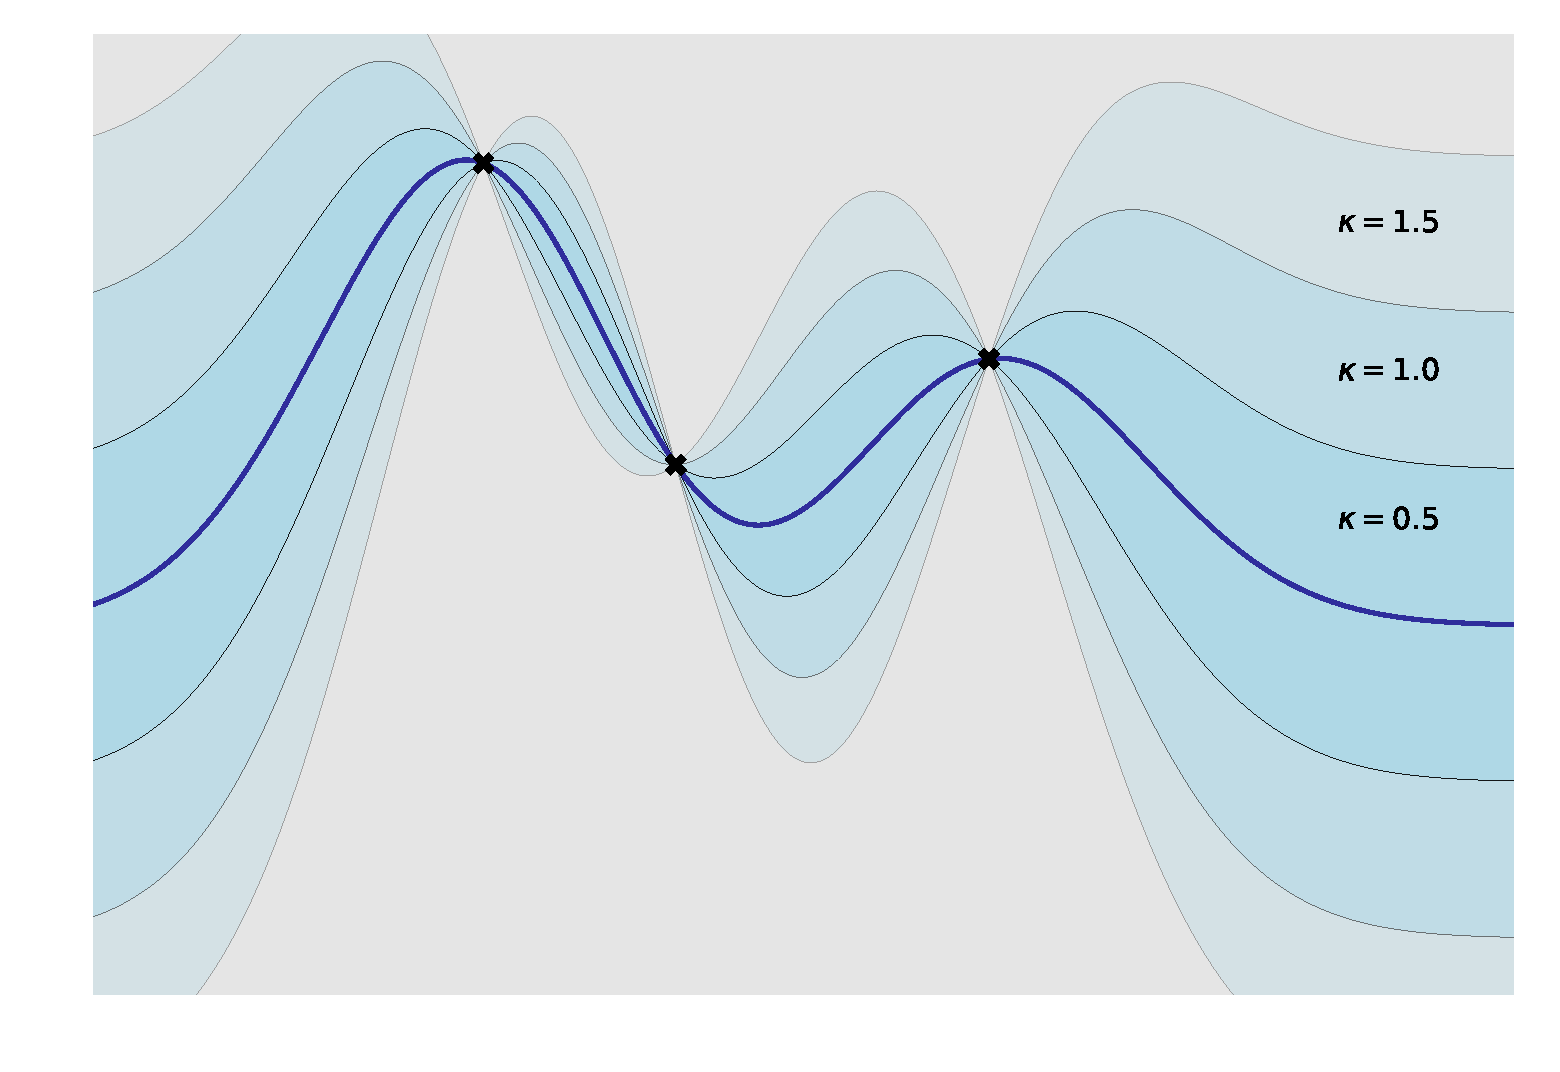
\includegraphics[width=.7\linewidth, height=0.7\textheight, keepaspectratio=true]{w06_hpo_bo/images/acq_func_images/lcb_1.pdf}};
    \node<.> [below=0.01\belowcaptionskip of img1, align=center]{Confidence Bound, $\mean(\conf)\pm\alpha\stddev(\conf)$};
    \node<+> (img2) {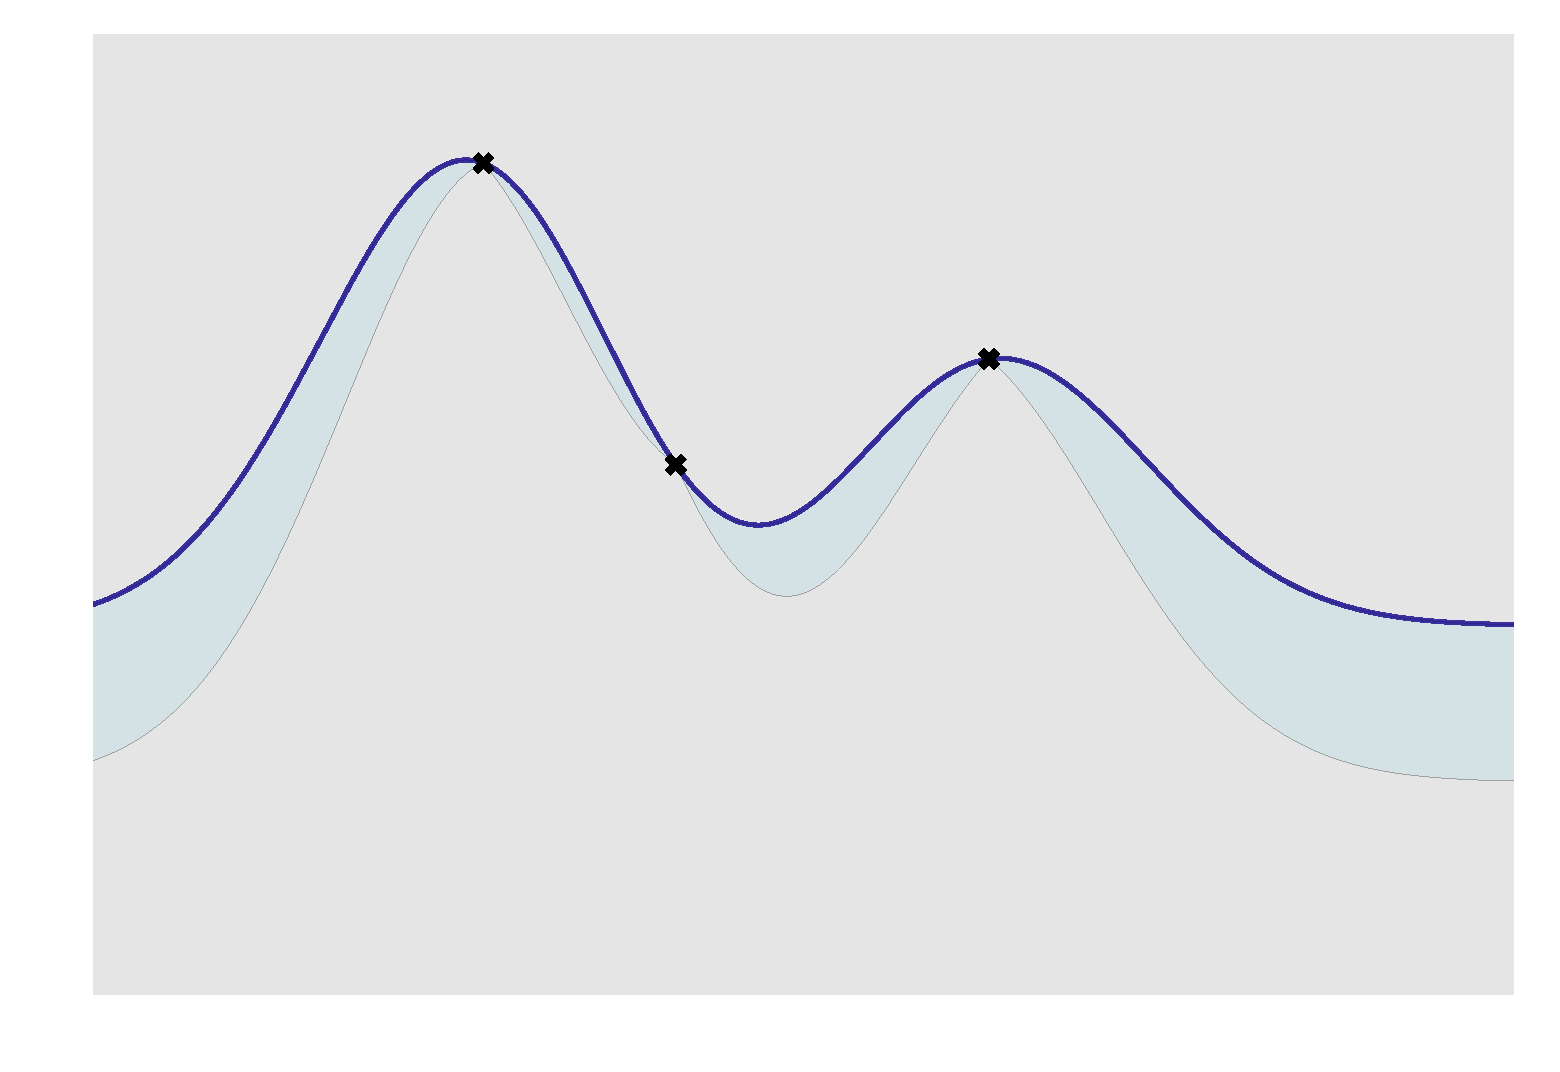
\includegraphics[width=.7\linewidth, height=0.7\textheight, keepaspectratio=true]{w06_hpo_bo/images/acq_func_images/lcb_2.pdf}};
    \node<.> [below=0.01\belowcaptionskip of img2, align=center]{Lower Confidence Bound, $\mean(\conf)-\alpha\stddev(\conf)$.};
    \node<+> (img3) {\includegraphics[width=.7\linewidth, height=0.7\textheight, keepaspectratio=true]{w06_hpo_bo/images/acq_func_images/lcb_3.pdf}};
    \node<.> [below=0.01\belowcaptionskip of img3, align=center]{To minimize cumulative regret, $\bonextsample=\argmin(LCB(\conf))$\comment{Verify!}};
  \end{tikzpicture}
\end{figure}

\end{frame}
%-----------------------------------------------------------------------
\begin{frame}[c]{Basic Acquisition Functions - LCB/UCB}
\framesubtitle{Confidence Bounds - Choosing a candidate}
\pause
\begin{itemize}
    \item<+->{We define the Lower Confidence Bound as 
    \[\iter{LCB}(\conf) = \iter{\mean}(\conf) - \alpha\iter{\stddev}(\conf),\quad\alpha\geq0\]}
    \item<+->{In the case of GPs, we define GP-LCB as
    \[\iter{GP-LCB}(\conf) = \iter{\mean}(\conf) - \sqrt{\nu\tau_t}\iter{\stddev}(\conf), \quad\nu>0\]}
    \item<+->{LCB is used to minimize cumulative regret.} 
    \item<+->{Question: When would you use Upper Confidence Bound (UCB) instead?}
    \comment{Source: Tutorial by Brochu et al.: https://arxiv.org/pdf/1012.2599.pdf }
\end{itemize}
\end{frame}
%-----------------------------------------------------------------------
% \begin{frame}[c]{Basic Acquisition Functions - LCB/UCB}
% \framesubtitle{Confidence Bounds - Features}
% \comment{Replace with table of comparisons}
% \begin{itemize}
%     \item Conceptually simple and easy to understand.
%     \item Inherently minimizes cumulative regret, or maximizes total reward.
%     \item Known theoretical guarantees under certain conditions for convergence.
%     \item Heavily dependent on the optimization of its hyperparameters - $\kappa$ in the general case, and $\nu$ and $\tau$ for the GP case.
% \end{itemize}
% \end{frame}
%-----------------------------------------------------------------------
\begin{frame}[c]{Basic Acquisition Functions - TS}
\framesubtitle{Thompson Sampling - Concept}

\begin{figure}
  \centering
  \begin{tikzpicture}
    \node<+> (img1) {\includegraphics[width=.7\linewidth, height=0.7\textheight, keepaspectratio=true]{w06_hpo_bo/images/acq_func_images/ts_1.pdf}};
    \node<.> [below=0.01\belowcaptionskip of img1, align=center]{Given the GP at iteration $\bocount$.};
    \node<+> (img2) {\includegraphics[width=.7\linewidth, height=0.7\textheight, keepaspectratio=true]{w06_hpo_bo/images/acq_func_images/ts_2.pdf}};
    \node<.> [below=0.01\belowcaptionskip of img2, align=center]{Draw a sample $g$ from the GP.};
    \node<+> (img3) {\includegraphics[width=.7\linewidth, height=0.7\textheight, keepaspectratio=true]{w06_hpo_bo/images/acq_func_images/ts_3.pdf}};
    \node<.> [below=0.01\belowcaptionskip of img3, align=center]{Now choose the minima of this sample.};
  \end{tikzpicture}
\end{figure}

\end{frame}
%-----------------------------------------------------------------------
\begin{frame}[c]{Basic Acquisition Functions - TS}
\framesubtitle{Thompson Sampling - Choosing a candidate}
\pause
\begin{itemize}
    \item Draw a sample $g$ from the GP $\iter{\gp}$.
    \pause
    \item Choose $\bonextsample=\argmin_{\conf\in\pcs}(g(\conf))$
\end{itemize}
\end{frame}
%-----------------------------------------------------------------------
\begin{frame}[c]{Basic Acquisition Functions - TS}
\framesubtitle{Thompson Sampling - Choosing a candidate}
\begin{center}
\begin{minipage}{0.75\textwidth}
\comment{Fix algorithm numbering}
\begin{algorithm}[H]
    %\DontPrintSemicolon
    \LinesNumbered
    \SetAlgoLined
    \setcounter{AlgoLine}{0}
    \SetKwInOut{Require}{Require}
    \SetKwInOut{Result}{Result}
    
    \Require{Initial dataset $\iter[0]{\dataset}$, budget $\bobudget$}
    \Result{$\iter[\bobudget]{\dataset}$ and $\finconf$}
    
    $\iter[0]{\dataset}\leftarrow\varnothing$,$\quad\gp(\cdot \given \iter[0]{\dataset})\leftarrow\gp(0, \kernel)$\;
    
    \For{$\bocount=1$ \KwTo $\bobudget$}{
    
        Fit $\iter{\gp}=\gp(\cdot \given \iter[\bocount-1]{\dataset})$\;
    
        Sample $g\sim\iter{\gp}$\;
    
        $\bonextsample\leftarrow\argmax_{\conf\in\pcs}g(\conf)$\;
    
        $\bonextobs\leftarrow \text{ Query }\cost\text{ at }\bonextsample$\;
    
        $\iter{\dataset}\leftarrow\iter[\bocount-1]{\dataset}\cup\{\langle\bonextsample,\bonextobs\rangle\}$\;}
    \caption{Thompson Sampling on a GP}
\end{algorithm}
\end{minipage}
\end{center}
%\comment{Source: Paper, Kandasamy et al, http://proceedings.mlr.press/v84/kandasamy18a/kandasamy18a.pdf}
\end{frame}
%-----------------------------------------------------------------------
% \begin{frame}[c]{Basic Acquisition Functions - TS}
% \framesubtitle{Thompson Sampling - Features}
% \comment{Replace with table of comparisons}
% \begin{itemize}
%     \item Not an acquisition function, but an acquisition \textit{method} instead.
%     \item Well-known theoretical bounds on maximum and minimum regret.
%     \item Simple Bayesian approach to solving the multi-armed bandit problem.
% \end{itemize}
% \end{frame}
    %-----------------------------------------------------------------------
\subsection{Advanced Acquisition Functions}
\begin{frame}[c]{Advanced Acquisition Functions}
\framesubtitle{Contents}
\pause
\begin{itemize}
    \item Concept: One-step look-ahead.
    \item Knowledge Gradient
    \item Entropy Search
    \item \emph{Maybe mention that we are now going to actually trust our surrogate to somewhat accurately model the underlying objective function (or that we are now risk-neutral) - thus relaxing one of the constraints mentioned in the very beginning of the section on Acquisition Functions.}
\end{itemize}
\end{frame}

%-----------------------------------------------------------------------

\begin{frame}[c]{Advanced Acquisition Functions}
%\framesubtitle{Knowledge Gradient - Concept}
\framesubtitle{One-Step Look Ahead}
\pause

\begin{figure}
  \centering
  \begin{tikzpicture}
    \node<+> (img1) {\includegraphics[width=.7\linewidth, height=0.7\textheight, keepaspectratio=true]{latex_main/images/placeholder.png}};
    \node<.> [below=0.01\belowcaptionskip of img1, align=center]{Once more, assume such a surrogate function GP $\iter{\gp}(\cdot)$ at time-step $\bocount$.};
    
    \node<+> (img2) {\includegraphics[width=.7\linewidth, height=0.7\textheight, keepaspectratio=true]{latex_main/images/placeholder.png}};
    \node<.> [below=0.01\belowcaptionskip of img2, align=center]{\emph{If} we evaluate $\cost(\cdot)$ at a random configuration $\conf$, $\iter[\bocount+1]{\gp}(\cdot\given {\conf})$ \emph{might} look like this. \\ \emph{Show what GP might look like at time-step $\bocount+1$.}};
    
    \node<+> (img3) {\includegraphics[width=.7\linewidth, height=0.7\textheight, keepaspectratio=true]{latex_main/images/placeholder.png}};
    \node<.> [below=0.01\belowcaptionskip of img3, align=center]{Mean - $\iter[\bocount+1]{\mean} \given_{\conf}$, Variance - $\iter[\bocount+1]{\left(\variance\right)} \given_{\conf}$, Minimum of the mean function - $\iter[\bocount+1]{\left(\mean^*\right)} \given_{\conf}$. \\\emph{Point out that all these quantities are now conditionally dependent on our choice of $\conf$}};
    
    \node<+> (img4) {\includegraphics[width=.7\linewidth, height=0.6\textheight, keepaspectratio=true]{latex_main/images/placeholder.png}};
    \node<.> [below=0.01\belowcaptionskip of img4, align=center]{This distribution is purely hypothetical - as shown by the conditional - \\and is called a one-step look-ahead. \emph{Just a re-statement of the GP's conditional nature at $\bocount+1$}};
  \end{tikzpicture}
\end{figure}

\end{frame}
%-----------------------------------------------------------------------

\begin{frame}[c]{Advanced Acquisition Functions - KG}
%\framesubtitle{Knowledge Gradient - Concept}
\framesubtitle{Knowledge Gradient - Concept}
\pause

\begin{figure}
  \centering
  \begin{tikzpicture}
    \node<+> (img1) {\includegraphics[width=.7\linewidth, height=0.7\textheight, keepaspectratio=true]{latex_main/images/placeholder.png}};
    \node<.> [below=0.01\belowcaptionskip of img1, align=center]{Once more, assume such a surrogate function GP $\iter{\gp}(\cdot)$ at time-step $\bocount$.};
    
    \node<+> (img2) {\includegraphics[width=.7\linewidth, height=0.6\textheight, keepaspectratio=true]{latex_main/images/placeholder.png}};
    \node<.> [below=0.01\belowcaptionskip of img2, align=center]{Given that we are risk-neutral, the configuration corresponding to the minimum \\of the mean function, $\iter{\left(\mean^*\right)}$, is the best choice here.};
    
    \node<+> (img3) {\includegraphics[width=.7\linewidth, height=0.7\textheight, keepaspectratio=true]{latex_main/images/placeholder.png}};
    \node<.> [below=0.01\belowcaptionskip of img3, align=center]{We perform a one-step look-ahead to get $\iter[\bocount+1]{\gp}(\cdot\given {\conf})$.};
    
    \node<+> (img4) {\includegraphics[width=.7\linewidth, height=0.7\textheight, keepaspectratio=true]{latex_main/images/placeholder.png}};
    \node<.> [below=0.01\belowcaptionskip of img4, align=center]{The best risk-neutral choice is again given by the minimum \\of the new conditional mean function - $\iter[\bocount+1]{\left(\mean^*\right)} \given_{\conf}$.};
    
    \node<+> (img5) {\includegraphics[width=.7\linewidth, height=0.7\textheight, keepaspectratio=true]{latex_main/images/placeholder.png}};
    \node<.> [below=0.01\belowcaptionskip of img5, align=center]{The expected value of the improvement in cost - from $\iter{\left(\mean^*\right)}$ to $\iter[\bocount+1]{\left(\mean^*\right)}$ - is \\ Knowledge Gradient. \emph{Show side-by-side comparison of the two GPs}};
  \end{tikzpicture}
\end{figure}

\end{frame}
%-----------------------------------------------------------------------
\begin{frame}[c]{Advanced Acquisition Functions - KG}
\framesubtitle{Knowledge Gradient - Choosing a candidate}
\pause
\begin{itemize}\abovedisplayskip=0.5em\belowdisplayskip=0.5em
    \action<+->{\item Given a GP $\iter{\gp}$ fit on $\iter[\bocount-1]{\dataset}$, on the $\bocount\,$th iteration we have}
    \action<+->{\[\iter{\left(\mean^*\right)} = \max_{\conf'\in\pcs}(\iter{\mean}(\conf'\given{\dataset_{\bocount-1}}))\]}
    \action<+->{\item If we choose a candidate $\bonextsample=\conf$ to evaluate $\cost(\cdot)$ at,}
    %\action<+->{\[\dataset_{\bocount}\given{\conf} = \{(\conf_1, \boobs_1),\dots,(\conf_{\bocount-1}, \boobs_{\bocount-1})\}\cup\{(\iter{\conf},\iter{\boobs})\given{\bonextsample=\conf}\}.\]}
    \action<+->{\[\iter{\dataset}\given\conf = \iter[\bocount-1]{\dataset}\cup\{\langle\bonextsample,\,\bonextobs\rangle\given{\bonextsample=\conf}\}.\]}
    \action<+->{\item Thus, if we hypothesize about the $\bocount+1\,$th iteration, we would get}
    \action<+->{\[\iter[\bocount+1]{\left(\mean^*\right)} \given_{\conf} = \max_{\conf'\in\pcs}(\iter[\bocount+1]{\mean}(\conf'\given{\iter{\dataset},\bonextsample=\conf}))\]}
\end{itemize}
\comment{Source:https://arxiv.org/pdf/1807.02811.pdf}
\end{frame}
%-----------------------------------------------------------------------
\begin{frame}[c]{Advanced Acquisition Functions - KG}
\framesubtitle{Knowledge Gradient - Choosing a candidate}
\begin{itemize}\abovedisplayskip=1em\belowdisplayskip=0em
    \action<+->{\item In a risk-neutral setting, $\iter{\left(\mean^*\right)}$ and $\iter[\bocount+1]{\left(\mean^*\right)}$ are the global optima for $\iter{\mean}$ and $\iter[\bocount+1]{\mean}\given_{\conf}$ respectively.}
    \action<+->{\item Thus, the conditional improvement in the cost (adjusted for maximization) is \[\iter{\left(\mean^*\right)} - \left.\iter[\bocount+1]{\left(\mean^*\right)} \right|_{\bonextsample=\conf}\]}
    \action<+->{\item We cannot directly compute this improvement, but we can compute its expected value, which we call Knowledge Gradient:}
    \action<+->{\[\iter{KG}(\conf) = \E\left[ \iter{\left(\mean^*\right)} - \left. \iter[\bocount+1]{\left(\mean^*\right)} \right|_{\bonextsample=\conf} \right]\]}
    \action<+->{\item Finally, \[\boxed{\bonextsample = \argmax_{\conf\in\pcs}(\iter{KG}(\conf))}\]}
\end{itemize}
\comment{Source:https://arxiv.org/pdf/1807.02811.pdf}
\end{frame}
%-----------------------------------------------------------------------
\begin{frame}[c]{Advanced Acquisition Functions - ES}
\framesubtitle{Entropy Search - Concept}
\pause

\begin{figure}
  \centering
  \begin{tikzpicture}
    \node<+> (img1) {\includegraphics[width=.7\linewidth, height=0.6\textheight, keepaspectratio=true]{latex_main/images/placeholder.png}};
    \node<.> [below=0.01\belowcaptionskip of img1, align=center]{We consider the global optimum's position to be a random variable $\conf^*$, \\with uniform prior probability. \emph{Show the probability distribution below the GP throughout ES}};
    
    \node<+> (img2) {\includegraphics[width=.7\linewidth, height=0.7\textheight, keepaspectratio=true]{latex_main/images/placeholder.png}};
    \node<.> [below=0.01\belowcaptionskip of img2, align=center]{The minimum of a sample from the GP $\iter{\gp}$ provides some evidence for where $\conf^*$ may lie. \\\emph{Visualization for demonstrative purposes only, not actual implementation.}};
    
    \node<+> (img3) {\includegraphics[width=.7\linewidth, height=0.7\textheight, keepaspectratio=true]{latex_main/images/placeholder.png}};
    \node<.> [below=0.01\belowcaptionskip of img3, align=center]{Each new sample provides more information about where the global minimum lies - \\i.e. has an assosciated \emph{information gain}.};
    
    \node<+> (img4) {\includegraphics[width=.7\linewidth, height=0.7\textheight, keepaspectratio=true]{latex_main/images/placeholder.png}};
    \node<.> [below=0.01\belowcaptionskip of img4, align=center]{After $S$ such samples, we can narrow down the approximate location of the global minimum\\ i.e. reduce entropy of the search space.};
  \end{tikzpicture}
\end{figure}

\end{frame}
%----------------------------------------------------------------------
\begin{frame}[c]{Advanced Acquisition Functions - ES}
\framesubtitle{Entropy Search - Choosing a candidate}
\begin{itemize}
    \item Provide formulae for entropy search - pseudocode for the sampling-based version, formula for overall entropy search (integral of H) only
    \item Mention existence of more complicated but efficient search procedure, mention differences.
    \item Mention: Repeated Thompson Sampling is an approximation to sampling based entropy-search.
    \item Provide link to paper.
\end{itemize}
\comment{Source:https://arxiv.org/pdf/1807.02811.pdf}
\end{frame}
%-----------------------------------------------------------------------
    \videotitle{Surrogate Models}

%-----------------------------------------------------------------------
\myframetop{Desiderata for Surrogate Models in Bayesian Optimization}{

    \begin{columns}[T] % align columns
    \begin{column}{.48\textwidth}
    \only<1-2>{
        \begin{block}{In all cases}
        \begin{itemize}
        	\item Regression model with uncertainty estimates
        	\item Accurate predictions
        \end{itemize}
        \end{block}
    }
    \only<2-2>{
        \begin{block}{Depending on the application}
        \begin{itemize}
        	\item Is cheap to train
        	\item Scales well in the number of data points
        	\item Scales well in the number of dimensions
        	\item Can handle different types of inputs (categorical and continuous)
        \end{itemize}
        \end{block}
    }
    \end{column}%
    
    \hfill%
    
    \begin{column}{.48\textwidth}
    \bigskip
    \bigskip
    %\only<1-1>{\includegraphics[width=1.\textwidth]{images/bo_loop_overview/03_mean.png}}
    %\only<2-6>{
    \includegraphics[width=\textwidth]{images/bo_loop_overview/Uncertainty.pdf}
    %}
    
    \end{column}%
    \end{columns}
}
%-----------------------------------------------------------------------

%-----------------------------------------------------------------------
%-----------------------------------------------------------------------
\begin{frame}[c]{Overview of the Surrogate Models We'll Discuss}

%\begin{columns}[T] % align columns
%\begin{column}{.38\textwidth}
%\begin{minipage}[c][.6\textheight][c]{\linewidth}
\begin{itemize}
	\item Gaussian Processes \note[item]{(quite common)}
	\item Random Forests \note[item]{(our default choice)}
	\item Bayesian Neural Networks \note[item]{(recent trend)}

\end{itemize}
%\end{minipage}
%\end{column}%

%\hfill%
%\begin{column}{.58\textwidth}
%
%\begin{columns}[T] % align columns
%\begin{column}{.48\textwidth}
%    \includegraphics[width=1.\textwidth]{images/surrogate_models/uncertainty_gp.jpg}
%\end{column}%
%
%\hfill%
%
%\begin{column}{.48\textwidth}
%    \includegraphics[width=1.\textwidth]{images/surrogate_models/uncertainty_forest.jpg}
%\end{column}%
%\end{columns}
%
%\vspace*{\fill}
%\begin{center}
%  \includegraphics[width=.6\textwidth]{images/surrogate_models/uncertainty_dngo.jpg}
%  
%\end{center}
%\vspace*{\fill}
%
%\end{column}%
%\end{columns}
%
%\hspace{5.5cm}\footnotesize{Image source: \lit{\href{}{A. Klein: Introduction Automated Machine Learning}}}


\end{frame}
%-----------------------------------------------------------------------
\begin{frame}[c]{Gaussian Processes (GPs): Reminder of Pros and Cons}

\begin{columns}[T] % align columns
\begin{column}{.48\textwidth}

    \begin{block}{Advantages}
    \begin{itemize}
    	\item Smooth and reliable uncertainty estimates 
		\item Strong sample efficiency
    	\item We can encode expert knowledge about the design space in the kernel 
    \end{itemize}
    \end{block}
\bigskip
\fhpause
\hspace*{0.5cm}These advantages make GPs the\\
\hspace*{0.5cm}\alert{most commonly-used model\\
\hspace*{0.5cm}in Bayesian optimization}

\end{column}%

\hfill%
\fhpause

\begin{column}{.48\textwidth}
    \begin{block}{Disadvantages}
    \begin{itemize}
    	\item Performance can be quite sensitive to the choice of kernel
    	\note[item]{(if we don't optimize small-dimensional, continuous functions)}
    	\item Cost scales cubically with the number of observations 
    	\item Weak performance for high dimensionality
    	\note[item]{(because of inverting the kernel)}
    	\item Not easily applicable in discrete or conditional spaces 
    	\item Sensitive to its own hyperparameters
    \end{itemize}
\end{block}

\end{column}
\end{columns}

\note[item]{
	\begin{itemize}
		 \item e.g., special kernels for categorical hyperparameters and\\ conditional dependencies
	\end{itemize}
}
	
\note[item]{
    \begin{itemize}
    	\item to address this issue, there are sparse GPs\\ \lit{Snelson and Ghahramani. 2005}
    \end{itemize}
}

\end{frame}
%-----------------------------------------------------------------------

%-----------------------------------------------------------------------
%-----------------------------------------------------------------------
%\begin{frame}[c]{Gaussian Processes - reminder}
%
%\begin{itemize}
%    \item<1-3> The prior is a GP with constant mean and variance; draws are jointly Gaussian
%    \item<2-3> The kernel (covariance) function $K$ tells us how correlated the function values at two points are
%    \item<3-3> The posterior is also a GP, with predictive distribution:
 %   \begin{equation*}
 %        P(\func_{\bocount+1} \vert \dataset_{1:\bocount}, \conf_{\bocount+1}) =  \mathcal{N}(\mean_{\bocount}(\conf_{\bocount+1}), \variance_{\bocount}(\conf_{\bocount+1}))
 %   \end{equation*}
 %   \begin{equation*}
 %       \mean_{\bocount}(\conf_{\bocount+1}) = \bm{k}^{T} \bm{K}^{-1} \bm{\func_{1:\bocount}}
 %   \end{equation*}
 %   \begin{equation*}
 %       \variance_{\bocount}(\conf_{\bocount+1}) = k(\conf_{\bocount+1}, \conf_{\bocount+1}) - \bm{k}^{T} \bm{K}^{-1} \bm{k}
 %   \end{equation*}
%\end{itemize}
%
%\note[item]{for the review of GPs - Rasmussen and Williams}
%
%\end{frame}
%-----------------------------------------------------------------------
 
% %-----------------------------------------------------------------------
% %-----------------------------------------------------------------------
% \begin{frame}[c]{Surrogate Models: GPs - kernel hyperparameters}

% \begin{itemize}
%     \item After choosing the kernel, we must also manage the hyperparameters that govern its behaviour, as well as that of the mean function.  \fhpause
%     \item For our problems of interest, typically we have $D + 3$ GPs hyperparameters:  
%     \begin{itemize}
%         \item $D$ length scales $\theta_{1:D}$, 
%         \item the covariance amplitude $\theta_{0}$, 
%         \item the observation noise $\noise$, 
%         \item a constant mean $\mean$. 
%     \end{itemize}
% \end{itemize}

% \end{frame}
% %-----------------------------------------------------------------------


%-----------------------------------------------------------------------
%-----------------------------------------------------------------------
\begin{frame}[c]{Gaussian Processes (GPs): Kernel Hyperparameters}

\begin{columns}[T] % align columns
\begin{column}{.6\textwidth}
\begin{itemize}
    \item We could optimize GP hyperparameters (maximum likelihood, MLE, or maximum a posteriori, MAP)


    \item<+-> But \alert{sampling} GP  hyperparameters from the posterior distribution performs better; e.g., via \alert{Markov-Chain Monte-Carlo (MCMC)}


    \item<+-> \alert{Marginalize} over GP hyperparameters $\theta$ and compute an \alert{integrated acquisition function}:
        \begin{equation*}
        \begin{aligned}
            \Bar{\acq}(\conf) = \int \acq (\conf, \surro_\theta)p(\theta)d\theta
        \end{aligned}
        \end{equation*}

 
    \item<+-> Downside: computational expense
    \myit{
        \item MCMC is computationally expensive
        \item Acquisition function now has to be calculated for each sample
    }
\end{itemize}
\end{column}
%
\begin{column}{.4\textwidth}
\only<2->{
    \centering
    \includegraphics[width=0.7\textwidth]{images/surrogate_models/kernel_hp_mcmc.jpg}
    
    \footnotesize{Image source: \lit{\href{https://arxiv.org/pdf/1206.2944.pdf}{Snoek et al. 2012}}}
}


   
\end{column}

\end{columns}

\end{frame}
%-----------------------------------------------------------------------
\begin{frame}[c]{Random Forests (RFs): Reminder \& How To Compute Uncertainties}

\centering
    \includegraphics[width=0.5\textwidth]{images/surrogate_models/random_forest_pic}

\begin{columns}[T] % align columns
\begin{column}{.48\textwidth}

\begin{block}{RF Training}
\begin{itemize}
	\item Fit a set of \alert{randomized} regression trees
	\item Randomization via bootstrapping \& random selection of split variables / split points
	\item Each tree yields a possible explanation for the observations
\end{itemize}
\end{block}
\end{column}

\fhpause
\hfill

\begin{column}{.48\textwidth}
    \begin{block}{RF Prediction}
    \begin{itemize}
    	\item Predict with each tree
    	\item Aggregate predictions (e.g., average)
    	\item Uncertainty estimate:\\ \alert{empirical variance across tree predictions}
    \end{itemize}
    \end{block}
\end{column}
\end{columns}

\end{frame}
%-----------------------------------------------------------------------
\begin{frame}[c]{Random Forests (RFs): Impact of Basic Model Choices}
\vspace{-25pt}

\begin{columns}
\column{0.5\textwidth}

\begin{figure}[h]
\captionsetup[subfigure]{position=top}
\centering

\renewcommand{\thesubfigure}{a}
\subfloat[][no bootstrapping, \\ no random splits]{
\includegraphics[width=0.55\textwidth, clip]{images/surrogate_models/rf_noboot_middle_split.png}

}
\qquad
\renewcommand{\thesubfigure}{b}
\subfloat[][with bootstrapping, \\ no random splits]{
\includegraphics[width=0.55\textwidth, clip]{images/surrogate_models/rf_boot_middle_split.png}
}
\end{figure}

\column{0.5\textwidth}
\begin{figure}[h]
\captionsetup[subfigure]{position=top}
\centering

\fhpause
\renewcommand{\thesubfigure}{c}
\subfloat[][no bootstrapping, \\ with random splits]{
\includegraphics[width=0.55\textwidth, clip]{images/surrogate_models/rf_noboot_rand_split.png}

}
\qquad
\renewcommand{\thesubfigure}{d}
\subfloat[][with bootstrapping, \\ with random splits]{
\includegraphics[width=0.55\textwidth, clip]{images/surrogate_models/rf_boot_rand_split.png}
}

\end{figure}
\end{columns}

\end{frame}
%-----------------------------------------------------------------------
\begin{frame}[c]{Random Forests (RFs): Overview of Pros and Cons}

\begin{columns}[T] % align columns
\begin{column}{.48\textwidth}

    \begin{block}{Advantages}
    \begin{itemize}
        \item Cheap to train 
        \item Scales well with \#observations $n$: 
        \begin{itemize}
        	\item Fitting: $O(n \log n)$ 
        	\item Prediction: $O(\log n)$
        \end{itemize}
        \item Scales well with \#dimensions
        \item Training can be parallelized 
        \item Can easily handle conditional, categorical, continuous and discrete spaces 
        \item Quite robust against its own hyperparameters
    \end{itemize}
    \end{block}
\end{column}%

\hfill%
\fhpause

\begin{column}{.48\textwidth}
    \begin{block}{Disadvantages}
    \begin{itemize}
        \item Poor uncertainty estimates 
        \item Poor extrapolation (constant) 
    	\item Priors cannot be incorporated easily 
    \end{itemize}
    \end{block}

\fhpause
\bigskip
\bigskip
\hspace*{0.5cm}These qualities make RFs a \alert{robust} \\
\hspace*{0.5cm}\alert{option} for Bayesian optimization in \\ \hspace*{0.5cm}\alert{high dimensions}, for \alert{categorical spaces},\\
\hspace*{0.5cm}or when function evaluations are quite fast

\end{column}
\end{columns}

\end{frame}
%-----------------------------------------------------------------------
\begin{frame}[c]{Bayesian Neural Networks: Overview}

\begin{itemize}
    \item Neural networks are more flexible \& scalable than Gaussian processes 
    \item But for use in Bayesian optimization, neural networks need to be made probabilistic
    
\fhpause
    \item Bayesian deep learning aims to deal with all sources of uncertainty \fhpause
    \begin{itemize}
        \item E.g., we don't have a single weight vector anymore, but a distribution over weights
    \end{itemize}

\centering
\includegraphics[width=0.6\textwidth]{images/surrogate_models/bnn.jpg}

\footnotesize{Image source: \lit{\href{http://proceedings.mlr.press/v37/blundell15.pdf}{Blundell et al. 2015}}}

\end{itemize}



\end{frame}
%-----------------------------------------------------------------------
%\begin{frame}[c]{Surrogate Models: Bayesian Neural Networks - Idea}
%
%\begin{itemize}
%    \item Extend regression NNs to model uncertainty
%    \item Deal with all sources of parameter uncertainty
%    \item If possible, one would also deal with uncertainty about the network architecture
%     \begin{itemize}
%        \item For every architecture, one would still want to be Bayesian about its weights... 
%        \item Nobody is really Bayesian about architectures these days 
%        \item This has been too expensive; but that may change with efficient gradient-based architecture search methods...
%    \end{itemize}
%\end{itemize}
%
%\end{frame}

%-----------------------------------------------------------------------

\begin{frame}[c]{Simplest Way of Incorporating Uncertainty in Neural Networks: DNGO}


\begin{itemize}
    \item Fit a standard regression neural network to the data (with a linear output layer)
    \item Use the representation in the last hidden layer as \alert{basis functions $\phi(x)$} of the input $x$ 
    \item \alert{Use Bayesian linear regression with these basis functions} \fhpause
    \begin{itemize}
        \item The last layer is linear in its parameters $\theta$  
        \item Therefore, the Bayesian linear regression formulas work directly 
        \item Feasible in closed form, in time $O(N d^3)$, where $N$ is the number of data points\\ and $d$ is the number of hidden units in the last layer 
    \end{itemize}
    \item Not fully Bayesian yet, but already allows scalable Bayesian optimization \lit{\href{https://arxiv.org/pdf/1502.05700.pdf}{Snoek et al. 2015}}

\end{itemize}

%\vspace{1cm}
%\hspace{12cm}
%\lit{\href{https://arxiv.org/pdf/1502.05700.pdf}{Snoek et al. 2015}}

\end{frame}


%-----------------------------------------------------------------------

\begin{frame}[c]{Bayesian Optimization with BNNs: Overview of Existing Approaches}

\begin{itemize}
	    \item \lit{\href{https://arxiv.org/pdf/1502.05700.pdf}{Snoek et al. 2015}} Scalable Bayesian Optimization Using Deep Neural Networks (DNGO)
	    \item \lit{\href{https://papers.nips.cc/paper/6117-bayesian-optimization-with-robust-bayesian-neural-networks.pdf}{Springenberg et al. 2016}} Bayesian Optimization with Robust Bayesian Neural Networks
	    \item \lit{\href{https://arxiv.org/abs/1706.01825}{Hern\'andez-Lobato et al. 2017}} Parallel and Distributed Thompson Sampling for Large-scale Accelerated Exploration of Chemical Space
\bigskip
\fhpause
        \item \lit{\href{https://www.ismll.uni-hildesheim.de/pub/pdfs/schilling2015-ecml.pdf}{Schilling et al. 2015}} Hyperparameter Optimization with Factorized Multilayer Perceptrons
        \item \lit{\href{https://papers.nips.cc/paper/7917-scalable-hyperparameter-transfer-learning}{Perrone et al. 2018}} Scalable Hyperparameter Transfer Learning

\end{itemize}

\end{frame}
%-----------------------------------------------------------------------
\begin{frame}[c]{Bayesian Neural Networks (BNNs): Overview of Pros and Cons}

\begin{columns}[T] % align columns
\begin{column}{.48\textwidth}

    \begin{block}{Advantages}
    \begin{itemize}
        \item Scales linearly with \#observations 
        \item Can obtain nice and smooth uncertainty estimates 
        \item Flexibility: handling of categorical, continuous and discrete spaces
    \end{itemize}
    \end{block}

\onslide<3->{
\bigskip
\bigskip
\hspace*{0.5cm}These qualities make BNNs an \\
\hspace*{0.5cm}\alert{ever-more promising alternative}
%\hspace*{0.5cm}Needed: robust auto-tuned(?) implementation
}
\end{column}%

\hfill%

\begin{column}{.48\textwidth}
\onslide<2->{
    \begin{block}{Disadvantages}
    \begin{itemize}
    	\item Usually needs more data than Gaussian processes
    	\item Uncertainty estimates often worse than for Gaussian processes 
        \item Many meta-design decisions 
    	\item No robust off-the-shelf implementation 
    \end{itemize}
    \end{block}
}
\end{column}
\end{columns}

\end{frame}
%-----------------------------------------------------------------------
\begin{frame}[c]{Bayesian Neural Networks (BNNs): Further Reading}

There is a lot more work on BNNs that hasn't been applied to Bayesian optimization yet:
\begin{itemize}
%        \item \lit{\href{https://www.cs.utoronto.ca/~radford/bnn.book.html}{Neal 1995}} Bayesian Learning for Neural Networks
%        \item \lit{\href{https://www.microsoft.com/en-us/research/uploads/prod/2006/01/Bishop-Pattern-Recognition-and-Machine-Learning-2006.pdf}{Bishop 2006}} Pattern Recognition and Machine Learning
        \item Ensembles obtained simply by running SGD several times \lit{\href{https://arxiv.org/abs/1612.01474}{Lakshminarayanan et al. 2017}}
        %: Simple and Scalable Predictive Uncertainty Estimation using Deep Ensembles
        \item Dropout \lit{\href{https://arxiv.org/abs/1506.02142}{Gal et al. 2016}} 
        %Dropout as a Bayesian Approximation:
        %Representing Model Uncertainty in Deep Learning
        \item Monte Carlo Batch Normalization \lit{\href{https://arxiv.org/abs/1802.06455}{Teye et al. 2018}} %Bayesian Uncertainty Estimation for Batch Normalized Deep Networks
        \item Snapshot Ensembles \lit{\href{https://arxiv.org/abs/1704.00109}{Gao Huang et al. 2017}} 
        %Snapshot Ensembles: Train 1, get M for free
\end{itemize}


\end{frame}
%-----------------------------------------------------------------------
\begin{frame}[c]{Questions to Answer for Yourself / Discuss with Friends}

\begin{itemize}
    %GP
%    \item \alert{Repetition.} What are the most important hyperparameters of a GP that you would want to optimize for Bayesian Optimization? 
    %RF
    \item \alert{Discussion.} For which optimization problems would you rather use a RF than a GP? When would you use a BNN?
\medskip
%BNN
%    \item \alert{Discussion.} Can a BNN be trained with standard MCMC in theory and in practice?
    %DNGO
    \item \alert{Discussion.} Why can DNGO's Bayesian Linear Regression approach only be applied to the last layer of a Deep Neural Network, not to all layers?
\medskip    
    \item \alert{Open Question.} All of the surrogate models we saw have pros and cons. Would it be possible to select the best model (and its hyperparameters) dependent on the data at hand, and could this be done effectively? (This is a possible research project.)

\end{itemize}
\end{frame}
    \section{Categorical and Conditional Parameters}
\begin{frame}[c]{Categorical and Conditional Parameters}
\framesubtitle{Introduction}
\pause
\begin{itemize}
    \item<+->{Our parameter configuration space $\pcs$ can possibly contain:
    \begin{itemize}
        \item<+->{Neural Network Architectures.}
        \item<+->{Model-specific parameters.}
        \item<+->{General optimization parameters.} 
    \end{itemize}
    }
    \item<+->{Consider searching through such a space of parameters. Is every individual dimension of this search space-
    \begin{itemize}
        \item<+->{Continuous?}
        \item<+->{Relevant?}
    \end{itemize}
    }
\end{itemize}
\end{frame}
%-----------------------------------------------------------------------
\begin{frame}[c]{Categorical and Conditional Parameters}
\framesubtitle{Categorical Parameters}
\pause
\begin{itemize}
    \item<+-> Simply put, parameters that draw values from a discrete domain instead of a real-valued domain.
    \item<+-> Mathematically, a parameter $\hyperparam$ is a categorical parameter if $\hyperparam\in P$, where $P=\{p_1, p_2, \dots\}$ is a set of finite, discrete values.
    \item<+-> Examples:
    \begin{itemize}
        \item<+-> For training a neural network, we may choose one flavor of SGD out of $\{Vanilla, \,RMSProp, \,Adam\}$.
        \item<+-> For a layer in a Multi-Layer Perceptron, we may choose one activation function out of $\{tanh, \,sigmoid, \,relu, \,unit\}$.
    \end{itemize}
    \item<+-> Categorical parameters present a challenge: inferring gradients is not possible for unordered categories!
    \item<+-> Another challenge: Each individual category, or possible value of a categorical parameter, contributes to the curse of dimensionality in naive search approaches.
\end{itemize}
\end{frame}
%-----------------------------------------------------------------------
\begin{frame}[c]{Categorical and Conditional Parameters}
\framesubtitle{Hamming Distance Kernel}
\begin{center}
Placeholder - Describe Hamming Distance Kernel from Frank's PhD thesis, include visualization
\end{center}
\end{frame}
%-----------------------------------------------------------------------
\begin{frame}[c]{Categorical and Conditional Parameters}
\framesubtitle{Conditional Parameters}
\pause
\begin{itemize}
    \item<+-> Some parameters in the search space are only relevant in the context of specific values of other parameters.
    \item<+-> For example, if we are training a Neural Network using SGD, the momentum parameter is only relevant when using a flavour of SGD that supports it, such as Adam.
    \item<+-> Such parameters can be used to define conditional dependencies between parameters.
    \item<+-> These dependencies define active/inactive sub-spaces within the search space.
    \item<+-> Conditional parameters are most recognizable in the context of categorical parameters, but they need not be categorical.
    \item<+-> Similar to categorical parameters, inferring gradients is not possible due to the presence of active/inactive sub-spaces.
\end{itemize}
\end{frame}
%-----------------------------------------------------------------------
\begin{frame}[c]{Categorical and Conditional Parameters}
\framesubtitle{Structured Search Spaces}
\pause
\begin{itemize}
    \item<+-> In HPO, we already have prior knowledge about when some parameters in the search space are completely irrelevant.
    \item<+-> Naively searching over the entire search space while disregarding any conditional dependencies is inefficient.
    \item<+-> We can impose a structure over the search space with the help of conditional dependencies between the various parameters to speed-up and optimize the HPO task.
\end{itemize}
\end{frame}
%-----------------------------------------------------------------------
\begin{frame}[c]{Categorical and Conditional Parameters}
\framesubtitle{Structured Search Spaces}
\begin{center}
    \includegraphics[width=.9\linewidth, height=0.9\textheight, keepaspectratio=true]{w06_hpo_bo/images/categ_cond_params/Conditional Parameters AutoML Book.png}
    \newline
    Example of a structured search space \comment{Source: Fig. 5.1 of the AutoML book}
\end{center}
\end{frame}
%-----------------------------------------------------------------------
\begin{frame}[c]{Categorical and Conditional Parameters}
\framesubtitle{Literature}
\begin{center}
    Placeholder
\end{center}
\end{frame}
%-----------------------------------------------------------------------
    \section{High Dimensional Bayesian Optimization}
\begin{frame}[c]{High Dimensional Bayesian Optimization}
\begin{itemize}
    \item Bayesian Optimization success stories:
    \pause
    \begin{itemize}
        \item robotics, planning, recommendation, automatic algorithm configuration etc.
    \end{itemize}
    \pause
    \item Issue: BO works best on problems of moderate dimensions $d\leq20$.
    \pause
    \begin{itemize}
        \item In high dimensions GPs depend exponentially in dimension.
        \item Maximizing the acquisition function is computationally challenging.
    \end{itemize}
    \item Proposed solution:
    \pause
    \begin{itemize}
        \item REMBO \lit{\href{wang16}}
        \pause
        \item High dimensional BO via additive models \lit{\href{kandasamy15}}
        \pause
        \item Random Forests \lit{\href{hutter11}}
    \end{itemize}
\end{itemize}


\end{frame}

%----------------------------------------------------------------------
\subsection{REMBO}
\begin{frame}[c]{Random Embedding Bayesian Optimization}
\begin{itemize}
    \item Good coverage of $\pcs$ is required to ensure that the global optimum is found.
    \pause
    \item The number of evaluations needed to cover $\pcs$ increases exponentially with dimensionality.
    \pause
    \item Numerous optimization problems in practice have \emph{"low effective dimensionality"}.
    \begin{itemize}
    \pause
        \item HPO for neural networks and deep belief networks
        \lit{\href{bergstra12}}
    \end{itemize}
    \pause
    \item Idea: Exploit low effective dimensionality without knowing which dimensions are important.
    \pause
    \item Solution: Random Embedding Bayesian Optimization (REMBO).
\end{itemize}

\end{frame}

%----------------------------------------------------------------------
%----------------------------------------------------------------------
\begin{frame}[c]{Random Embeddings in a nutshell}


Given a $D=2$ dimensional black-box function $\cost(x_{1},x_{2})$:
\begin{itemize}
\begin{columns}[T]
\begin{column}{0.45\linewidth}


    \item Assume we know $\cost$ has only $d=1$ important dimensions, but we don't know which one it is.
    \end{column}
    \begin{column}{0.5\linewidth}
        \begin{figure}
    \includegraphics[width=0.5\textwidth]{w06_hpo_bo/images/highdim_images/Random embeddings in a nutshell1.png}
    \end{figure}
    \end{column}
\end{columns}
    \pause
    \begin{columns}[T]
    \begin{column}{0.45\linewidth}
    \vspace{-1em}
    \item Subspace $x_1=x_2$ is guaranteed to include the optimum.
        \end{column}
        \begin{column}{0.5\linewidth}
    \begin{figure}
    \includegraphics[width=0.5\textwidth]{w06_hpo_bo/images/highdim_images/Random embeddings in a nutshell2.png}
    \end{figure}
    \end{column}
\end{columns}
    \pause
\begin{columns}
\begin{column}{0.45\linewidth}
    \vspace{-8em}
    \item Largely scales to arbitrary $D$.
    \item Applies to any $d$-dimensional linear subspace.
\end{column}
\begin{column}{0.5\linewidth}

\end{column}
\end{columns}
\end{itemize}


\end{frame}

%----------------------------------------------------------------------
\begin{frame}[c]{Random Embedding Bayesian Optimization}
\begin{columns}[T]
\begin{column}{0.5\textwidth}
\begin{itemize}
    \item Generate a random matrix $A \in \realnum^{D \times d}$.
    \pause
    \item Choose a bounded region set $\boobsspace\subset\realnum^d$.
    \pause
    \item Use BO to optimize $g(\conf)=\cost(\pmb{Ay})$ instead of high dimensional $\cost(\conf)$.
\end{itemize}
\end{column}
\begin{column}{0.5\textwidth}
\begin{figure}
    \includegraphics[width=0.8\textwidth]{w06_hpo_bo/images/highdim_images/Embedding.png}
\end{figure}
\end{column}

\end{columns} 
\end{frame}

%----------------------------------------------------------------------

%----------------------------------------------------------------------
\begin{frame}[c]{REMBO- Pseudocode}


\begin{algorithm}[H]
    %\DontPrintSemicolon
    \LinesNumbered
    \SetAlgoLined
    \setcounter{AlgoLine}{0}
    
    \textcolor{blue}{Generate a random matrix $\pmb{A} \in \realnum^{D\times d}$}\\
    \textcolor{blue}{Choose the bounded region set $\boobsspace\subset\realnum^d$}\\
    Initialize $\dataset_{0}$ as $\emptyset$.\\
    \For{$t=1,2,...$}{
        Find \textcolor{blue}{$\bonextobs \in \realnum^{d}$} by optimizing the acquisition function $\acq$:
        \textcolor{blue}{$\bonextobs=\argmax_{\pmb{y}\in\boobsspace} \acq(\pmb{y}|\dataset_{t})$}.
        Augment the data $\dataset_{t+1}=\dataset_{t} \cup \{(\textcolor{blue}{\pmb{y}_{t+1},f(\pmb{A}\pmb{y}_{t+1}))}\}$.\\
        Update the kernel hyper-parameters.
        }
    
    \caption{REMBO: Bayesian Optimization with Random Embedding. Blue text denotes parts that are changed compared to standard Bayesian Optimization.}
\end{algorithm}
\end{frame}
%----------------------------------------------------------------------
\begin{frame}{Random Embedding Bayesian Optimization-Summary}
\begin{columns}[T] % align columns
\begin{column}{.48\textwidth}


    \begin{block}{Advantages}
    \begin{itemize}
    	\item Exploits low effective dimensionality 
    	\pause
    	\item Scales BO to high dimensional parameter spaces 
    	\pause
    	\item Applies to domains with both categorical and continuous variables
    	\pause
    	\item Requires a simple modification of the original BO algorithm
    	\pause
    	\item REMBO is coordinate independent
    \end{itemize}
    \end{block}
\pause
\end{column}%

\hfill%

\begin{column}{.48\textwidth}

    \begin{block}{Disadvantages}
    \begin{itemize}
    	\item Sensitive to the definition of the bounded low dimensional constrained space $\boobsspace$.
    	\pause
    	\item Limits a high dimensional function in a low dimensional embedding.
    	\pause
    	\item Sensitive to the effective dimension.
    \end{itemize}
\end{block}

\end{column}
\end{columns}   
\end{frame}

%----------------------------------------------------------------------
\subsection{High dimensional BO via additive models}
\begin{frame}{High Dimensional Bayesian Optimisation and Bandits via Additive Models}
\vspace{2em}
\begin{itemize}
    \item Recall:
    \pause
    \begin{itemize}
        \item In high dimensions GPs depend exponentially in dimension.
        \pause
        \item Maximizing the acquisition function is computationally challenging.
        \pause
    \end{itemize}
    \item Idea:
    \pause
    \begin{itemize}
        \item Assume additive structure of the objective function. 
        \pause
        \begin{equation*}
            f(\conf)=f^{(1)}(\conf^{(1)})+f^{(2)}(\conf^{(2)})+...+f^{(M)}(\conf^{(M)})
            \pause
        \end{equation*}
        \item Use an alternative acquisition function which applies to an additive kernel.
    \end{itemize}
\end{itemize}

\end{frame}

%----------------------------------------------------------------------
\begin{frame}{Additive GP Models in a nutshell}
        \begin{equation*}
            f(\conf)=f^{(1)}(\conf^{(1)})+f^{(2)}(\conf^{(2)})+...+f^{(M)}(\conf^{(M)})
        \end{equation*}
\begin{itemize}
\begin{columns}[T]
\begin{column}{0.45\linewidth}

\hspace{2em}
    \item Key assumption: $f$ decomposes into lower dimensional additive components $\conf^{(j)} \in \pcs^{(j)}, j \in \{1,..,M\}$.
    \pause
    \item The decompositions are disjoint $\conf^{(i)} \cap \conf^{(j)} = \varnothing$.
    \pause
    \item Each decomposition $f^{(j)}(\conf^{(j)})$ is modelled by an individual GP.
    \pause
    \end{column}
    \begin{column}{0.45\linewidth}
        \begin{figure}
    \includegraphics[width=0.7\textwidth]{w06_hpo_bo/images/highdim_images/additive-models.png}
    \caption{Decomposition in two additive components (M=2)}
    \end{figure}
    \end{column}
\end{columns}
\end{itemize}
\end{frame}
%----------------------------------------------------------------------
\begin{frame}{Additive GP-UCB}
\begin{itemize}

    \item Idea: Represent acquisition function as sum of functions on decompositions:
    \pause
    \begin{equation*}
        \acq_{t}(\conf) = \sum_{j}\acq_{t}^{(j)}(\conf^{(j)})
    \end{equation*}
    \pause
    \item $\acq_{t}$ is maximized by maximizing each $\acq_{t}^{(j)}$ separately:
    \pause
    \begin{equation*}
        \hat{\varphi}_{t}^{(j)}(\conf^{(j)}) = \mean_{t-1}^{(j)}(\conf^{(j)}) + \beta_{t}^{1/2}\stddev_{t-1}^{(j)}(\conf^{(j)})
    \end{equation*}
\end{itemize}
\end{frame}


%----------------------------------------------------------------------

\begin{frame}{Additive GP-UCB- Pseudocode}
\begin{algorithm}[H]
    %\DontPrintSemicolon
    \LinesNumbered
    \SetAlgoLined
    \setcounter{AlgoLine}{0}
    \SetKwInOut{Input}{Input}
    
    %\Input{Kernels $\kernel^{(1)},...,\kernel^{(M)}$, Decomposition $(\pcs^{(j)})_{j=1}^{M}$}\\
    \Input{ Kernels $\kernel^{(1)},...,\kernel^{(M)}$, Decomposition $(\pcs^{(j)})_{j=1}^{M}$
    $\dataset_{0}\leftarrow\varnothing$}
    \For{$j=1,...,M$, $(\mean_0^{(j)},\kernel_0^{(j)})\leftarrow(0,\kernel^{(j)})$.}{
        \For{$j=1,...,M$,}{
            $\confI{t}_{(j)}\leftarrow\argmax_{z\in\pcs^{(j)}}\mean_{t-1}^{(j)}(z) +\sqrt{\beta_{t}}\stddev_{t-1}^{(j)}(z)$;\
            
            $\confI{t}\leftarrow\bigcup_{j=1}^{M} \confI{t}_{(j)}$;\
            
            $\boobs\leftarrow$ Query $\cost$ at $\confI{t}$;\
            
            $\dataset_{t}=\dataset_{t-1}\cup\{(\confI{t},\boobs)\}$;\
            
            Perform Bayesian Optimization posterior updates conditioned on $\dataset_{t}$ to obtain $\mean_{t}^{(j)},\stddev_{t}^{(j)}$ for $j=1,...,M$;\
        }
    }
    \caption{Add-GP-UCB}
\end{algorithm}
\end{frame}


%----------------------------------------------------------------------
\begin{frame}{High dimensional BO via additive models-Summary}
\begin{columns}[T] % align columns
\begin{column}{.48\textwidth}


    \begin{block}{Advantages}
    \begin{itemize}
    	\item Exploits low effective dimensionality. 
    	\pause
    	\item Scales GP-UCB to high dimensional parameter spaces.
    	\pause
    	\item Regret is linearly dependent on the dimension D when $\cost$ is additive.
    	\pause
    	\item Add-GP-UCB applies to an additive kernel.
    \end{itemize}
    \end{block}
\pause
\end{column}%

\hfill%

\begin{column}{.48\textwidth}

    \begin{block}{Disadvantages}
    \begin{itemize}
    	\item Relies on structural assumptions about the objective function.
    	\pause
    	\item Restricted to an axis aligned representation.
    	\pause
    	\item Sensitive on the number of additive components.
    \end{itemize}
\end{block}

\end{column}
\end{columns}   
\end{frame}

%---------------------------------------------------------------------
\subsection{Random Forests}
\begin{frame}{Random Forests}
%\note{We're not 100\% sure whether SMAC should be in the methods for high-dimensional problems?}
BO with random forests as surrogates has been shown to perform well in high dimensions:
\begin{itemize}
    \item Can handle complex parameter spaces:
    \pause
    \begin{itemize}
        \item High dimensionality (low effective dimensionality)
        \pause
        \item Mixed continuous/discrete parameters
        \pause
        \item Conditional parameters
        \pause
    \end{itemize}
    \item Can handle non-standard noise
    \pause
    \begin{itemize}
        \item Non-Gaussian noise
        \pause
        \item Heteroscedastic noise
        \pause
    \end{itemize}
    \item Represents an efficient use in off-the-shelf Bayesian optimization.
    \pause
    \begin{itemize}
        \item Robustness of the model
        \pause
        \item Model overhead
    \end{itemize}
    \item SMAC is an optimization tool that uses random forests as a surrogate model.
\end{itemize}
\end{frame}


%----------------------------------------------------------------------



    \section{Extensions}
\subsection{Noisy BO}
\begin{frame}{Extensions to BO}
\begin{block}{Standard BO Problem:}
\begin{itemize}
    \item Sequential optimization
    \pause
    \item Noise-free evaluations
    \item No constraints
\end{itemize}
\end{block}
\begin{block}{\emph{Exotic} BO Problem:}
\begin{itemize}
    \item Parallel evaluations
    \item Noisy evaluations
    \item Optimization with constraints
    \item Noisy constraints
\end{itemize}
\end{block}    
\end{frame}

\begin{frame}{Exotic BO Problem: Noisy Evaluations}
    \begin{itemize}
        \item Given noisy evaluations, GP regression proceeds similarly to the noiseless case.
        \begin{itemize}
            \item This is achieved by adding the noise variance terms in the diagonal of the covariance matrix of the GP.
        \end{itemize}
        \item Computing EI with observation noise is challenging.
        \begin{itemize}
            \item We no longer know the function value of the current best point $\cost^{*}$.
        \end{itemize}
        \item KG, ES, and PES apply directly in the setting with noise and retain one-step optimality properties.
        \end{itemize}
        \vspace{5mm}
        \center $\boobs_i=\cost(\conf_i)+\varepsilon_i$ where $\varepsilon\sim\normaldist(0,\tau_{i}^2)$
\end{frame}
%-----------------------------------------------------------------------
%\begin{frame}{Exotic BO Problem: Optimization with constraints}

%\center $\min\limits_{\conf}\cost(\conf)$ subject to $\constraintf_j(\conf)\leq %0, j=1,\dots,J$
%\pause


%\begin{block}{Noiseless constraints}
%\begin{itemize}
%   \item EI generalizes naturally to the constrained setting when $\cost$ and %$\constraintf_{i}$ are noiseless.
%   \pause
%  \item PES has been extended to predictive entropy search with constraints(PESC)
% \pause
%    \item KG has not been extended to constrained problems.
%    \pause
%\end{itemize}
%\end{block}
%\begin{block}{Noisy constraints}
%\begin{itemize}
%    \item EI is no longer analytic and requires integration over the posterior.
%    \pause
%    \item PESC can handle noise in constraints naturally.
%    \pause
%    \begin{itemize}
%        \item Requires difficult-to-implement approximations.
%    \end{itemize}
%\end{itemize}
%\end{block}
%\end{frame}
%-------------------------------------------------------------------------
\begin{frame}{Exotic BO Problem: Parallelization}
\begin{block}{Parallelization}
\begin{itemize}
    \item EI can be used for batch or asynchronous optimization by maximizing EI integrated over pending outcomes.
    \pause
    \item EI also can handle noise in batch optimization by integrating over samples from the EI posterior.
    \pause
    \item KG, ES and PES can also be extended to allow parallel function evaluations.
    \pause

\end{itemize}
\end{block}
\begin{itemize}
    \item Issue: BO underperforms on problems of high noise in the observations and constraints.
    \item Solution: EI under greedy batch optimization with noisy observations and constraints (NoisyEI)
\end{itemize}
    

\end{frame}
%----------------------------------------------------------------------------
\begin{frame}{Constrained Bayesian Optimization with Noisy Experiments}
\begin{itemize}
    \item GP priors for noisy function $\cost$:
    \begin{equation*}
        \cost^{n}|\dataset_{\cost} \sim \normaldist(\boldsymbol{\mean}_{\cost},\Sigma_{\cost})
    \end{equation*}
    \item Noisy Expected Improvement:
    \begin{equation*}
        \alpha_{NEI}(\conf|\dataset)=\int_{\cost^{n}}\alpha_{EIx}(\conf|\cost^{n})p(\cost^{n}|\dataset_{\cost})d\cost^{n}
    \end{equation*}
    \begin{itemize}
        \item NEI does not have an analytic expression, but it can be efficiently approximated using quasi-Monte Carlo approximation.
    \end{itemize}
\end{itemize}
    
\end{frame}

%----------------------------------------------------------------------
\begin{frame}{Constrained Bayesian Optimization with Noisy Experiments-Summary}
\begin{columns}[T] % align columns
\begin{column}{.48\textwidth}
    \begin{block}{Advantages}
    \begin{itemize}
    	\item Extending EI to scenarios of noisy, constrained problems.
    	\pause
    	\item 
    	\pause
    	\item ... 
    \end{itemize}
    \end{block}
\pause
\end{column}%

\hfill%

\begin{column}{.48\textwidth}

    \begin{block}{Disadvantages}
    \begin{itemize}
    	\item NEI relies on a large number of GPs, thus doesn't scale to large evaluation budgets.
    	\pause
    	\item ...
    \end{itemize}
\end{block}

\end{column}
\end{columns}   
\end{frame}


    \subsection{Parallel BO}
%----------------------------------------------------------------------
%----------------------------------------------------------------------
\begin{frame}[c]{Parallel BO}

\begin{itemize}
    \item Can we determine which $\conf$ to evaluate next, while other points are being evaluated? \pause
    \item \emph{Idea}: Utilize tractable properties of GP to get Monte Carlo estimates of acquisition function under different results from pending function evaluations. \pause
    \item Consider the case where $N$ evaluations have completed, with data $\left \{\bonextsample, \bonextobs \right \}^{N}_{\bocount = 1}$ and $J$ evaluations are pending $\left \{\conf_{j} \right \}^{J}_{j = 1}$: \pause
    \begin{equation*}
        \begin{aligned}
            \hat{\acq} ( \conf; \left \{ \bonextsample, \bonextobs \right \}, \left \{ \conf_j \right \} ) =  \pause
            \int_{\mathbb{R}^J}  \pause \acq ( \conf; \left \{ \bonextsample, \bonextobs \right \}, \left \{ \conf_j, \boobs_j \right \} ) \\  \pause
            p(\left \{ \boobs_j \right \}^{J}_{j = 1}  \rvert \left \{ \conf_j \right \}^{J}_{j = 1}, \left \{ \bonextsample, \bonextobs \right \}^{N}_{\bocount=1} )d\boobs_1 \dots d\boobs_J
        \end{aligned}
        \end{equation*}
\end{itemize}

\source{https://csc2541-f17.github.io/}

\end{frame}
%-----------------------------------------------------------------------

%----------------------------------------------------------------------
%----------------------------------------------------------------------
\begin{frame}[c]{Parallel BO - example}

\begin{columns}[T] % align columns
\begin{column}{.48\textwidth}
    \begin{enumerate}
        \item<1-5> Evaluated observations: $\left \{\conf_1, \conf_3, \conf_4 \right \}$, pending: $\left \{\conf_2, \conf_5 \right \}$. %
        \item<2-5> Fit a model for each possible realization of $\left \{\func(\conf_2), \func(\conf_5) \right \}$. %
        \item<3-5> Calculate acquisition for each model. %
        \item<4-5> Integrate all acquisitions over $\conf$. %
        \item<5-5> Follow standard procedure. 
    \end{enumerate}

\end{column}%
\hfill%
\begin{column}{.48\textwidth}
    \only<1-3>{\includegraphics[width=1.\textwidth]{images/parallel/parallel_a.jpg}}
    \only<3-5>{\includegraphics[width=1.\textwidth]{images/parallel/parallel_b.jpg}}
    \only<4-5>{\includegraphics[width=1.\textwidth]{images/parallel/parallel_c.jpg}}
\end{column}%
\end{columns}

\source{Snoek et al. 2012}
\end{frame}
%-----------------------------------------------------------------------

    \begin{frame}[c]{Further Reading}

Tutorials on Bayesian Optimization
\begin{itemize}
    \item A tutorial on Bayesian Optimization of Expensive Cost Functions, with Application to Active User Modeling and Hierarchical Reinforcement Learning \lit{\href{https://arxiv.org/abs/1012.2599}{Brochu at al. 2010}}
    \item Taking the Human out of the Loop: A Review of Bayesian Optimization \lit{\href{https://www.cs.princeton.edu/~rpa/pubs/shahriari2016loop.pdf}{Shahriari et al. 2016}}
    \item A Tutorial on Bayesian Optimization \lit{\href{https://arxiv.org/abs/1807.02811}{Frazier 2018}}
    \item Hyperparameter optimization
    \lit{\href{https://link.springer.com/chapter/10.1007/978-3-030-05318-5_1}{Feurer and Hutter 2019}}
\end{itemize}

\end{frame}


\end{document}
